% !TEX program = pdflatex
% AIAA Regional Student Conference Format
\documentclass[conf]{new-aiaa}

% --- PACKAGES ---
\usepackage{amsmath}
\let\Bbbk\relax
\usepackage{amssymb}
\usepackage{booktabs}
\usepackage{graphicx}
\usepackage{url}
\usepackage{algorithm}
\usepackage{algpseudocode}
\usepackage{authblk}
\usepackage{geometry}
\usepackage{subcaption}
\usepackage{multirow}
\usepackage{siunitx}

% --- GRAPHICS PATH ---
\graphicspath{{figures/}}

% --- TIKZ & GRAPHICS SETUP ---
\usepackage{tikz}
\usetikzlibrary{arrows.meta, positioning, shapes.geometric, calc, backgrounds, fit, patterns}

% --- COLOR DEFINITIONS ---
\definecolor{Garnet}{HTML}{73000A}
\definecolor{CSecondaryRed}{HTML}{CC2E40}
\definecolor{CBlue}{HTML}{466A9F}
\definecolor{CDark}{HTML}{1F414D}
\definecolor{COlive}{HTML}{65780B}
\definecolor{CLime}{HTML}{CED318}
\definecolor{CGold}{HTML}{A49137}

\title{A Multi-Fidelity Simulation Framework for X-Band Pulse Compression Radar}

\author{J.C. Vaught\footnote{Graduate Student, Department of Mechanical Engineering, AIAA Student Member, Member ID: 1537189.}}
\author{Douglas Cahl\footnote{Professor, Department of Mechanical Engineering.}}
\author{Yi Wang\footnote{Professor, Department of Mechanical Engineering.}}

\affil{Department of Mechanical Engineering, University of South Carolina, Columbia, SC, 29208}

\begin{document}

\maketitle

\begin{abstract}
As surface vessels operate in dynamic and cluttered environments, the demand for robust radar-based perception has outpaced the availability of labeled training data. Collecting diverse radar datasets with reliably accurate ground truth is logistically complex, expensive, and constrained by safety considerations, yet modern detection and tracking algorithms require vast amounts of such data to generalize across sea states, object types, and clutter regimes. We present a multi-fidelity simulation framework for X-band radar designed to bridge this gap. The framework comprises three computational tiers: (i) a ray-tracing engine that simulates the electromagnetic pulse interactions with 3D scene geometry including material-dependent scattering and multipath effects; (ii) an analytical generator using statistical clutter models and stochastic target cross-section representations for rapid, large-scale data generation; and (iii) a data-driven compositor that blends real object signatures into existing radar recordings, preserving real sensor noise and texture. Each tier addresses a different stage of the algorithm development cycle, namely physics-grounded validation, high-throughput training data generation, and domain-transfer verification. We describe the architecture and computational trade-offs of each mode and demonstrate their use for benchmarking detection and tracking methods for small maritime objects across representative sea-clutter and multipath conditions. The framework supports physics-grounded validation, high-throughput synthetic data generation, and domain-transfer checks using recorded radar data, enabling controlled studies of clutter rejection, object identification, and intermittent-return tracking through configurable scene geometry, sensor parameters, and fidelity settings.
\end{abstract}

% ============================================================================
%  SECTION 1: INTRODUCTION
% ============================================================================
\section{Introduction}

Maritime radar perception is critical for autonomous navigation, search-and-rescue operations, and coastal surveillance, yet the development of robust detection and tracking algorithms remains bottlenecked by the scarcity of labeled radar data. Unlike optical imagery, where large-scale annotated datasets such as COCO and ImageNet have catalyzed rapid progress in deep learning, X-band radar recordings are expensive to collect, difficult to annotate with precise ground truth, and inherently constrained by weather, sea state, and operational safety requirements. A single radar deployment may capture hundreds of thousands of frames, but the fraction containing objects of interest---small vessels, buoys, persons in the water---at known positions across diverse clutter conditions is vanishingly small.

Simulation offers a path around this bottleneck, but existing approaches occupy narrow bands of the fidelity-throughput spectrum. Full-wave electromagnetic solvers such as FDTD and method-of-moments provide rigorous scattering predictions but require hours per scene, making large-scale dataset generation impractical. At the other extreme, simple augmentation techniques that paste synthetic targets onto recorded backgrounds can produce frames rapidly but lack physical grounding, potentially training detectors on artifacts rather than radar phenomenology. The field lacks a unified framework that spans the full fidelity range while maintaining a consistent sensor model and output format.

This gap motivates the multi-fidelity paradigm presented here. Borrowing from the computational fluid dynamics tradition, where Reynolds-Averaged Navier-Stokes (RANS), Large Eddy Simulation (LES), and Direct Numerical Simulation (DNS) serve complementary roles at different stages of analysis~\cite{Peherstorfer2018}, we partition radar simulation into three computational tiers:
\begin{enumerate}
    \item \textbf{Tier~1} --- a high-fidelity electromagnetic ray-tracing engine based on Shooting and Bouncing Rays (SBR) with Physical Optics (PO) and Physical Theory of Diffraction (PTD) corrections, operating on 3D triangulated scene geometry;
    \item \textbf{Tier~2} --- an analytical approximation layer that replaces explicit EM computation with statistical clutter distributions (K-distribution, Weibull), stochastic target cross-section models (Swerling cases), and two-ray multipath propagation;
    \item \textbf{Tier~3} --- a data-driven compositor that extracts real object signatures from recorded Furuno DRS4D-NXT radar data and composites them into existing backgrounds with configurable motion, intensity, and labeling.
\end{enumerate}

All three tiers share a common world model, radar parameter set, and polar-coordinate output format ($720 \times 868$ azimuth-range bins), enabling direct cross-tier comparison and progressive refinement. The specific contributions of this work are:
\begin{itemize}
    \item A three-tier simulation architecture that spans from first-principles electromagnetic scattering to data-driven compositing within a unified radar model.
    \item An SBR-PO-PTD ray-tracing pipeline with LFM pulse compression and CA-CFAR detection, validated against analytical corner-reflector cross sections.
    \item A statistical radar scene generator with compound K-distribution sea clutter, Swerling target models, and two-ray multipath propagation, parameterized by sea state.
    \item A radar scene compositor with five motion model types, configurable intensity profiles, flicker simulation, and dual-format YOLO-compatible labeling for object detection training.
\end{itemize}

The remainder of this paper is organized as follows. Section~\ref{sec:related} reviews prior work in radar simulation, statistical clutter modeling, and synthetic data generation. Section~\ref{sec:architecture} describes the shared system architecture and world model. Sections~\ref{sec:tier1}--\ref{sec:tier3} detail each computational tier. Section~\ref{sec:implementation} discusses the software implementation, and Section~\ref{sec:results} presents validation results. Section~\ref{sec:discussion} examines the model-reality gap, and Section~\ref{sec:conclusion} offers conclusions and future directions.

% ============================================================================
%  SECTION 2: RELATED WORK
% ============================================================================
\section{Related Work}\label{sec:related}

\subsection{Electromagnetic Scattering Simulation}
Computational prediction of radar cross section (RCS) has evolved from analytical solutions for canonical geometries to asymptotic high-frequency methods applicable to electrically large, complex targets. Shooting and Bouncing Rays (SBR)~\cite{Ling1989} combines geometric optics ray tracing with Physical Optics (PO) surface integration~\cite{Gordon1975} to handle multiple reflections inside cavities and between structures. The Physical Theory of Diffraction (PTD)~\cite{Ufimtsev2007} supplements PO by adding edge-diffracted fields that PO neglects, while the Uniform Theory of Diffraction (UTD)~\cite{Kouyoumjian1974} provides a uniform asymptotic expansion valid at and near shadow boundaries. These methods form the computational backbone of commercial RCS prediction tools, but their application to full-scene maritime radar simulation---where the scattering environment includes a time-varying sea surface, terrain, and multiple objects---has received less attention.

\subsection{Statistical Clutter and Target Models}
Sea clutter at X-band and low grazing angles departs significantly from the Rayleigh model assumed by many early radar analyses. Ward~\cite{Ward1981} demonstrated that high-resolution sea clutter follows a compound K-distribution, where the local clutter power (texture) is modulated by a gamma-distributed random process and the instantaneous returns (speckle) are exponentially distributed. The comprehensive treatment by Ward et al.~\cite{Ward2013} established K-distribution parameterizations as a function of sea state, radar frequency, and grazing angle. Weibull models~\cite{Sekine1981} offer an alternative two-parameter fit that is often preferred for computational simplicity. Target radar cross-section fluctuations are commonly modeled using the Swerling cases~\cite{Swerling1960}, which capture scan-to-scan and pulse-to-pulse decorrelation for targets composed of many comparable or few dominant scatterers.

\subsection{Synthetic Data for Machine Learning}
The use of simulated environments for training perception systems has been demonstrated across domains including autonomous driving~\cite{Shah2018} and robotic manipulation~\cite{Tobin2017}. Domain randomization---deliberately varying visual properties such as texture, lighting, and object placement---has been shown to bridge the simulation-to-reality gap in some settings~\cite{Tremblay2018}. In the radar domain, however, synthetic data generation has been less systematically explored. YOLO-family detectors~\cite{Redmon2016, Jocher2023} trained on optical imagery benefit from massive community datasets, but radar-specific equivalents are scarce. The present work addresses this gap by providing three complementary generation pathways---physics-based, statistical, and data-driven---each producing YOLO-compatible labels alongside radar imagery.

% ============================================================================
%  SECTION 3: SYSTEM ARCHITECTURE
% ============================================================================
\section{System Architecture and World Model}\label{sec:architecture}

\subsection{Three-Tier Design}
The framework is organized around a shared world model that provides a consistent geometric and sensor description to all three computational tiers. Figure~\ref{fig:architecture} illustrates the overall architecture. Each tier consumes the same YAML-defined scene configuration specifying radar parameters, object placement, terrain, and sea state, but applies a different computational strategy to produce the final radar image.

\begin{figure}[htb]
\centering
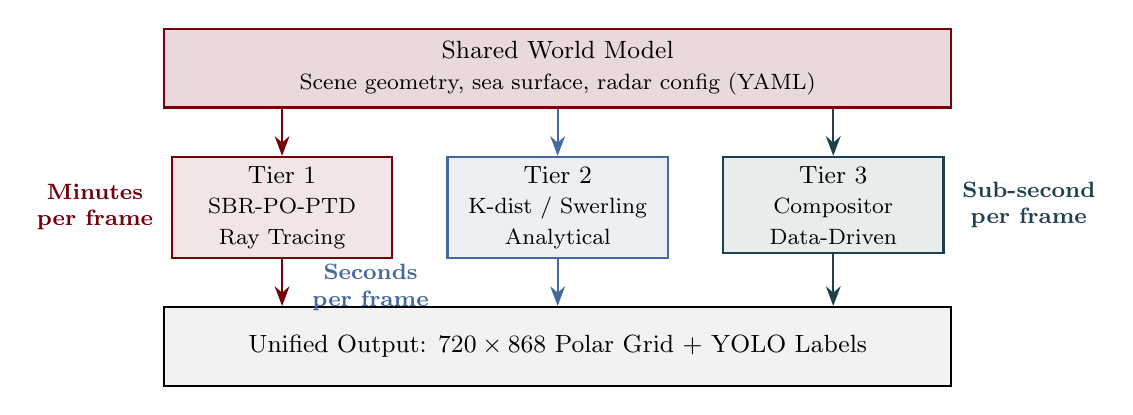
\begin{tikzpicture}[
    node distance=0.4cm and 1.0cm,
    block/.style={rectangle, draw, thick, minimum width=2.8cm, minimum height=1.0cm, align=center, font=\small},
    arrow/.style={-{Stealth[length=2.5mm]}, thick},
    label/.style={font=\footnotesize\bfseries, align=center}
]
% World Model (top)
\node[block, fill=Garnet!15, draw=Garnet, minimum width=10.0cm] (world) {Shared World Model\\{\footnotesize Scene geometry, sea surface, radar config (YAML)}};

% Three tiers
\node[block, fill=Garnet!10, draw=Garnet, below=0.6cm of world, xshift=-3.5cm] (t1) {Tier 1\\{\footnotesize SBR-PO-PTD}\\{\footnotesize Ray Tracing}};
\node[block, fill=CBlue!10, draw=CBlue, below=0.6cm of world] (t2) {Tier 2\\{\footnotesize K-dist / Swerling}\\{\footnotesize Analytical}};
\node[block, fill=CDark!10, draw=CDark, below=0.6cm of world, xshift=3.5cm] (t3) {Tier 3\\{\footnotesize Compositor}\\{\footnotesize Data-Driven}};

% Arrows from world model
\draw[arrow, Garnet] (world.south -| t1.north) -- (t1.north);
\draw[arrow, CBlue] (world.south) -- (t2.north);
\draw[arrow, CDark] (world.south -| t3.north) -- (t3.north);

% Output
\node[block, fill=black!5, draw=black, below=0.6cm of t2, minimum width=10.0cm] (output) {Unified Output: $720 \times 868$ Polar Grid + YOLO Labels};

\draw[arrow, Garnet] (t1.south) -- (t1.south |- output.north);
\draw[arrow, CBlue] (t2.south) -- (output.north);
\draw[arrow, CDark] (t3.south) -- (t3.south |- output.north);

% Annotations
\node[label, left=0.1cm of t1, Garnet] {Minutes\\per frame};
\node[label, below left=-0.05cm and 0.1cm of t2, CBlue] {Seconds\\per frame};
\node[label, right=0.1cm of t3, CDark] {Sub-second\\per frame};
\end{tikzpicture}
\caption{Three-tier simulation architecture. All tiers consume a shared YAML scene description and produce output on a common $720\times868$ polar grid with optional YOLO labels.}
\label{fig:architecture}
\end{figure}

Table~\ref{tab:tier_comparison} summarizes the key characteristics of each tier.

\begin{table}[htb]
\centering
\caption{Comparison of the three simulation tiers.}
\label{tab:tier_comparison}
\begin{tabular}{@{}lccc@{}}
\toprule
\textbf{Property} & \textbf{Tier 1} & \textbf{Tier 2} & \textbf{Tier 3} \\
\midrule
Fidelity & High & Medium & Low \\
Speed & Minutes/frame & Seconds/frame & Sub-second/frame \\
Physics & SBR-PO-PTD & Statistical & Data-driven \\
Sea clutter & FFT surface mesh & K-distribution & Real recordings \\
Targets & 3D mesh RCS & Swerling models & Extracted signatures \\
Multipath & Ray-level & Two-ray $F^4$ & Implicit \\
Output & Polar CSV + PNG & Polar CSV + PNG & Polar CSV + PNG \\
Use case & Validation & Training data & Domain transfer \\
\bottomrule
\end{tabular}
\end{table}

\subsection{World Model}
The shared world model defines a 3D scene composed of triangulated surface meshes for terrain and objects, positioned relative to the radar antenna location. The radar is placed at a configurable height above a reference datum and rotates through $360^\circ$ in discrete azimuth steps. The coordinate system is East-North-Up (ENU), with azimuth measured clockwise from north.

The sea surface is generated by spectral synthesis on a 2D spatial grid. In Tier~1 this surface is triangulated into a mesh for ray intersection; in Tier~2 it provides the statistical sea-state parameter that selects the K-distribution shape and scale; in Tier~3 the real sea clutter is already embedded in the recorded background frames.

Figure~\ref{fig:world_view} shows a 3D rendering of a representative world model, including the synthesized sea surface, terrain, and placed objects.

\begin{figure}[htb]
\centering
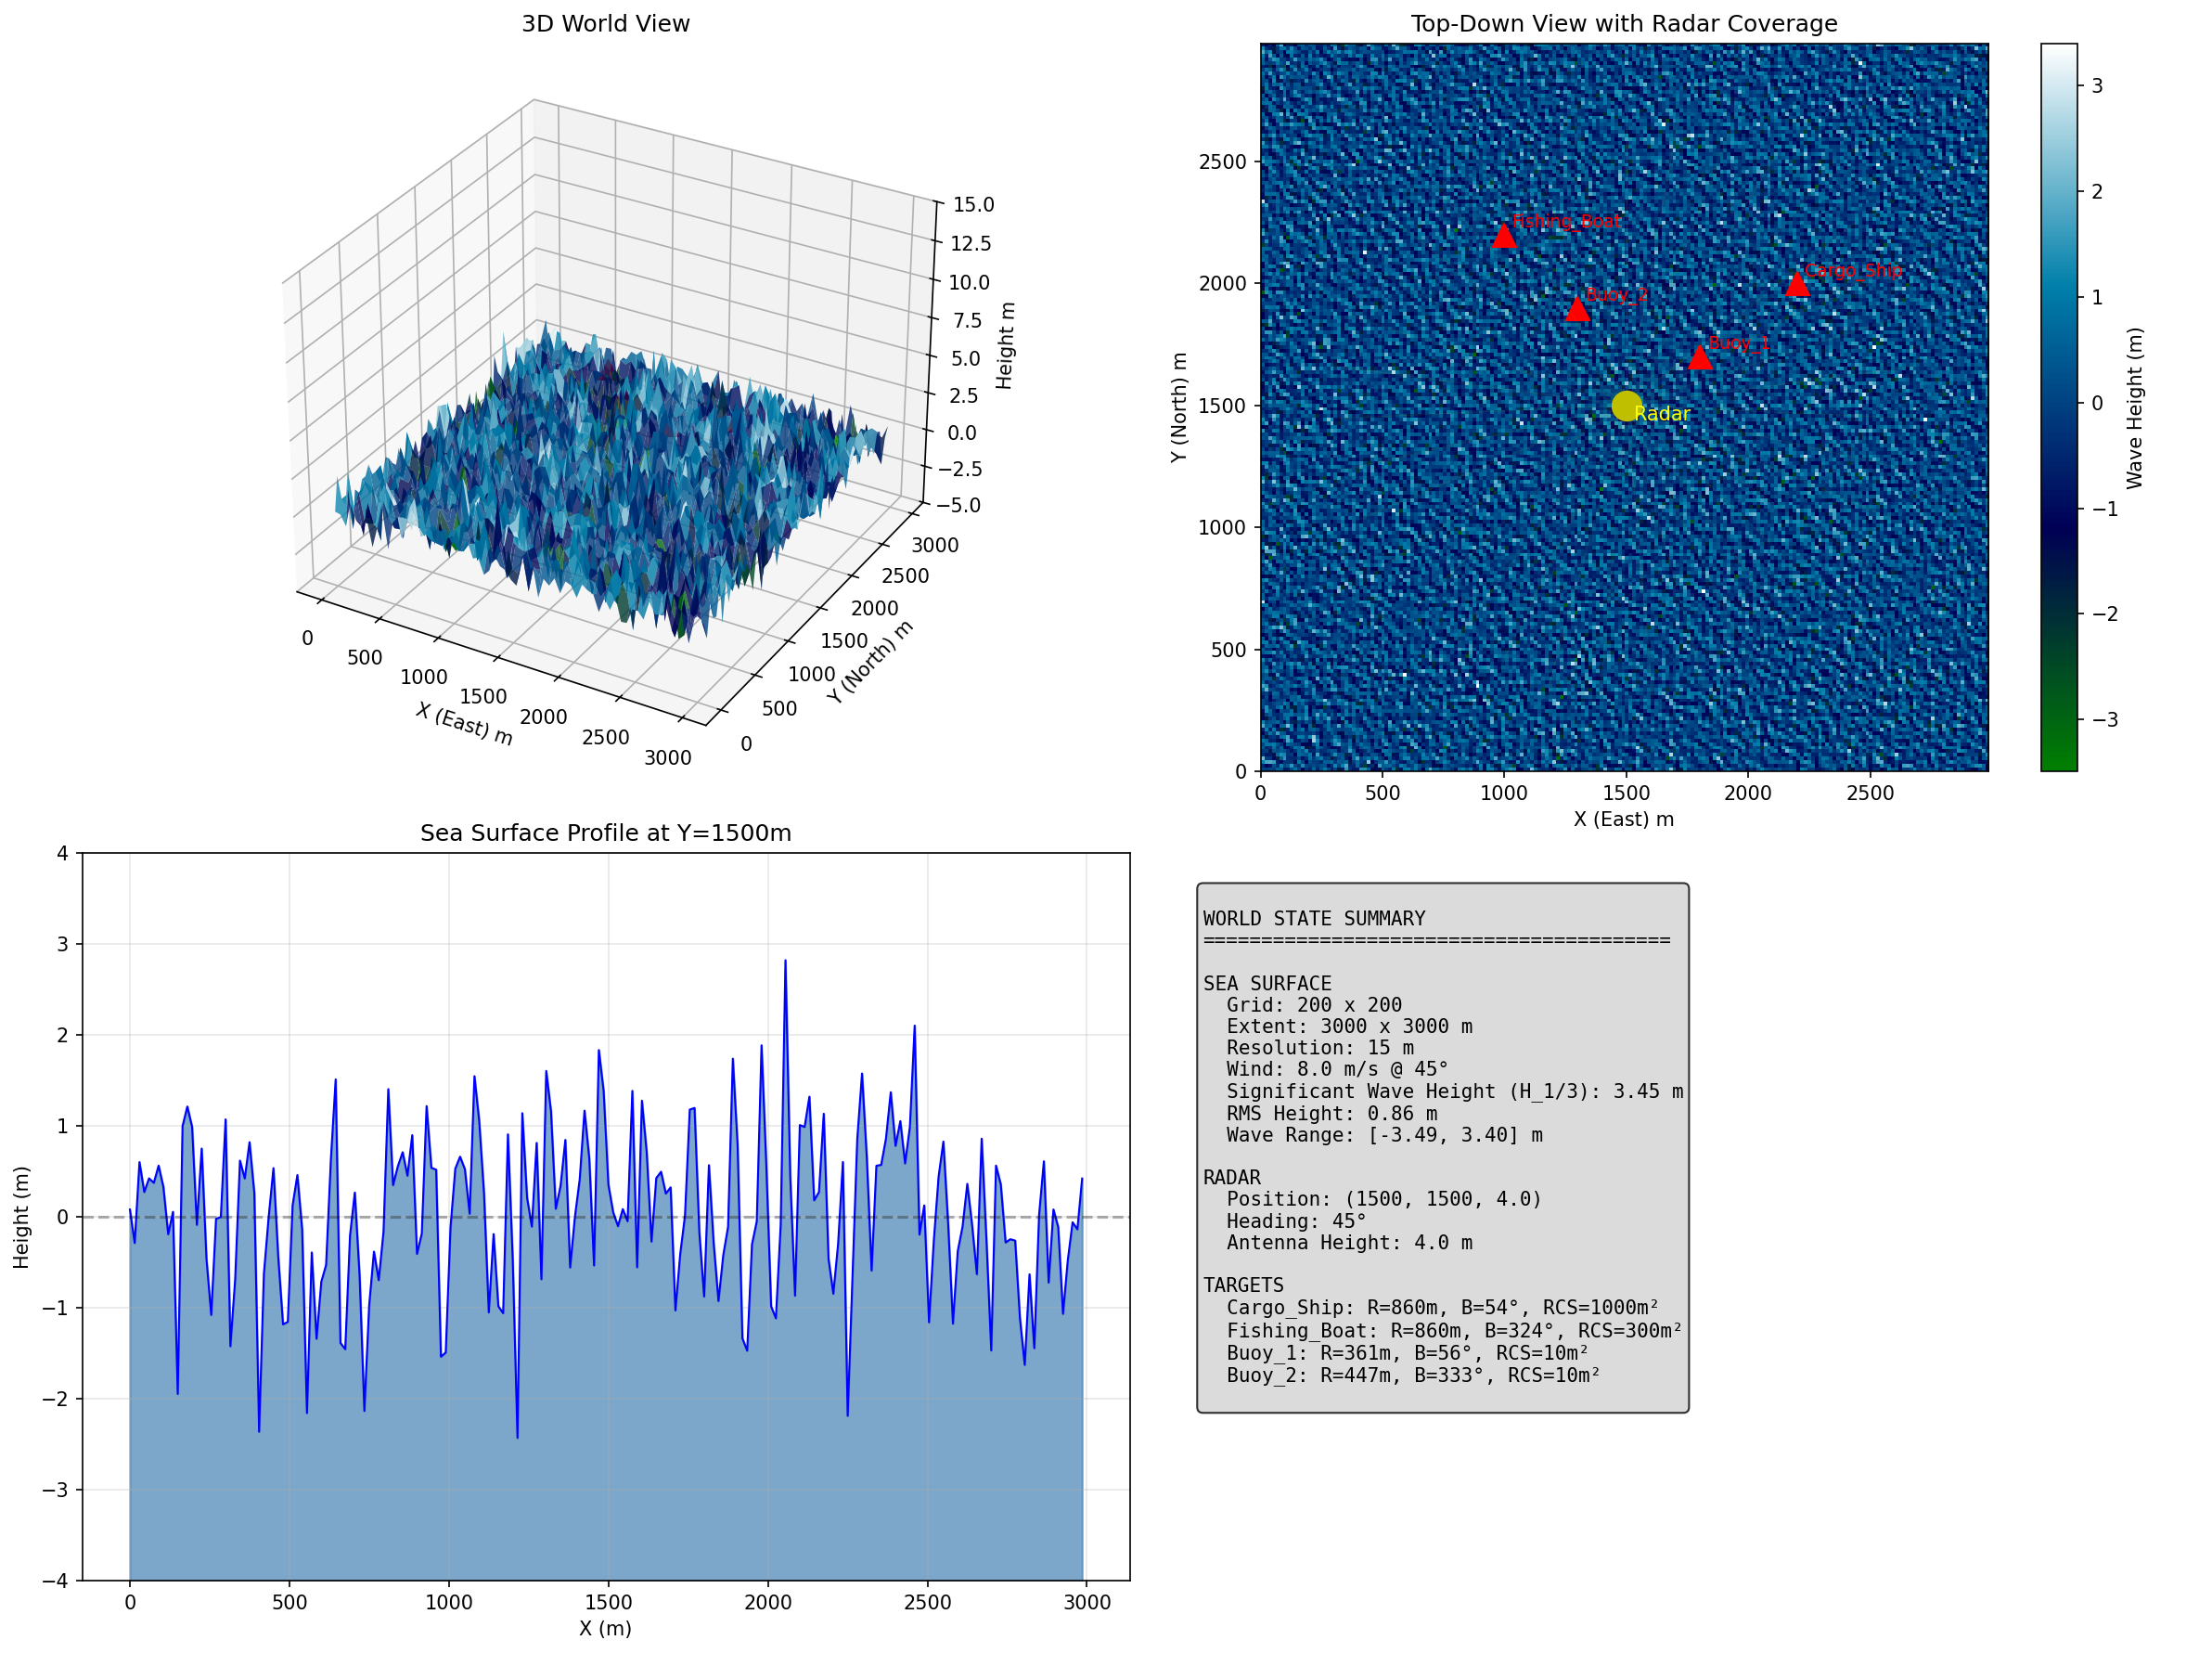
\includegraphics[width=0.85\columnwidth]{world_view_3d.png}
\caption{Three-dimensional world model visualization showing the synthesized sea surface, terrain, and scene objects.}
\label{fig:world_view}
\end{figure}

\subsection{Sea Surface Generation}
The sea surface elevation field $\eta(\mathbf{x}, t)$ is synthesized using the inverse FFT method of Tessendorf~\cite{Tessendorf2001}. The one-dimensional wave energy spectrum is specified as either the Pierson-Moskowitz (PM) spectrum~\cite{Pierson1964} for fully developed seas,
\begin{equation}\label{eq:pm}
S_{\mathrm{PM}}(\omega) = \frac{\alpha g^2}{\omega^5} \exp\!\left[-\beta\left(\frac{\omega_p}{\omega}\right)^{\!4}\right],
\end{equation}
where $\alpha = 8.1 \times 10^{-3}$, $\beta = 0.74$, and $\omega_p = g / U_{19.5}$ is the peak frequency determined by the wind speed $U_{19.5}$ at 19.5~m height, or the JONSWAP spectrum~\cite{Hasselmann1973} for fetch-limited conditions,
\begin{equation}\label{eq:jonswap}
S_{\mathrm{J}}(\omega) = S_{\mathrm{PM}}(\omega)\;\gamma^{\,\exp\!\left[-({\omega - \omega_p})^2 / (2\sigma^2\omega_p^2)\right]},
\end{equation}
with peak enhancement factor $\gamma = 3.3$ and spectral width $\sigma = 0.07$ ($\omega \leq \omega_p$) or $\sigma = 0.09$ ($\omega > \omega_p$). The deep-water linear dispersion relation $\omega^2 = gk$ maps frequency to wavenumber. Directional spreading is applied via a $\cos^{2s}$ distribution.

The 2D height field is obtained by assigning random phases to each spectral component and evaluating the inverse FFT:
\begin{equation}\label{eq:ifft_sea}
\eta(\mathbf{x}, t) = \sum_{\mathbf{k}} \hat{h}_0(\mathbf{k})\, e^{i(\mathbf{k}\cdot\mathbf{x} - \omega(\mathbf{k})\,t)} + \text{c.c.},
\end{equation}
where $\hat{h}_0(\mathbf{k})$ is drawn from $\mathcal{CN}(0, S(\mathbf{k})\,\Delta k_x\,\Delta k_y)$ and c.c.\ denotes the complex conjugate ensuring a real-valued surface. The default domain spans $2000 \times 2000$~m at 2~m resolution.

% ============================================================================
%  SECTION 4: TIER 1
% ============================================================================
\section{Tier 1: High-Fidelity Electromagnetic Ray Tracing}\label{sec:tier1}

Tier~1 provides the highest physical fidelity by tracing individual rays through the 3D scene geometry, computing scattered fields via PO and PTD at each interaction point, and constructing a synthetic radar return through coherent summation, pulse compression, and CFAR detection. The reference radar platform is the Furuno DRS4D-NXT solid-state marine radar, whose parameters are listed in Table~\ref{tab:radar_params}.

\begin{table}[htb]
\centering
\caption{Furuno DRS4D-NXT radar parameters used in Tier~1 simulation.}
\label{tab:radar_params}
\begin{tabular}{@{}lrl@{}}
\toprule
\textbf{Parameter} & \textbf{Value} & \textbf{Unit} \\
\midrule
Center frequency & 9.41 & GHz \\
Wavelength ($\lambda$) & 31.8 & mm \\
Bandwidth ($B$) & 50 & MHz \\
Transmit power ($P_t$) & 25 & W \\
Pulse width ($T$) & 10 & $\mu$s \\
Sample rate & 100 & MSPS \\
Antenna gain ($G$) & 22 & dBi \\
Horiz.\ beamwidth ($\theta_{\mathrm{3dB}}$) & 3.9 & deg \\
Vert.\ beamwidth & 25.0 & deg \\
Polarization & H & --- \\
Radome diameter & 0.61 & m \\
Range bins & 868 & --- \\
Azimuth samples & 720 & --- \\
Max range & 5556 & m \\
\bottomrule
\end{tabular}
\end{table}

\subsection{SBR-PO Architecture}
The Shooting and Bouncing Rays (SBR) method~\cite{Ling1989} launches a dense fan of rays from the radar antenna into the scene for each azimuth position. Each ray is intersected with the triangulated scene geometry using the M\"{o}ller-Trumbore algorithm~\cite{MollerTrumbore1997}. At each intersection, the Physical Optics (PO) contribution from the illuminated facet is computed, and the ray is specularly reflected for potential multi-bounce interactions. The framework supports four fidelity levels:
\begin{itemize}
    \item \textbf{Level 0}: Point-target radar equation (no geometry).
    \item \textbf{Level 1}: Line-of-sight blockage testing.
    \item \textbf{Level 2}: Single-bounce (two-ray) multipath.
    \item \textbf{Level 3}: Full multi-bounce SBR ray tracing.
\end{itemize}

Figure~\ref{fig:ray_tracing} illustrates the ray-tracing geometry for Level~3.

\begin{figure}[htb]
\centering
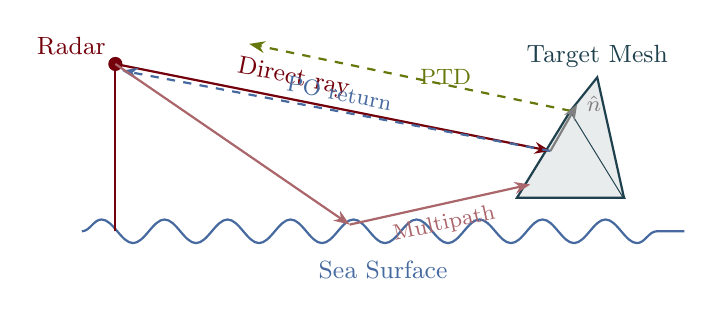
\begin{tikzpicture}[
    scale=0.85,
    arrow/.style={-{Stealth[length=2mm]}, thick},
    dasharrow/.style={-{Stealth[length=2mm]}, thick, dashed},
    every node/.style={font=\small}
]
% Sea surface
\draw[CBlue, thick, decorate, decoration={snake, amplitude=1.5mm, segment length=8mm}] (-0.5, 0) -- (8.5, 0);
\node[CBlue, below] at (4, -0.3) {Sea Surface};

% Radar
\fill[Garnet] (0, 2.5) circle (3pt);
\node[Garnet, above left] at (0, 2.5) {Radar};
\draw[Garnet, thick] (0, 0) -- (0, 2.5);

% Target mesh
\draw[CDark, thick, fill=CDark!10] (6, 0.5) -- (6.8, 1.8) -- (7.6, 0.5) -- cycle;
\draw[CDark, thick, fill=CDark!10] (6.8, 1.8) -- (7.2, 2.3) -- (7.6, 0.5);
\node[CDark, above] at (7.2, 2.3) {Target Mesh};

% Direct ray
\draw[arrow, Garnet] (0, 2.5) -- node[above, sloped, pos=0.4] {Direct ray} (6.5, 1.2);

% PO scatter
\draw[dasharrow, CBlue] (6.5, 1.2) -- node[above, sloped, pos=0.5] {\footnotesize PO return} (0.1, 2.4);

% Surface bounce ray
\draw[arrow, Garnet!60] (0, 2.5) -- (3.5, 0.1);
\draw[arrow, Garnet!60] (3.5, 0.1) -- node[below, sloped, pos=0.5] {\footnotesize Multipath} (6.2, 0.7);

% PTD edge
\draw[dasharrow, COlive] (6.8, 1.8) -- node[right, pos=0.5] {\footnotesize PTD} (2, 2.8);

% Facet normal
\draw[arrow, black!50] (6.5, 1.2) -- ++(0.4, 0.7);
\node[black!50, right, font=\footnotesize] at (6.9, 1.9) {$\hat{n}$};
\end{tikzpicture}
\caption{Tier~1 ray-tracing geometry. Rays launched from the radar intersect scene meshes; PO computes the scattered field from illuminated facets, and PTD adds edge diffraction contributions. Surface-reflected rays model multipath.}
\label{fig:ray_tracing}
\end{figure}

\subsection{Physical Optics Scattering}
For each illuminated triangular facet with area $A_i$ and outward unit normal $\hat{n}_i$, the PO monostatic scattered field is computed using the Gordon integral approximation~\cite{Gordon1975}:
\begin{equation}\label{eq:po}
E_s = \sum_{i \in \mathcal{I}} \cos\theta_i \; A_i \; e^{\,j2k\,r_i},
\end{equation}
where $\mathcal{I}$ is the set of illuminated facets satisfying $\cos\theta_i = -\hat{n}_i \cdot \hat{k}_{\mathrm{inc}} > 0$, $k = 2\pi/\lambda$ is the wavenumber, $r_i$ is the distance from the radar to the facet centroid, and the factor of 2 in the exponent accounts for two-way propagation. The monostatic RCS is then
\begin{equation}\label{eq:rcs_po}
\sigma_{\mathrm{PO}} = \frac{4\pi}{\lambda^2}\left|\sum_{i \in \mathcal{I}} \cos\theta_i \; A_i \; e^{\,j2k\,r_i}\right|^2.
\end{equation}

\subsection{PTD Edge Diffraction}
Physical Optics produces accurate results for electrically large, smooth surfaces but underestimates scattering from edges and discontinuities. The Physical Theory of Diffraction~\cite{Ufimtsev2007} adds a non-uniform edge current correction. For each mesh edge of length $\ell_e$, PTD computes a diffraction coefficient $D_e$ based on the edge geometry and incidence angle. The total scattered field combines PO and PTD contributions coherently:
\begin{equation}\label{eq:total_field}
E_{\mathrm{total}} = E_{\mathrm{PO}} + E_{\mathrm{PTD}}.
\end{equation}

\subsection{Coherent Summation and Radar Equation}
For a given azimuth pointing direction, all scattering contributions along each range bin are summed coherently to form the received voltage:
\begin{equation}\label{eq:vrx}
V_{\mathrm{rx}}(R) = \sum_{i} \frac{A_i\,\sqrt{\sigma_i}}{R_i^2}\, e^{-j2kR_i},
\end{equation}
where the amplitude factor incorporates the radar equation~\cite{Skolnik2008}:
\begin{equation}\label{eq:radar_eq}
P_r = \frac{P_t\, G^2\, \lambda^2\, \sigma}{(4\pi)^3\, R^4\, L},
\end{equation}
with system loss $L$ aggregating atmospheric attenuation and component losses.

\subsection{LFM Pulse Compression}
The transmit waveform is a linear frequency modulation (LFM) chirp~\cite{Cook1967} with time-bandwidth product $BT = 50 \times 10^6 \times 10 \times 10^{-6} = 500$:
\begin{equation}\label{eq:lfm}
s(t) = \exp\!\left(j\pi K t^2\right), \quad 0 \leq t \leq T,
\end{equation}
where $K = B/T = 5 \times 10^{12}$~Hz/s is the chirp rate. Pulse compression is performed via frequency-domain matched filtering:
\begin{equation}\label{eq:matched_filter}
y(t) = \mathcal{F}^{-1}\!\left[\mathcal{F}\{r(t)\} \cdot \mathcal{F}^*\{s(t)\}\right],
\end{equation}
where $r(t)$ is the received signal. A Taylor window is applied to suppress range sidelobes from the theoretical $-13.3$~dB (unwindowed sinc) to approximately $-35$~dB at the cost of modest mainlobe broadening. Figure~\ref{fig:pulse_compression} shows the pulse compression output with Taylor windowing.

\begin{figure}[htb]
\centering
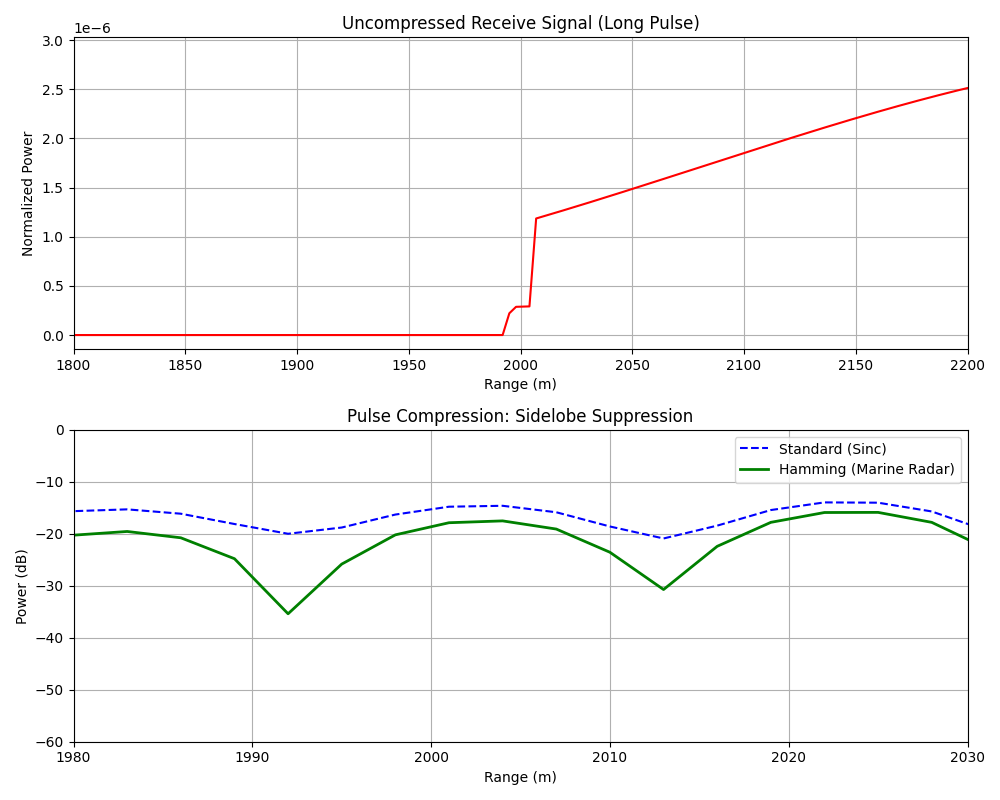
\includegraphics[width=0.9\columnwidth]{pulse_compression_windowed.png}
\caption{Pulse compression output with Taylor windowing. The matched filter concentrates the chirp energy into a narrow range cell, achieving approximately $\SI{27}{dB}$ compression gain.}
\label{fig:pulse_compression}
\end{figure}

\subsection{CFAR Detection}
Target detection is performed using a Cell-Averaging Constant False Alarm Rate (CA-CFAR) processor~\cite{Rohling1983}. For each cell under test (CUT), the noise power is estimated from $N = 32$ training cells (16 on each side), separated from the CUT by 4 guard cells on each side. The adaptive threshold is
\begin{equation}\label{eq:cfar}
T_{\mathrm{CFAR}} = \alpha \cdot \hat{\sigma}_n^2, \quad \alpha = N\left(P_{\mathrm{fa}}^{-1/N} - 1\right),
\end{equation}
where $P_{\mathrm{fa}} = 10^{-6}$ is the design false-alarm probability. For $N = 32$, this yields a threshold multiplier $\alpha \approx 22.9$. An ordered-statistic CFAR (OS-CFAR) variant~\cite{Gandhi1988} is also available for improved performance at clutter boundaries.

\subsection{Validation: Corner Reflector RCS}
Figure~\ref{fig:corner_reflector} compares the simulated RCS of a 3-inch (76.2~mm) trihedral corner reflector against the analytical prediction $\sigma = 12\pi a^4/\lambda^2$. At 9.41~GHz ($\lambda = 31.8$~mm), the analytical RCS is $\sigma = 0.082$~m$^2$, and the PO-computed value agrees within the expected margin for this electrically moderate target ($a/\lambda \approx 2.4$).

\begin{figure}[htb]
\centering
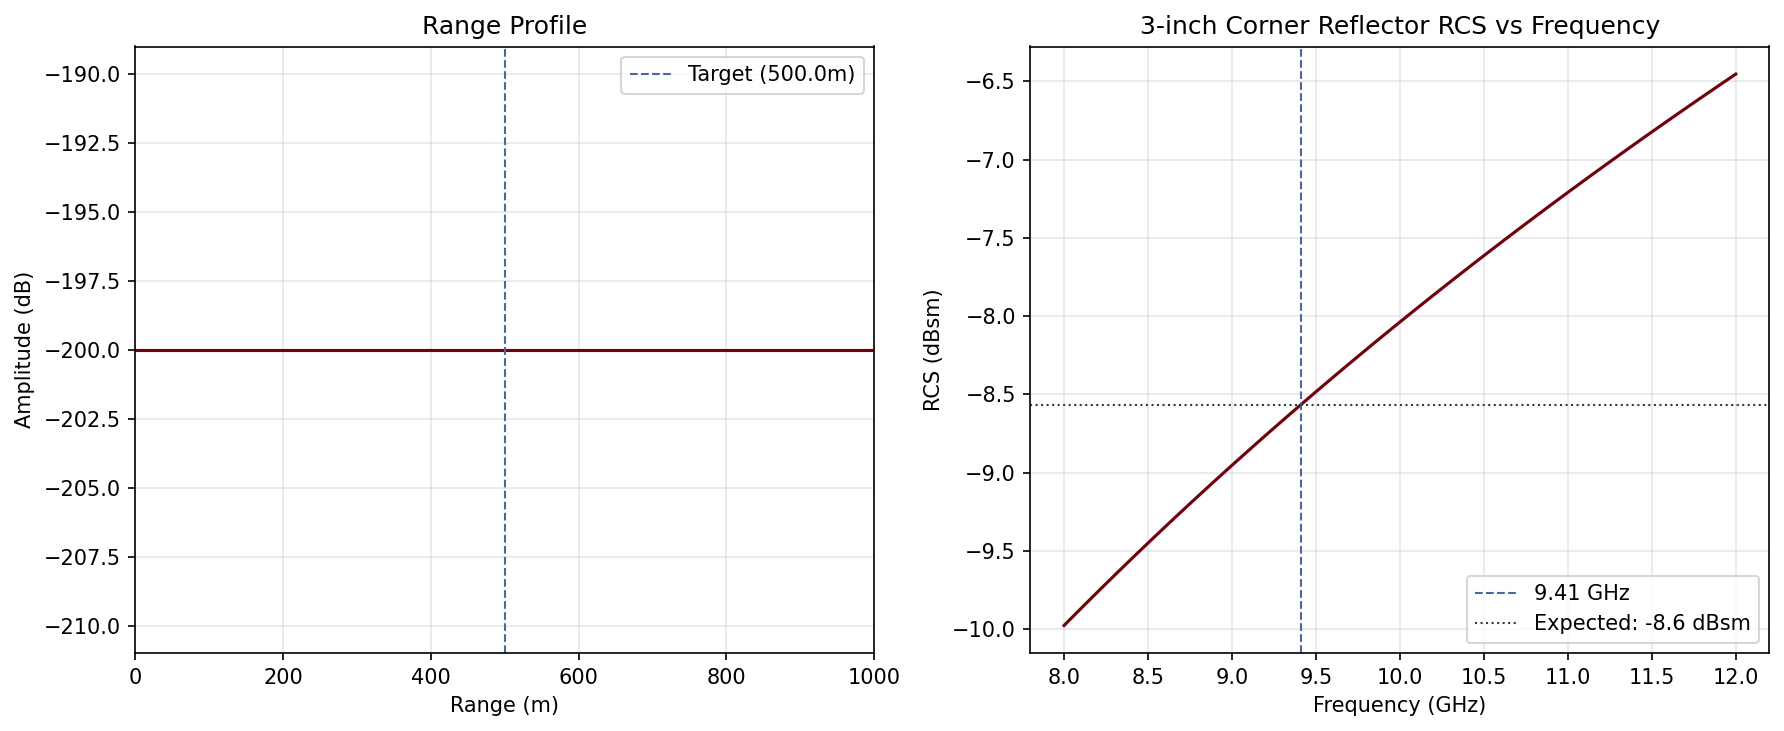
\includegraphics[width=0.9\columnwidth]{corner_reflector_validation.png}
\caption{Corner reflector RCS validation. Simulated PO return from a 3-inch trihedral reflector compared with the analytical cross section at 9.41~GHz.}
\label{fig:corner_reflector}
\end{figure}

Figure~\ref{fig:ray_slice} shows a ray-slice visualization demonstrating ray propagation through a representative scene geometry, illustrating both direct and surface-reflected paths.

\begin{figure}[htb]
\centering
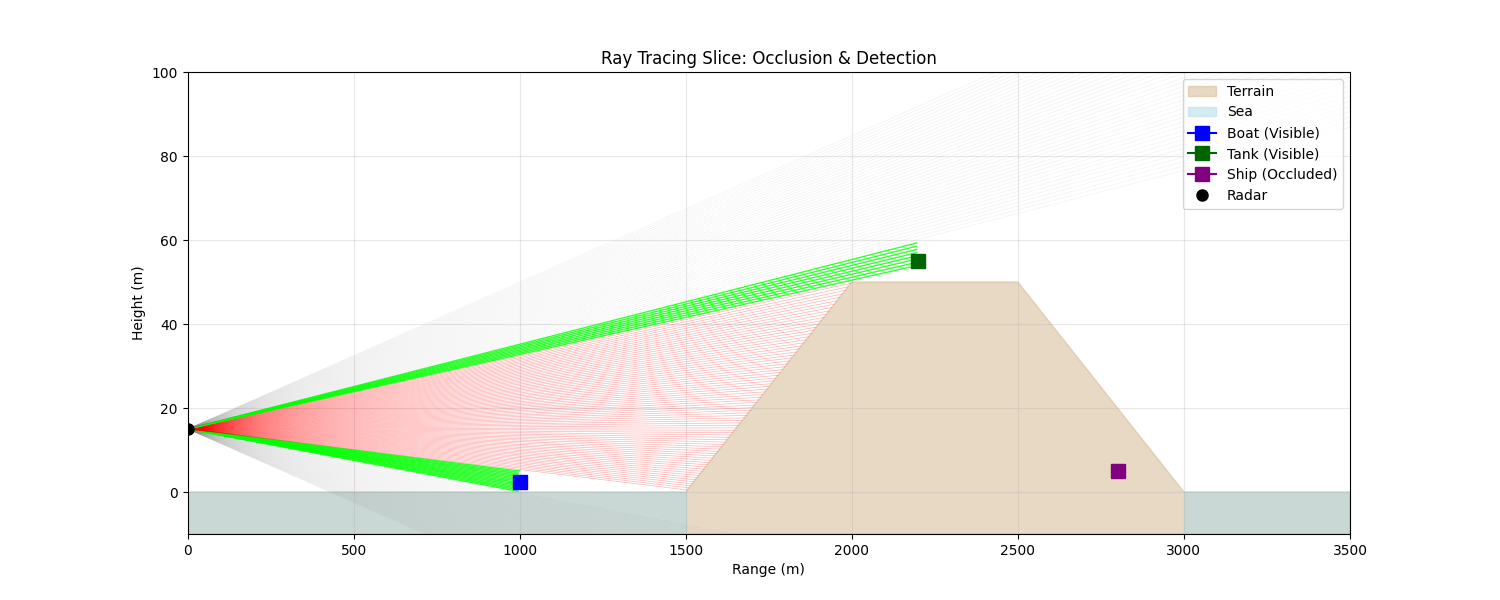
\includegraphics[width=0.9\columnwidth]{ray_slice_demo.png}
\caption{Ray-slice visualization showing direct and multipath ray propagation through scene geometry in the elevation plane.}
\label{fig:ray_slice}
\end{figure}

% ============================================================================
%  SECTION 5: TIER 2
% ============================================================================
\section{Tier 2: Analytical Approximation}\label{sec:tier2}

Tier~2 replaces the explicit ray-tracing computation with closed-form statistical models, reducing per-frame generation time from minutes to seconds while preserving the essential radar phenomenology.

\subsection{K-Distribution Sea Clutter}
Sea clutter at X-band and low grazing angles is modeled as a compound process~\cite{Ward1981, Ward2013}: a slowly varying texture component drawn from a gamma distribution modulates an exponential speckle process. The resulting K-distribution probability density function (PDF) is
\begin{equation}\label{eq:kdist}
p(x) = \frac{2}{\Gamma(\nu)} \left(\frac{\nu x}{\mu}\right)^{\!\nu/2} K_{\nu-1}\!\left(2\sqrt{\frac{\nu x}{\mu}}\right),
\end{equation}
where $\nu$ is the shape parameter controlling the tail heaviness (smaller $\nu$ produces heavier tails corresponding to spikier clutter), $\mu$ is the scale parameter representing the mean clutter power, and $K_{\nu-1}(\cdot)$ is the modified Bessel function of the second kind. Table~\ref{tab:sea_state} lists the shape and scale parameters for Douglas sea states 0--7.

\begin{table}[htb]
\centering
\caption{K-distribution parameters by Douglas sea state.}
\label{tab:sea_state}
\begin{tabular}{@{}clcc@{}}
\toprule
\textbf{State} & \textbf{Description} & \textbf{Shape $\nu$} & \textbf{Scale $\mu$ (W)} \\
\midrule
0 & Glassy calm   & 50.0 & $1\times10^{-12}$ \\
1 & Calm          & 20.0 & $5\times10^{-12}$ \\
2 & Smooth        & 10.0 & $2\times10^{-11}$ \\
3 & Slight        &  5.0 & $1\times10^{-10}$ \\
4 & Moderate      &  2.0 & $5\times10^{-10}$ \\
5 & Rough         &  1.0 & $2\times10^{-9}$ \\
6 & Very rough    &  0.5 & $1\times10^{-8}$ \\
7 & High          &  0.2 & $5\times10^{-8}$ \\
\bottomrule
\end{tabular}
\end{table}

Spatial correlation is imposed by convolving the independent clutter samples with an exponential kernel $k(\Delta r) = \exp(-|\Delta r|/r_c)$ in the range direction, where $r_c$ is the correlation length. Grazing-angle dependence is modeled empirically as $\mu(\psi) = \mu_0 (\sin 5^\circ / \sin\psi)^{1.5}$, normalized to a reference grazing angle of $5^\circ$.

\subsection{Swerling Target Models}
Target RCS fluctuations are modeled using the five Swerling cases~\cite{Swerling1960}. Case~0 is non-fluctuating (deterministic $\sigma$). Cases~1 and~2 model targets with many comparable scatterers, producing an exponential RCS distribution:
\begin{equation}\label{eq:sw12}
p(\sigma) = \frac{1}{\sigma_m} \exp\!\left(-\frac{\sigma}{\sigma_m}\right), \quad \sigma \geq 0,
\end{equation}
where $\sigma_m$ is the mean RCS. Cases~3 and~4 model targets with one dominant scatterer plus many smaller ones, yielding a chi-squared distribution with four degrees of freedom:
\begin{equation}\label{eq:sw34}
p(\sigma) = \frac{4\sigma}{\sigma_m^2} \exp\!\left(-\frac{2\sigma}{\sigma_m}\right), \quad \sigma \geq 0.
\end{equation}
The odd cases (1, 3) fluctuate scan-to-scan (correlated within a single scan), while the even cases (2, 4) fluctuate pulse-to-pulse.

\subsection{Two-Ray Multipath Propagation}
Over-water propagation at low grazing angles produces a strong surface-reflected multipath component that interferes constructively and destructively with the direct path~\cite{Blake1980}. The one-way propagation factor is
\begin{equation}\label{eq:multipath}
F = \left|1 + \rho\,\rho_s\, e^{-jk\Delta R}\right|,
\end{equation}
where $\rho$ is the Fresnel reflection coefficient for horizontal polarization over seawater ($\varepsilon_r \approx 80 + 70j$, $\sigma_c = 4$~S/m),
\begin{equation}\label{eq:fresnel}
\rho_H = \frac{\sin\psi - \sqrt{\varepsilon_r - \cos^2\psi}}{\sin\psi + \sqrt{\varepsilon_r - \cos^2\psi}},
\end{equation}
$\rho_s$ is the Ament roughness reduction factor~\cite{Ament1953} accounting for surface wave height, and the path difference for the flat-earth approximation is $\Delta R = 2h_1 h_2 / R$. The two-way radar equation includes the propagation factor as $F^4$:
\begin{equation}\label{eq:radar_multipath}
P_r = \frac{P_t\, G^2\, \lambda^2\, \sigma\, F^4}{(4\pi)^3\, R^4\, L}.
\end{equation}

\subsection{Output Quantization}
The continuous-valued radar return is quantized to 4-bit (16 levels) or 8-bit (256 levels) to match the Furuno DRS4D-NXT digital output format, with logarithmic scaling applied prior to quantization.

\subsection{Tier 2 Output Examples}
Figure~\ref{fig:tier2_output} shows representative Tier~2 outputs for three scenarios: a mixed land-and-water scene, an open-water scene with maritime targets, and a high sea-state clutter environment.

\begin{figure}[htb]
\centering
\begin{subcaptionblock}{0.32\columnwidth}
    \centering
    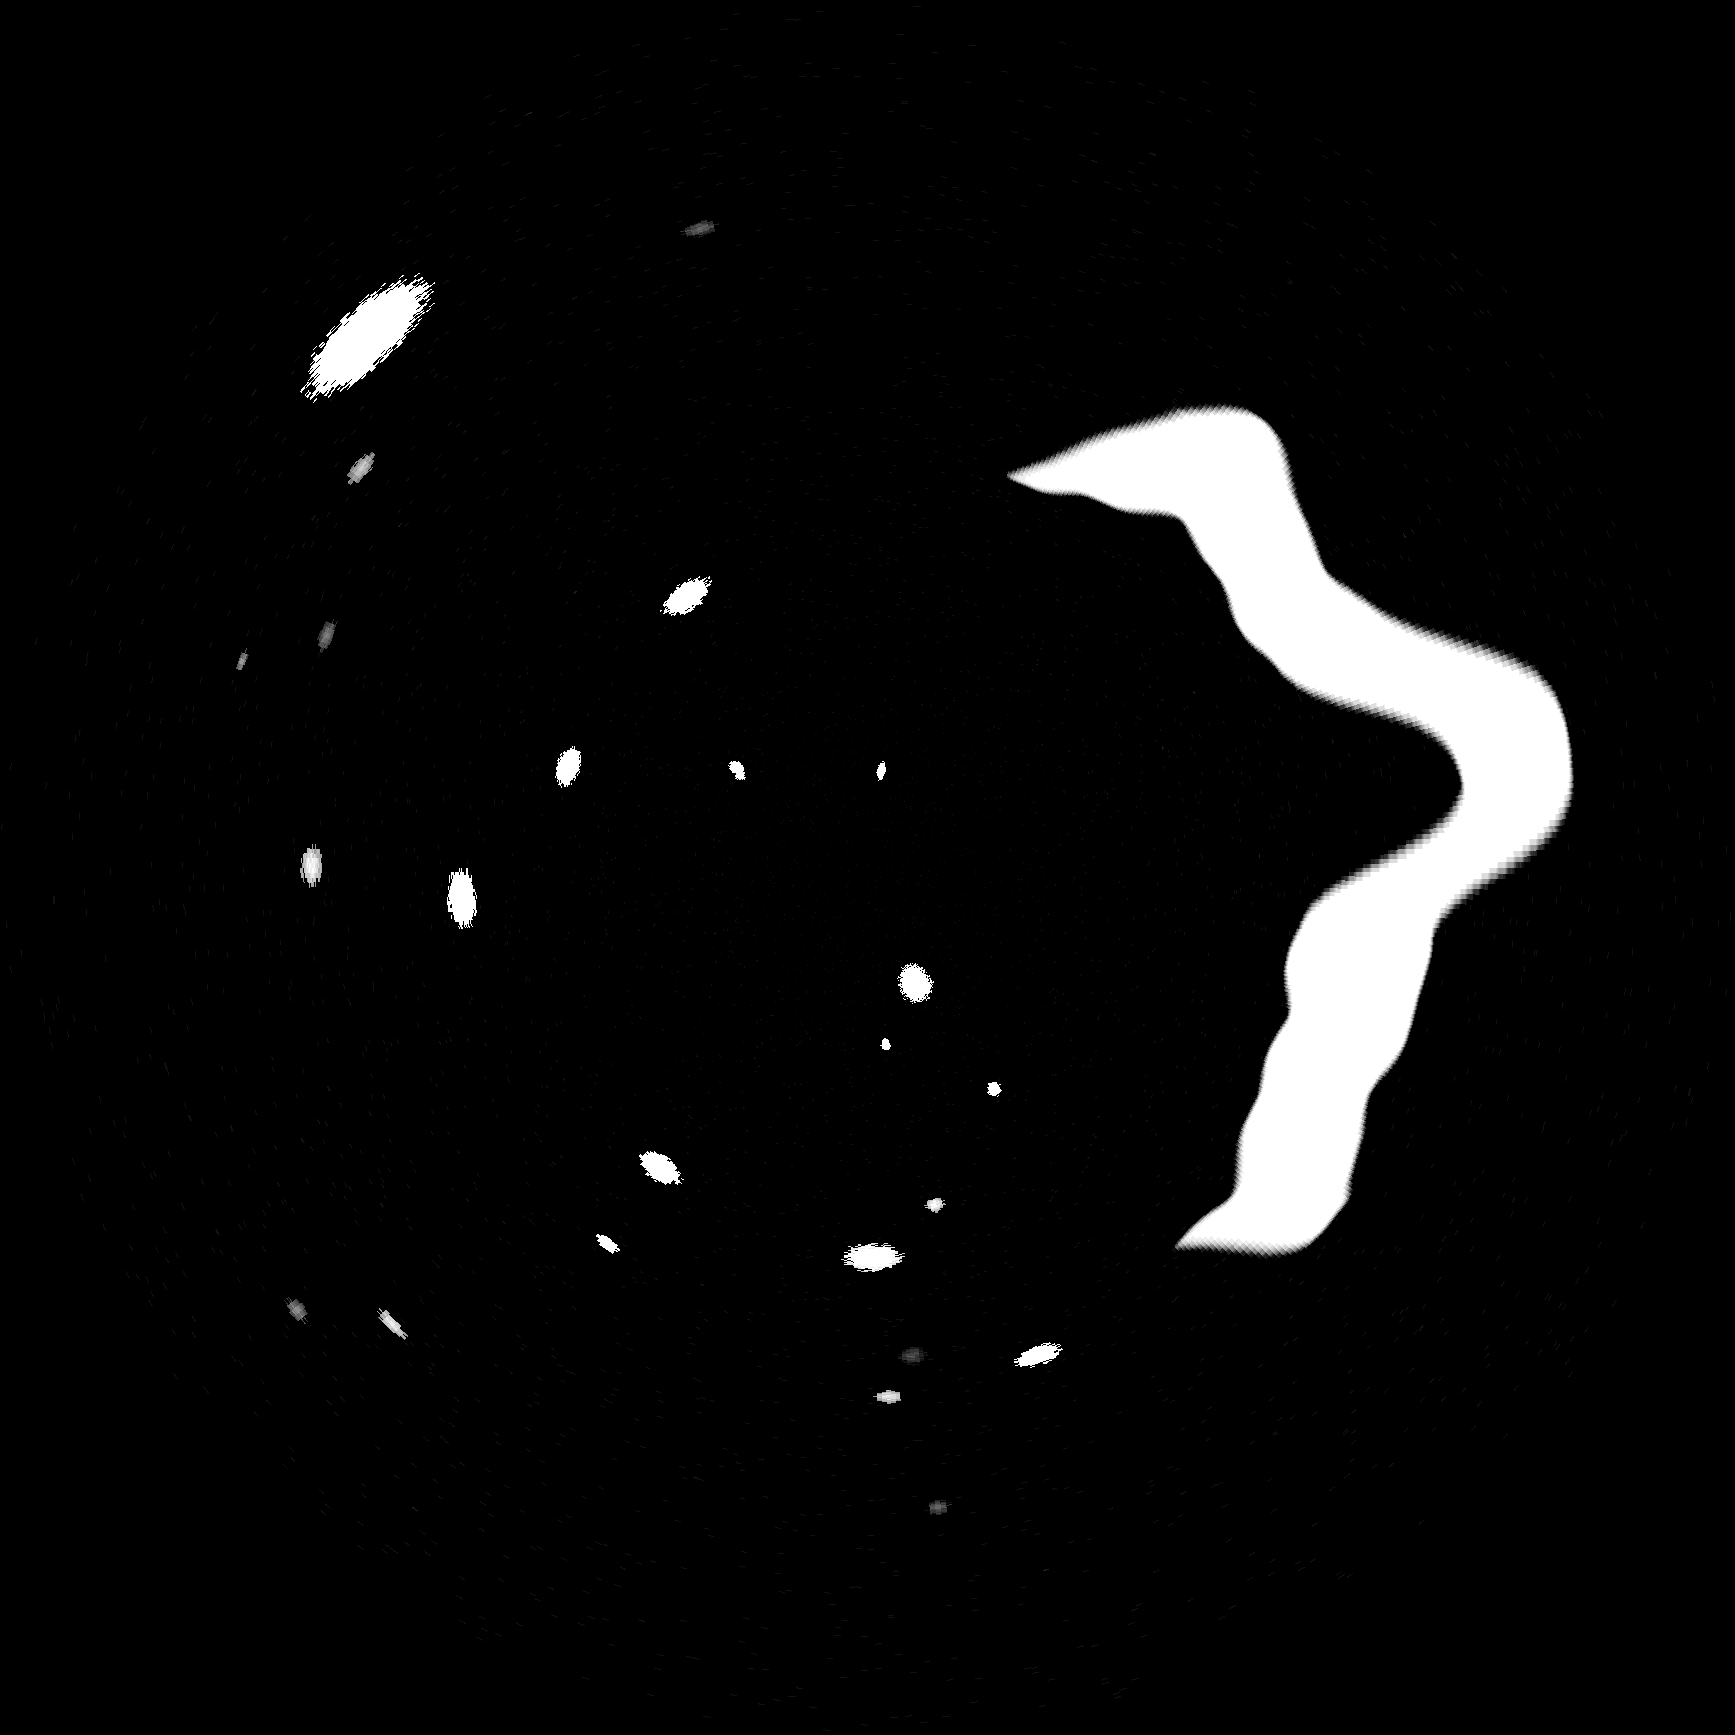
\includegraphics[width=\linewidth]{land_and_targets.png}
    \caption{Land + targets}
\end{subcaptionblock}
\hfill
\begin{subcaptionblock}{0.32\columnwidth}
    \centering
    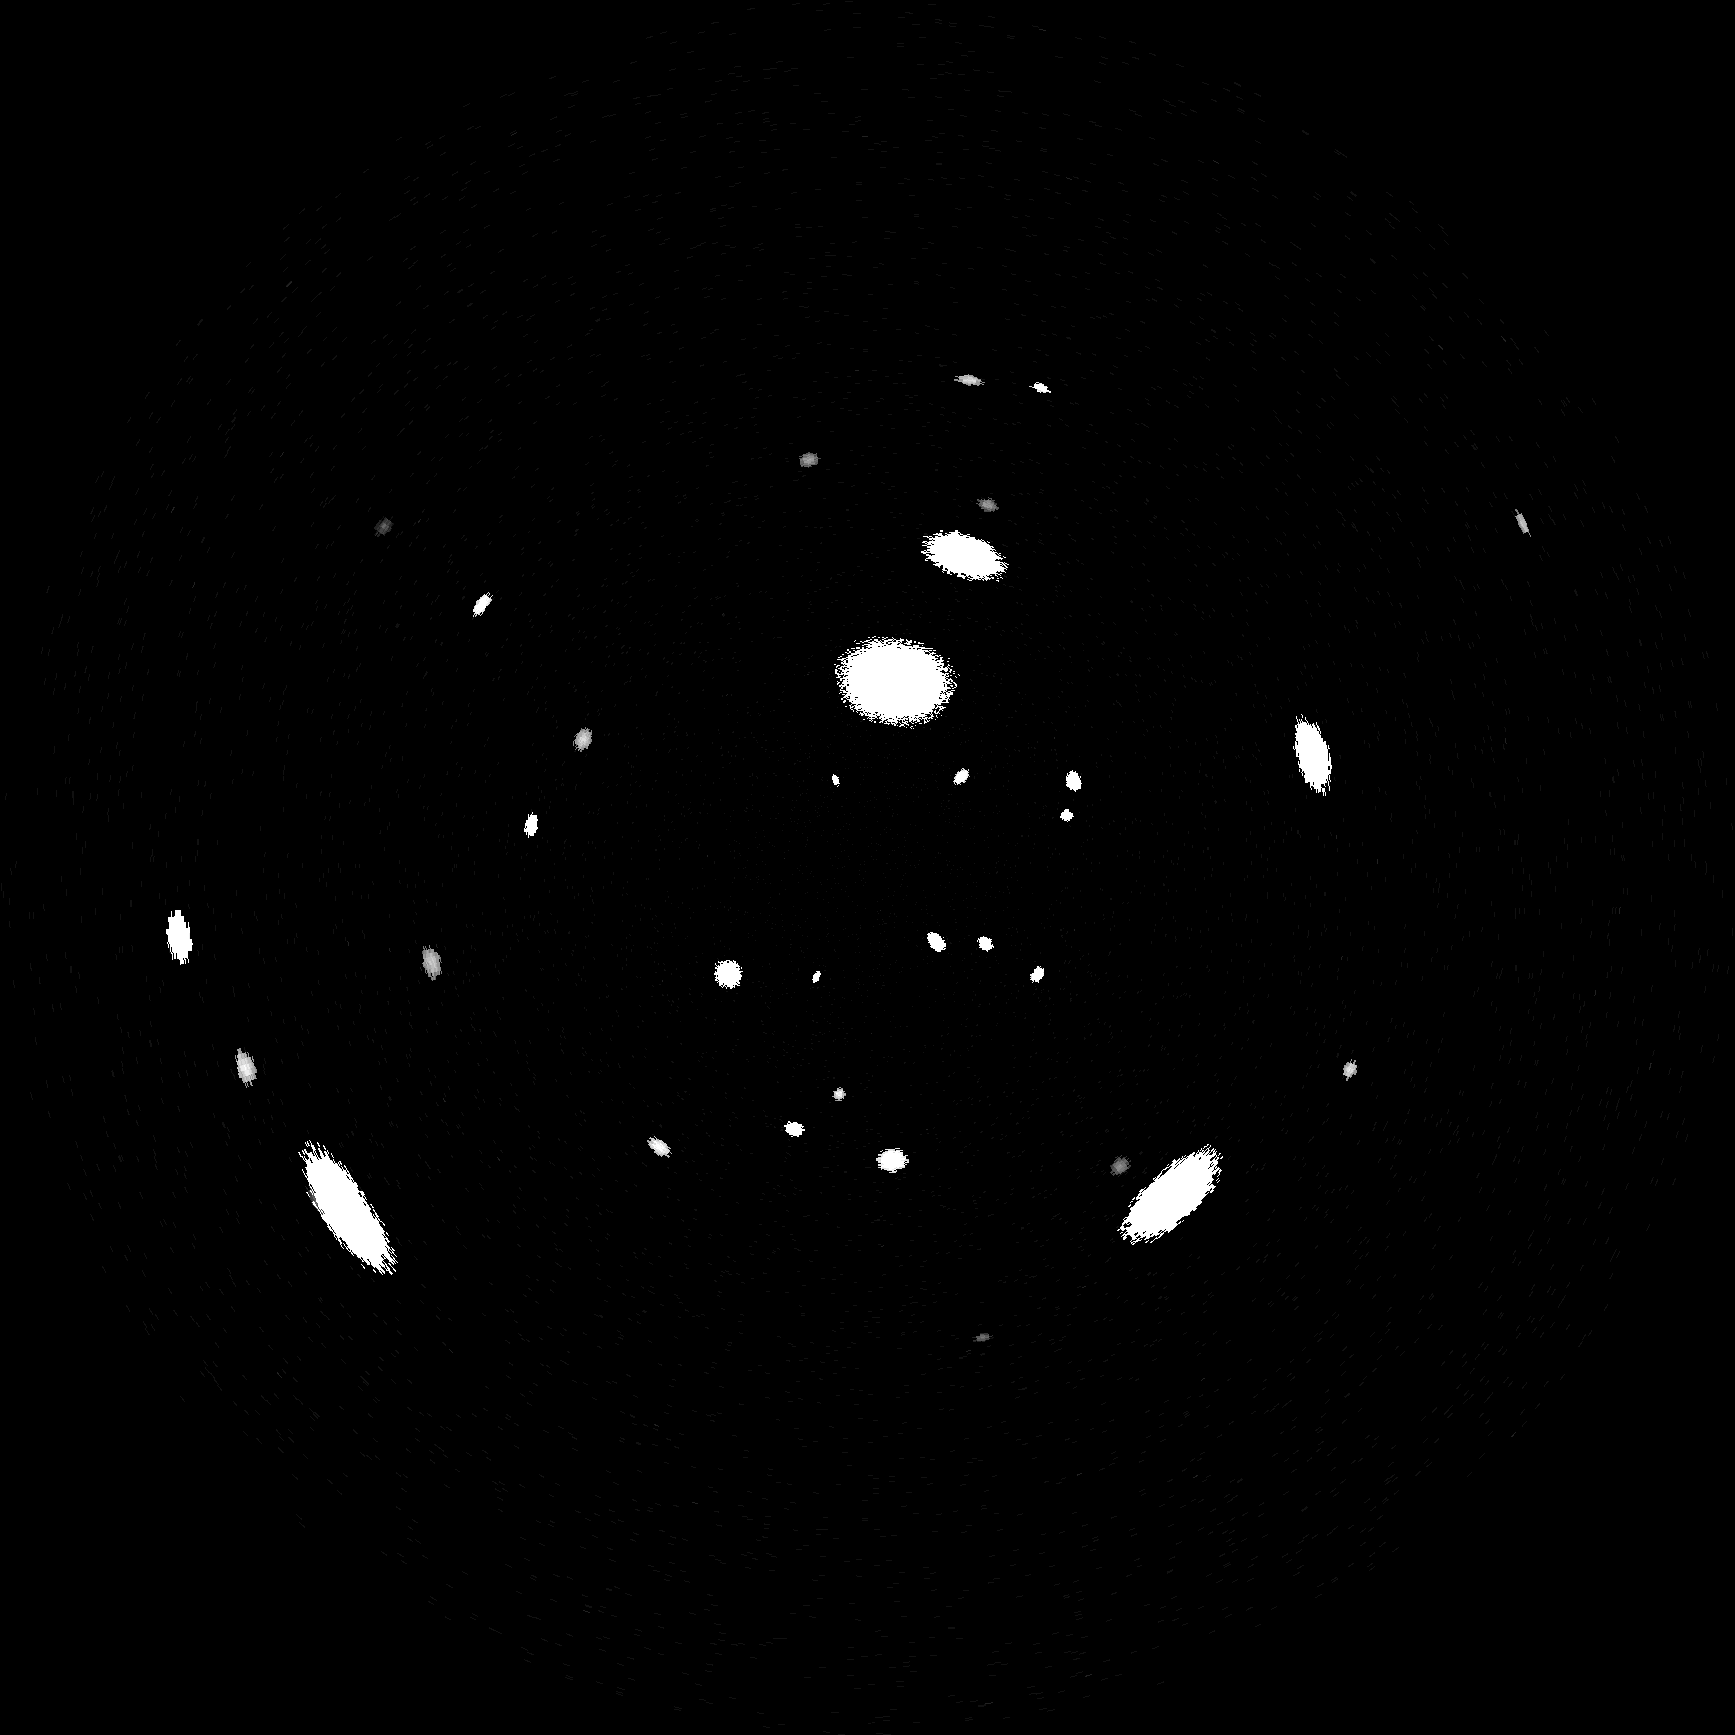
\includegraphics[width=\linewidth]{water_targets.png}
    \caption{Water targets}
\end{subcaptionblock}
\hfill
\begin{subcaptionblock}{0.32\columnwidth}
    \centering
    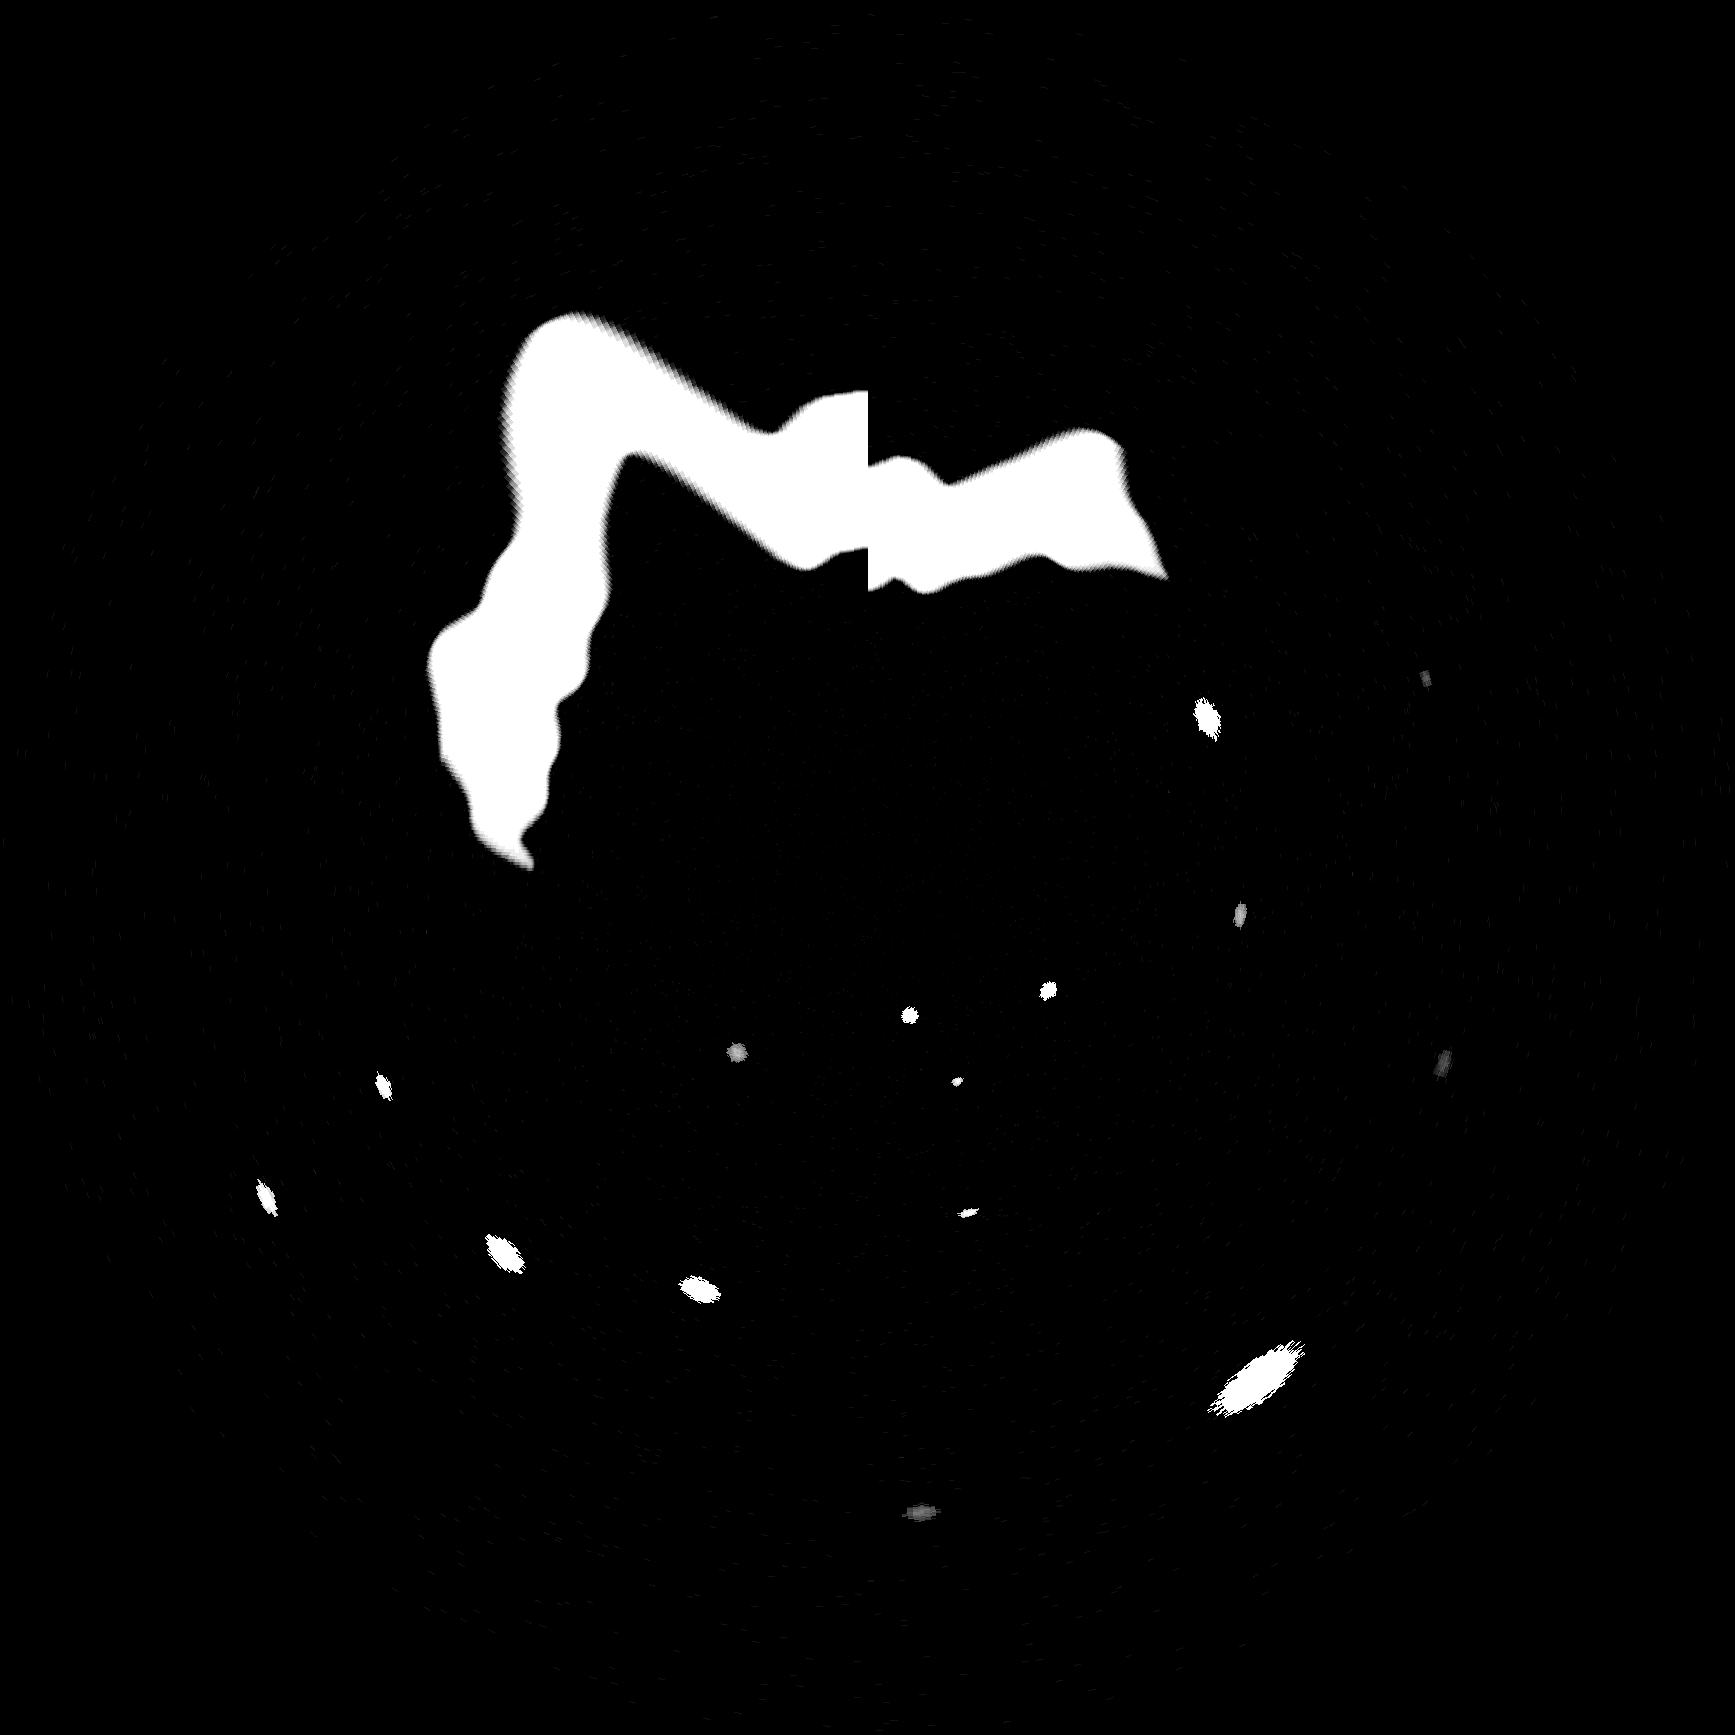
\includegraphics[width=\linewidth]{high_sea_state.png}
    \caption{High sea state}
\end{subcaptionblock}
\caption{Tier~2 analytical outputs. (a)~Mixed land and maritime target scene. (b)~Open-water scene with vessel and buoy targets. (c)~High sea-state clutter (state~6--7) demonstrating spiky K-distribution returns.}
\label{fig:tier2_output}
\end{figure}

% ============================================================================
%  SECTION 6: TIER 3
% ============================================================================
\section{Tier 3: Data-Driven Compositor}\label{sec:tier3}

Tier~3 bridges the simulation-to-reality gap by operating directly on recorded Furuno DRS4D-NXT radar data. Rather than generating synthetic radar returns from physical models, it extracts real object signatures from annotated recordings and composites them into existing background frames with configurable motion, intensity modulation, and YOLO-compatible labeling. This approach preserves the authentic noise characteristics, clutter texture, and sensor artifacts of the physical radar.

\subsection{Rust-Based Extraction Pipeline}
Object signatures are extracted from recorded radar data using a set of tools implemented in Rust for performance. The pipeline comprises three components:
\begin{itemize}
    \item \textbf{Radar Annotator}: A graphical tool for manually labeling objects of interest in recorded polar-coordinate CSV frames, producing bounding-box annotations with class identifiers.
    \item \textbf{Scene Extractor}: Segments annotated regions from each frame, storing the intensity data and binary mask for later compositing.
    \item \textbf{Land Extractor}: Identifies water/land boundaries from accumulated radar returns, producing a binary water mask that constrains object placement during synthesis.
\end{itemize}

\subsection{Six-Stage Synthesis Pipeline}
The Python compositor implements a six-stage pipeline, illustrated in Figure~\ref{fig:compositor_pipeline}:

\begin{figure}[htb]
\centering
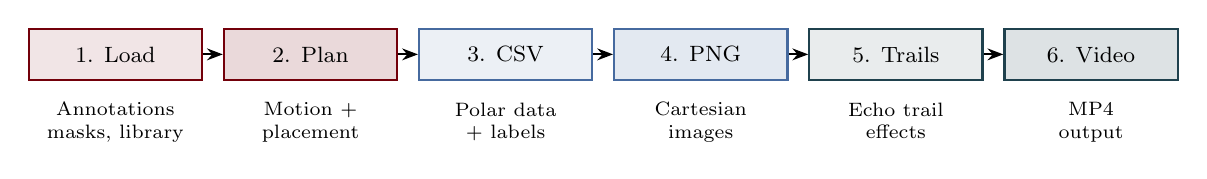
\begin{tikzpicture}[
    node distance=0.25cm,
    stage/.style={rectangle, draw, thick, minimum width=2.2cm, minimum height=0.65cm, align=center, font=\footnotesize},
    arrow/.style={-{Stealth[length=2mm]}, thick}
]
\node[stage, fill=Garnet!10, draw=Garnet] (s1) {1. Load};
\node[stage, fill=Garnet!15, draw=Garnet, right=of s1] (s2) {2. Plan};
\node[stage, fill=CBlue!10, draw=CBlue, right=of s2] (s3) {3. CSV};
\node[stage, fill=CBlue!15, draw=CBlue, right=of s3] (s4) {4. PNG};
\node[stage, fill=CDark!10, draw=CDark, right=of s4] (s5) {5. Trails};
\node[stage, fill=CDark!15, draw=CDark, right=of s5] (s6) {6. Video};

\draw[arrow] (s1) -- (s2);
\draw[arrow] (s2) -- (s3);
\draw[arrow] (s3) -- (s4);
\draw[arrow] (s4) -- (s5);
\draw[arrow] (s5) -- (s6);

\node[below=0.15cm of s1, font=\scriptsize, align=center] {Annotations\\masks, library};
\node[below=0.15cm of s2, font=\scriptsize, align=center] {Motion +\\placement};
\node[below=0.15cm of s3, font=\scriptsize, align=center] {Polar data\\+ labels};
\node[below=0.15cm of s4, font=\scriptsize, align=center] {Cartesian\\images};
\node[below=0.15cm of s5, font=\scriptsize, align=center] {Echo trail\\effects};
\node[below=0.15cm of s6, font=\scriptsize, align=center] {MP4\\output};
\end{tikzpicture}
\caption{Tier~3 six-stage compositor pipeline. Each stage can be independently enabled or disabled via the YAML configuration.}
\label{fig:compositor_pipeline}
\end{figure}

\begin{enumerate}
    \item \textbf{Load}: Reads the object library (extracted signatures and masks), background frames, water mask, and scene configuration.
    \item \textbf{Plan}: Computes frame-by-frame object positions and intensity values according to the specified motion models and intensity profiles.
    \item \textbf{CSV}: Writes polar-coordinate radar data with composited objects and corresponding YOLO labels in normalized coordinates.
    \item \textbf{PNG}: Renders Cartesian radar images from the polar data via scan conversion, with corresponding Cartesian YOLO labels.
    \item \textbf{Trails}: Applies echo-trail effects that simulate the persistence display of real radar systems.
    \item \textbf{Video}: Compiles the rendered frames into an MP4 sequence.
\end{enumerate}

\subsection{Motion Models}
Five motion model types are supported, allowing realistic simulation of diverse maritime traffic patterns. Table~\ref{tab:motion_models} summarizes each type.

\begin{table}[htb]
\centering
\caption{Tier~3 motion model types.}
\label{tab:motion_models}
\begin{tabular}{@{}lll@{}}
\toprule
\textbf{Type} & \textbf{Parameters} & \textbf{Use Case} \\
\midrule
Fixed & Position (pulse, bin) & Anchored buoys, moored vessels \\
Linear & Heading, speed, duration & Constant-velocity transits \\
B\'{e}zier & Start, end, curvature & Curved maneuvers, course changes \\
Waypoints & Point list, smoothing & Multi-leg voyages \\
Parametric & Equation ($p(t)$, $b(t)$) & Patrol patterns, orbits \\
\bottomrule
\end{tabular}
\end{table}

Object positions are specified in polar coordinates (pulse index $\in [0, 720)$, range bin $\in [0, 868)$). The water mask constrains placement: by default, objects are confined to water regions, with an option to snap to the nearest water pixel if a computed position falls on land. Speed can be specified as a constant or as a time-varying expression (e.g., \texttt{"1.0 + 0.05*t"}), and heading is measured clockwise from north.

\subsection{Intensity Profiles and Flicker}
Each composited object's echo intensity is modulated by a configurable profile:
\begin{itemize}
    \item \textbf{Constant}: Fixed base intensity throughout the sequence.
    \item \textbf{Ramp}: Linear interpolation from start to end intensity.
    \item \textbf{Sinusoidal}: $I(t) = I_0 + A\sin(2\pi t / P)$, modeling periodic fading.
    \item \textbf{Custom}: Arbitrary user expression in $t$.
\end{itemize}
Frame-to-frame jitter is added as $I_t = I_{\mathrm{profile}}(t) \times (1 + \mathcal{U}(-v, v))$, where $v$ is the variability parameter. A flicker state machine simulates intermittent target visibility with configurable primary (visible) and flicker (dim) durations, transition probabilities, and intensity reduction factors. This models the intermittent returns characteristic of small maritime targets in sea clutter.

\subsection{YOLO-Compatible Labeling}
Labels are exported in two formats simultaneously:
\begin{itemize}
    \item \textbf{Polar (raw)}: $\langle$class, $p_c/720$, $b_c/868$, $w/720$, $h/868\rangle$, normalized to $[0,1]$.
    \item \textbf{Cartesian (standard YOLO)}: $\langle$class, $x_c/W$, $y_c/H$, $w/W$, $h/H\rangle$, after scan conversion.
\end{itemize}
Both formats are compatible with YOLO-family detectors~\cite{Redmon2016, Jocher2023}, enabling training directly on synthetic frames without format conversion.

\subsection{Tier 3 Output Examples}
Figure~\ref{fig:tier3_output} shows three views of Tier~3 output: the raw composited radar frame, the same frame with YOLO bounding box annotations overlaid, and a frame with echo-trail persistence effects.

\begin{figure}[htb]
\centering
\begin{subcaptionblock}{0.32\columnwidth}
    \centering
    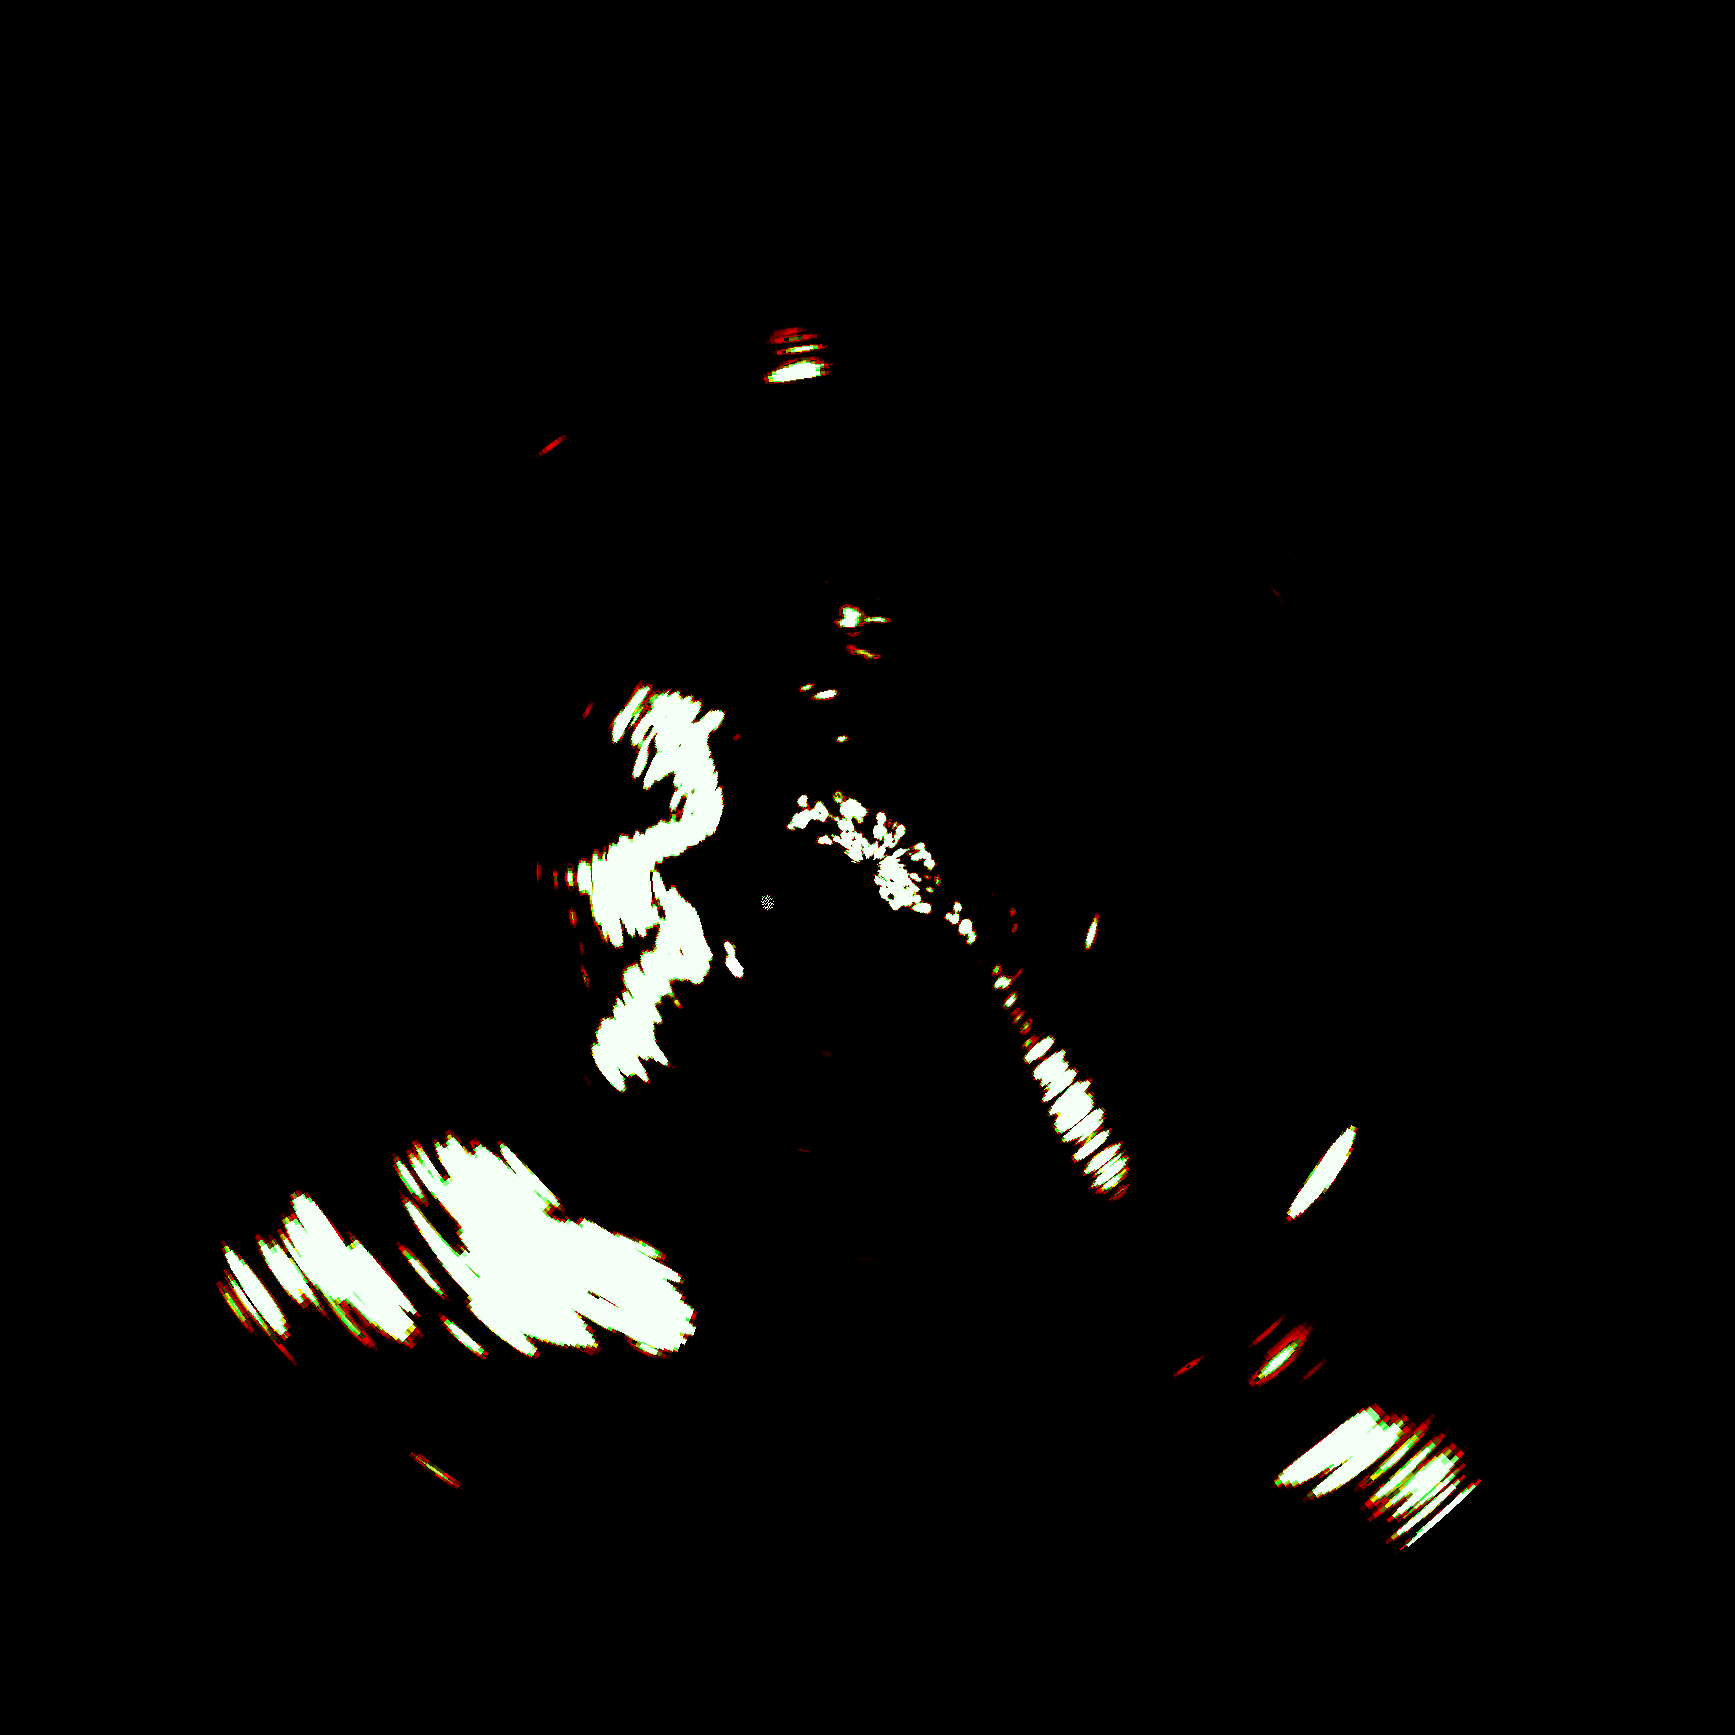
\includegraphics[width=\linewidth]{grayscale_frame.png}
    \caption{Raw composite}
\end{subcaptionblock}
\hfill
\begin{subcaptionblock}{0.32\columnwidth}
    \centering
    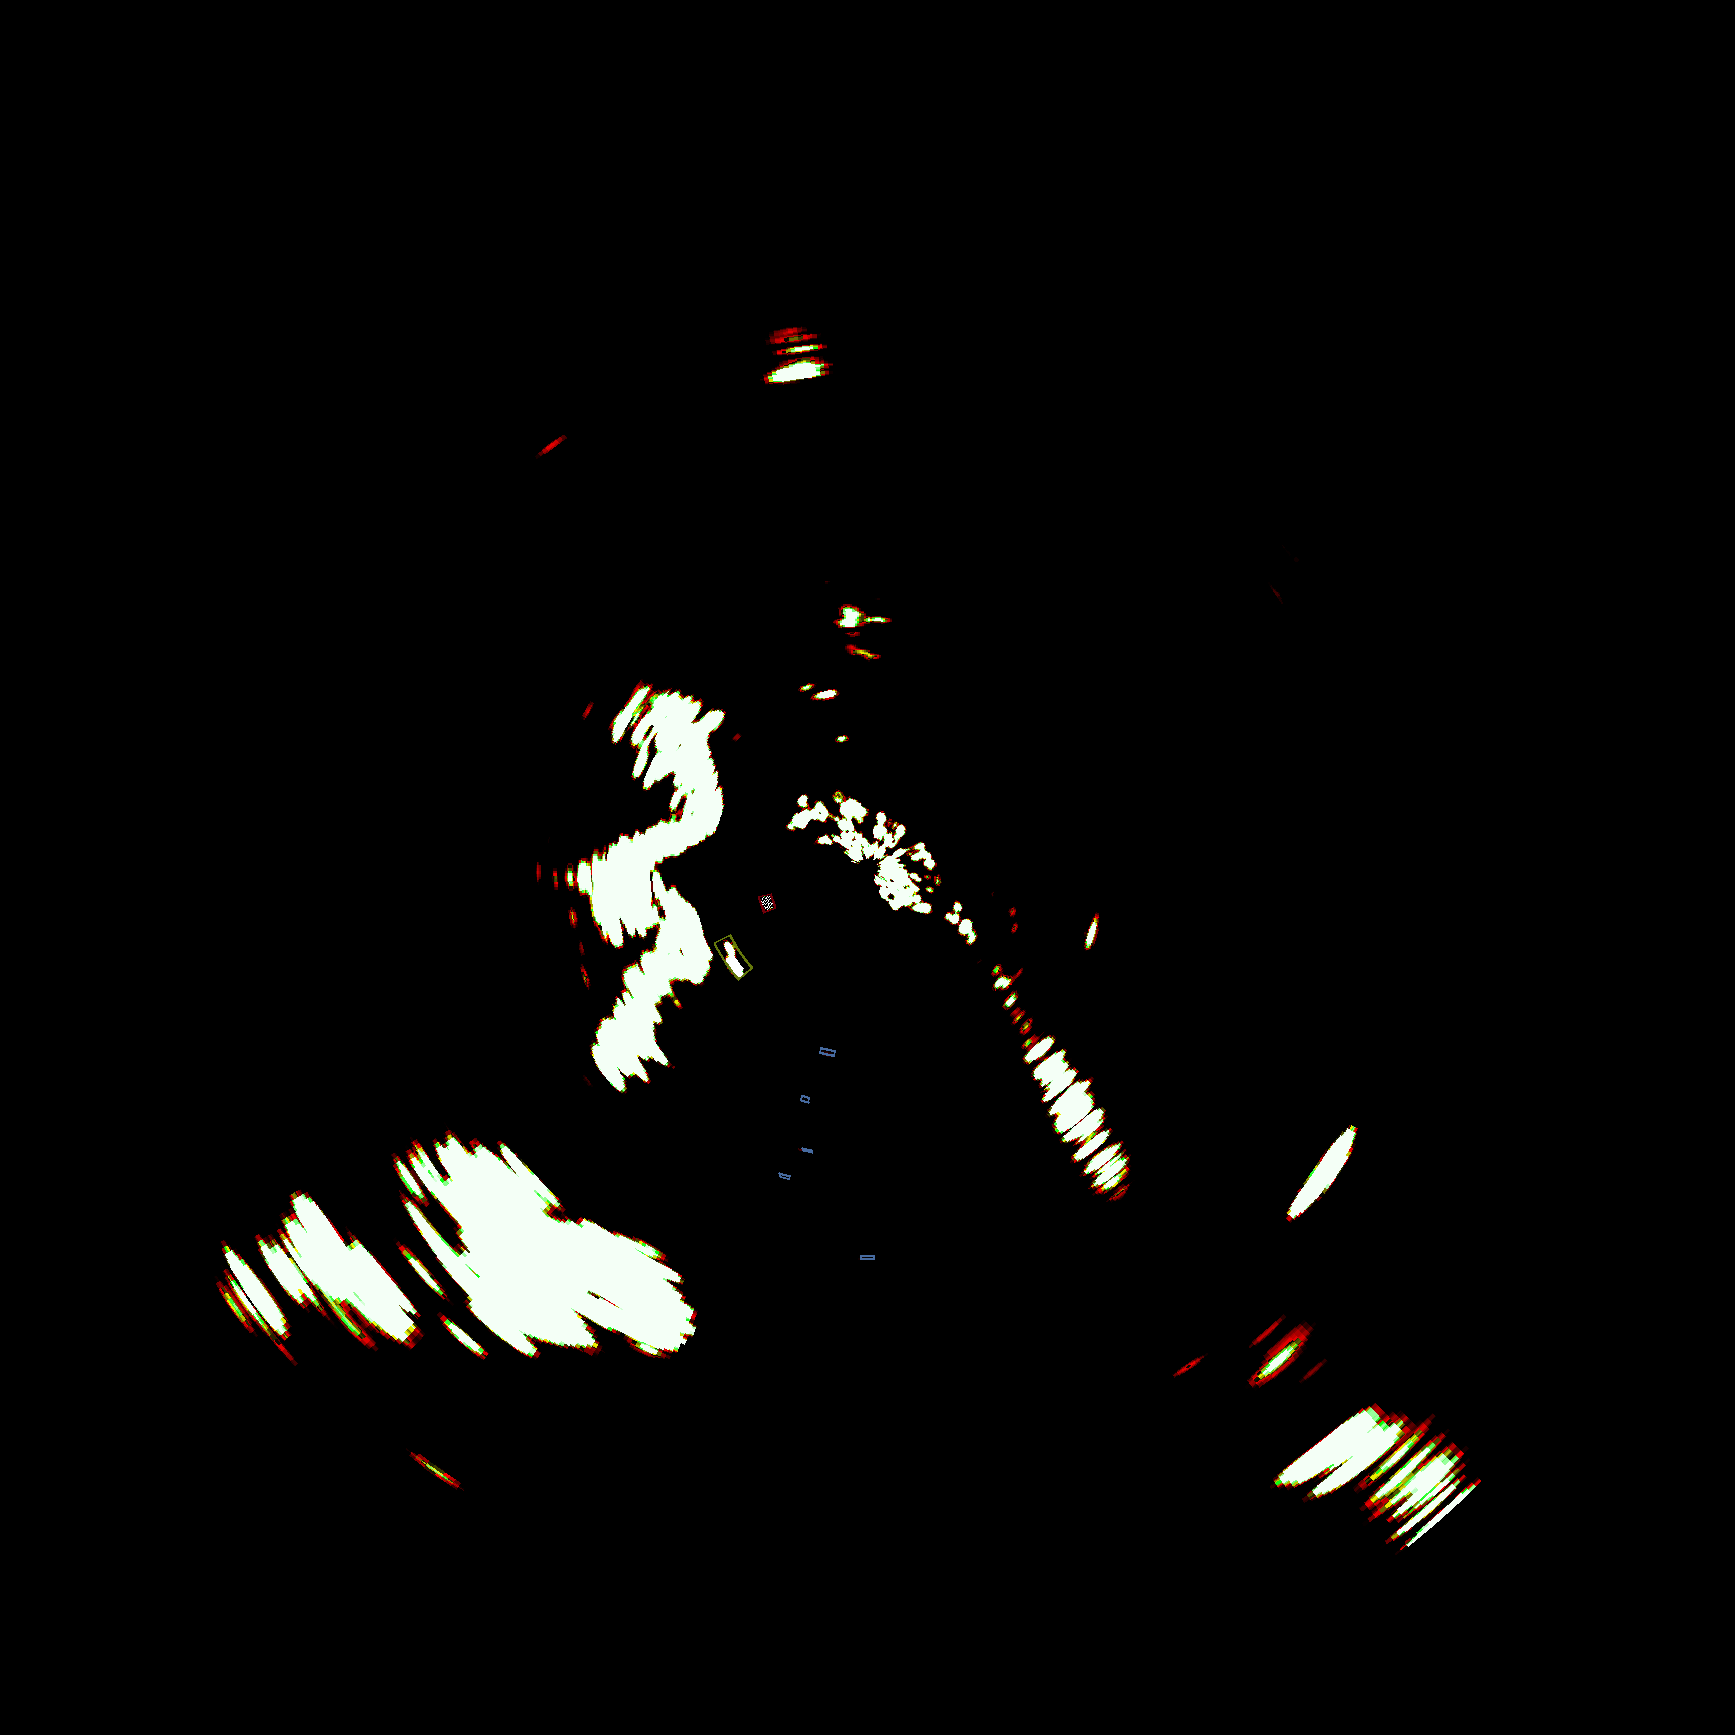
\includegraphics[width=\linewidth]{frame_with_boxes.png}
    \caption{With YOLO labels}
\end{subcaptionblock}
\hfill
\begin{subcaptionblock}{0.32\columnwidth}
    \centering
    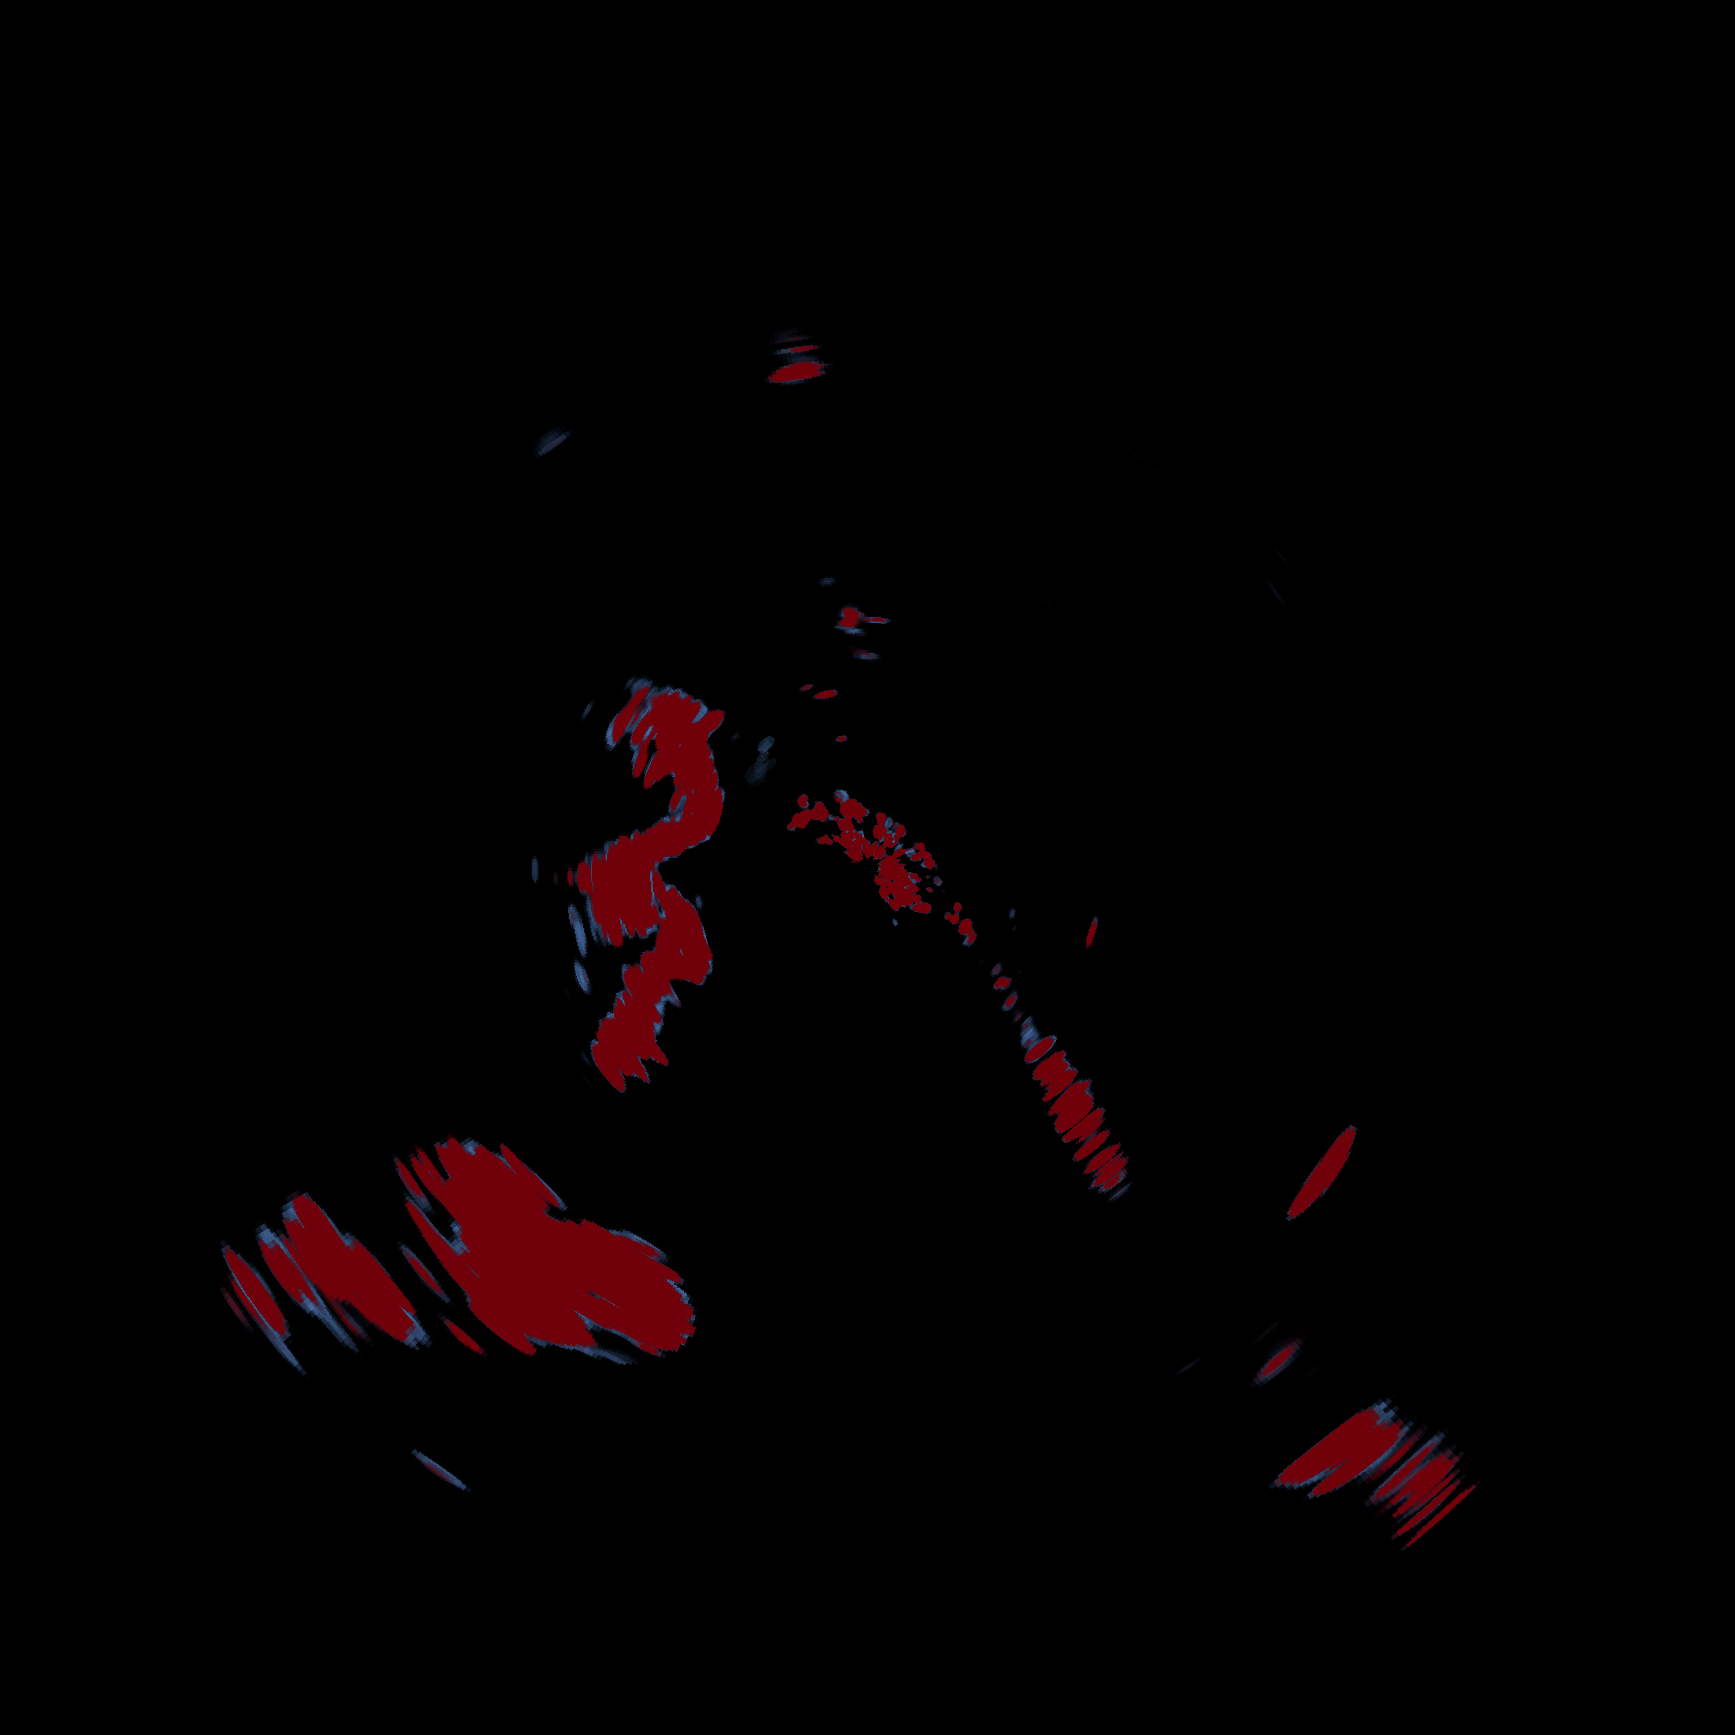
\includegraphics[width=\linewidth]{echo_trails.png}
    \caption{Echo trails}
\end{subcaptionblock}
\caption{Tier~3 compositor output. (a)~Composited radar frame in Cartesian projection. (b)~Same frame with YOLO bounding-box labels overlaid. (c)~Echo-trail persistence display.}
\label{fig:tier3_output}
\end{figure}

Figure~\ref{fig:intensity_profiles} demonstrates the four intensity profile types applied to a composited object over a 200-frame sequence.

\begin{figure}[htb]
\centering
\begin{subcaptionblock}{0.24\columnwidth}
    \centering
    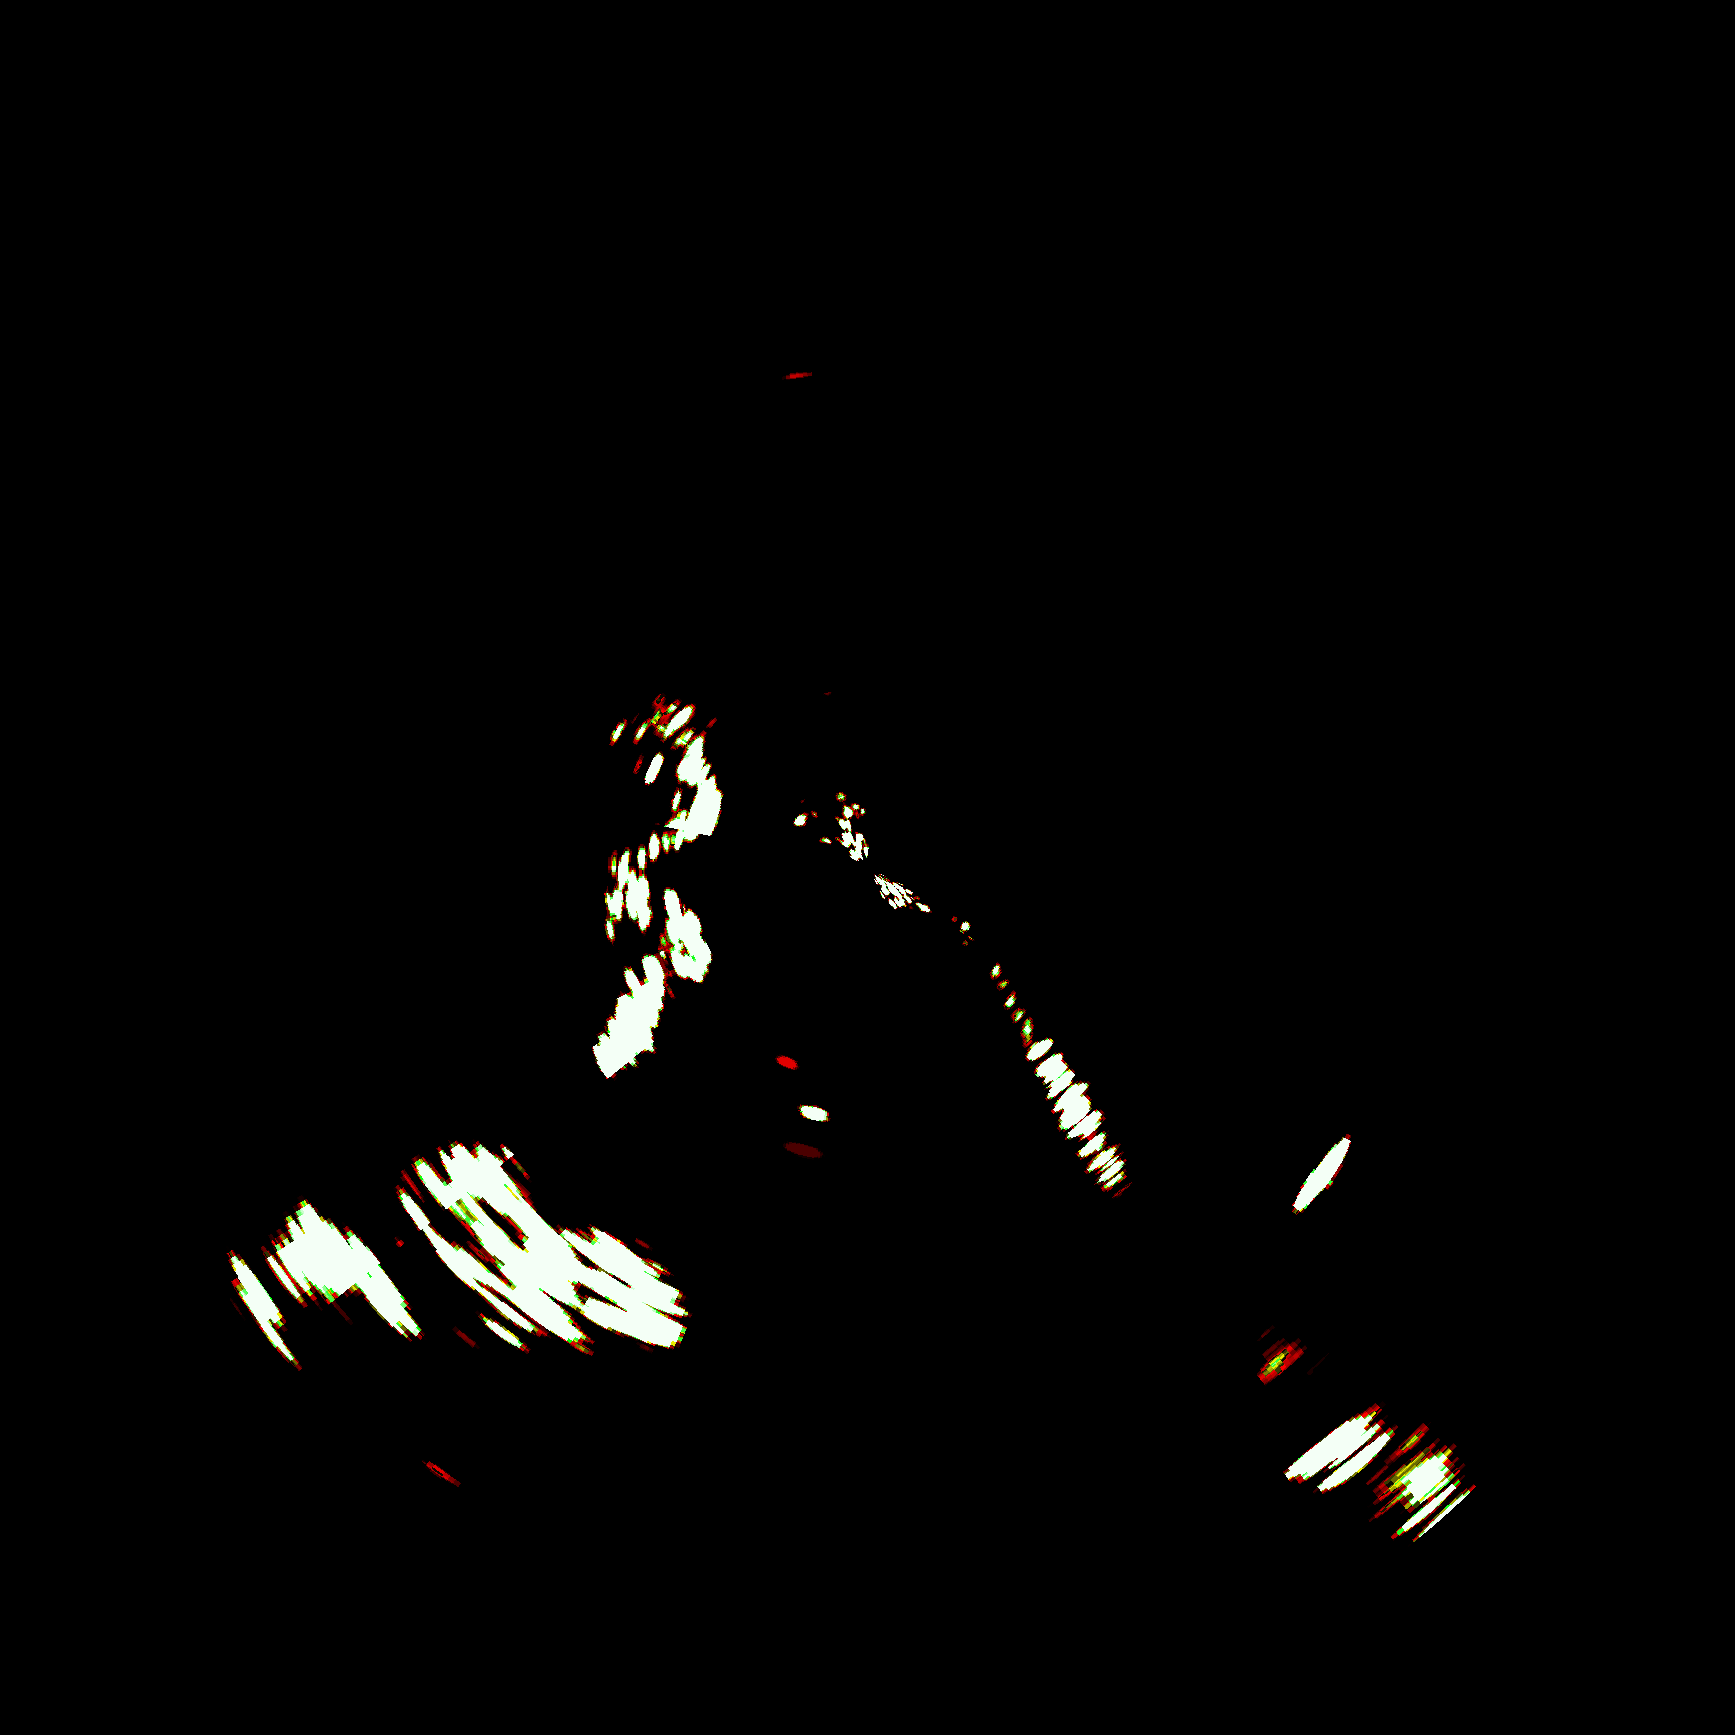
\includegraphics[width=\linewidth]{intensity_constant.png}
    \caption{Constant}
\end{subcaptionblock}
\hfill
\begin{subcaptionblock}{0.24\columnwidth}
    \centering
    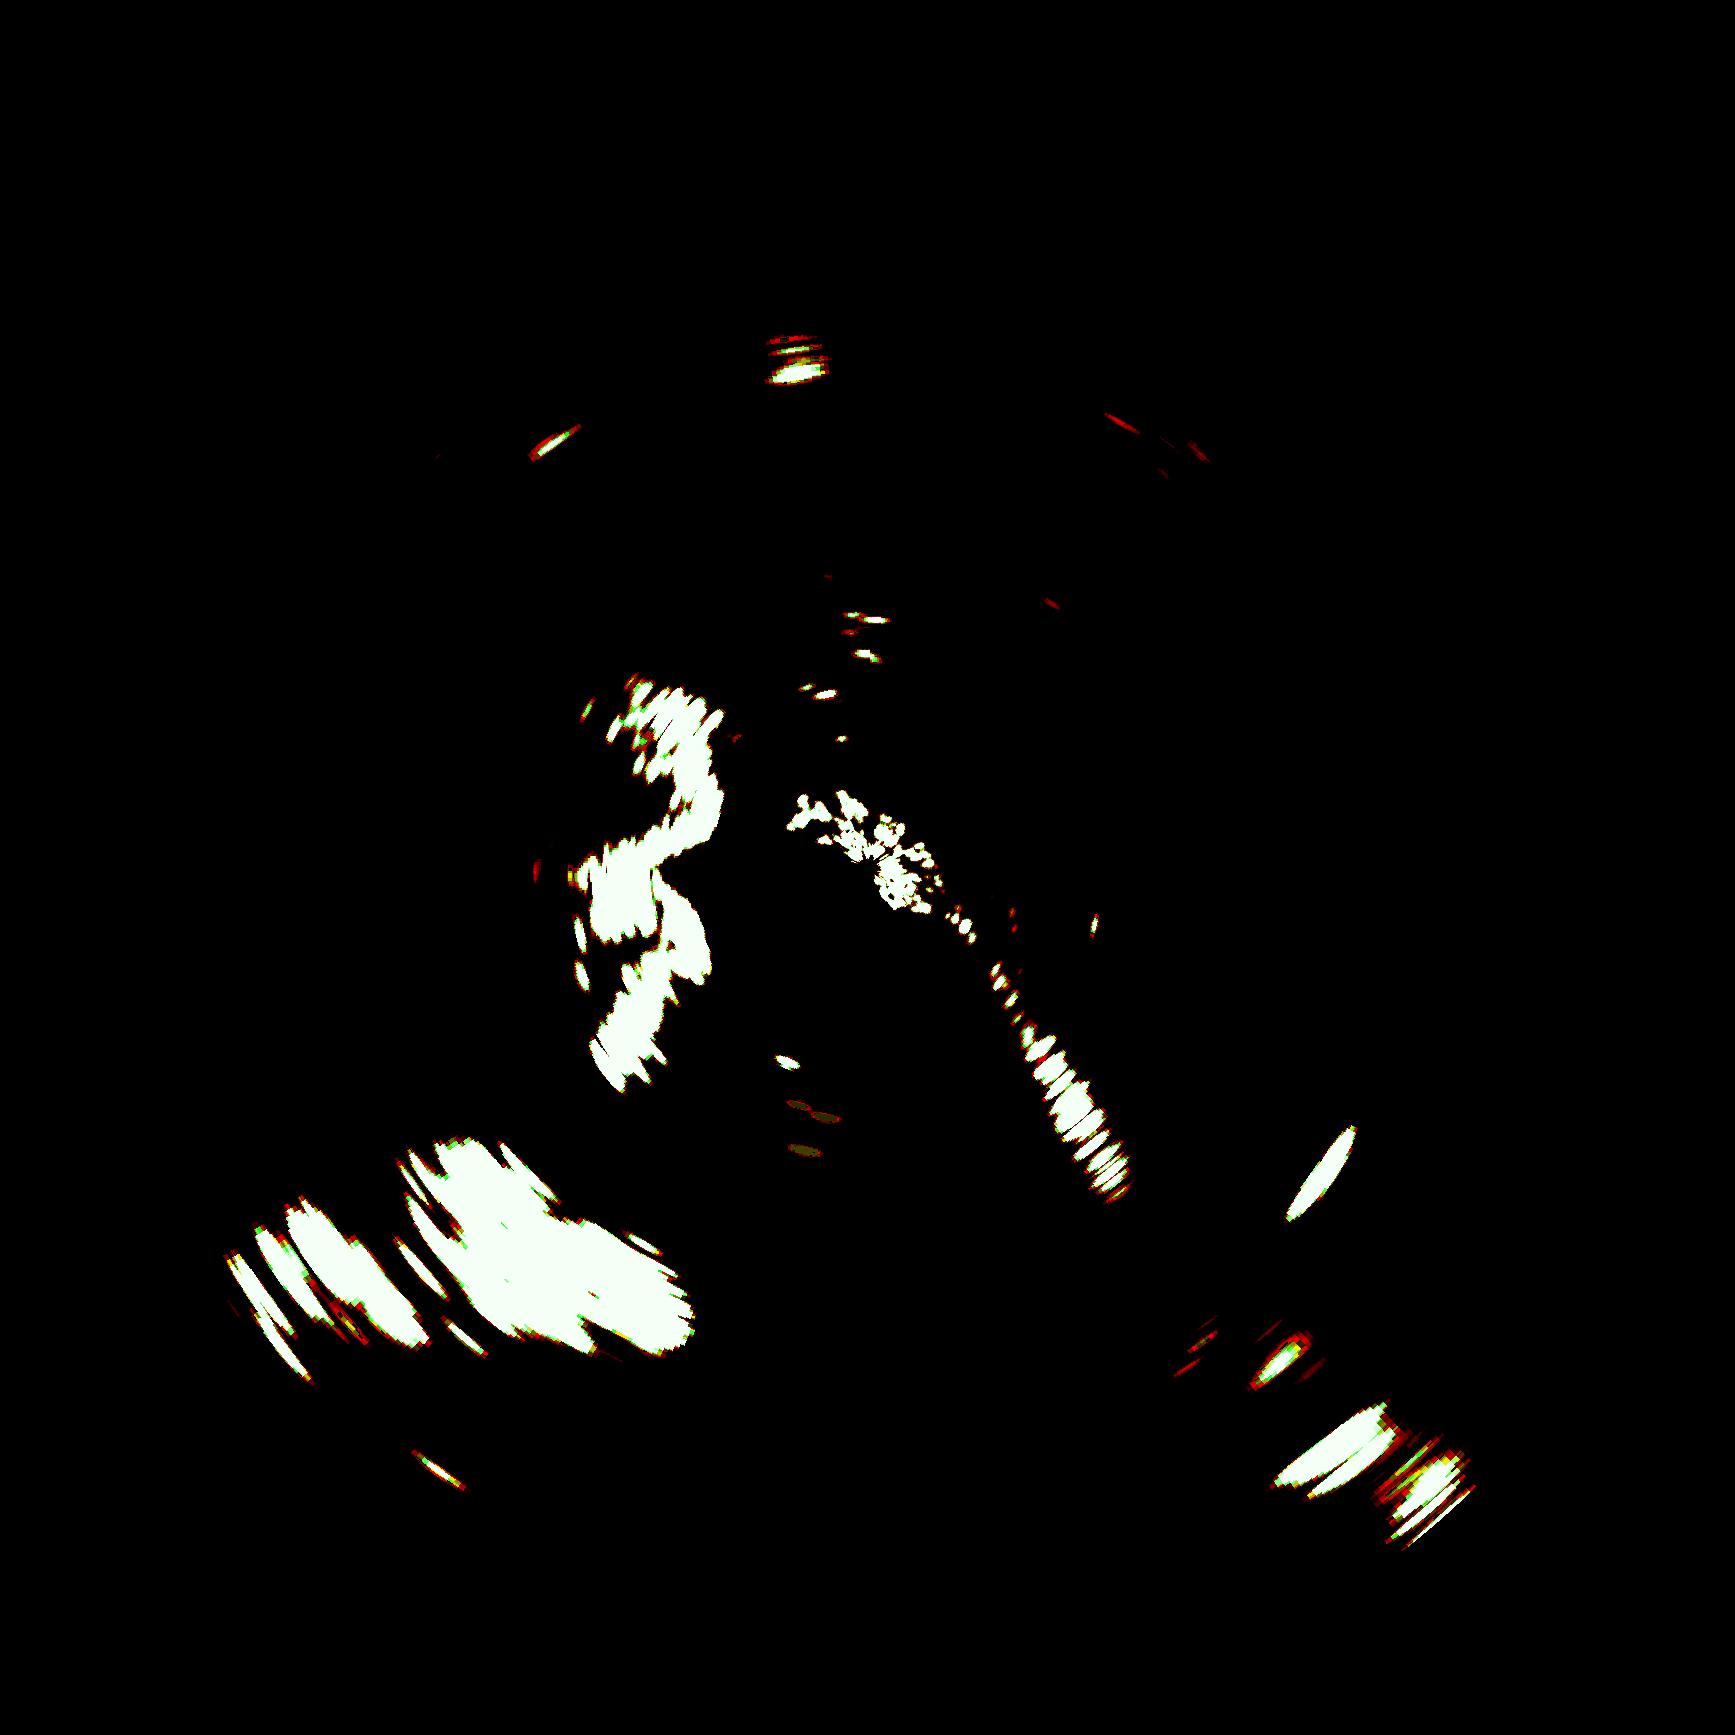
\includegraphics[width=\linewidth]{intensity_ramp.png}
    \caption{Ramp}
\end{subcaptionblock}
\hfill
\begin{subcaptionblock}{0.24\columnwidth}
    \centering
    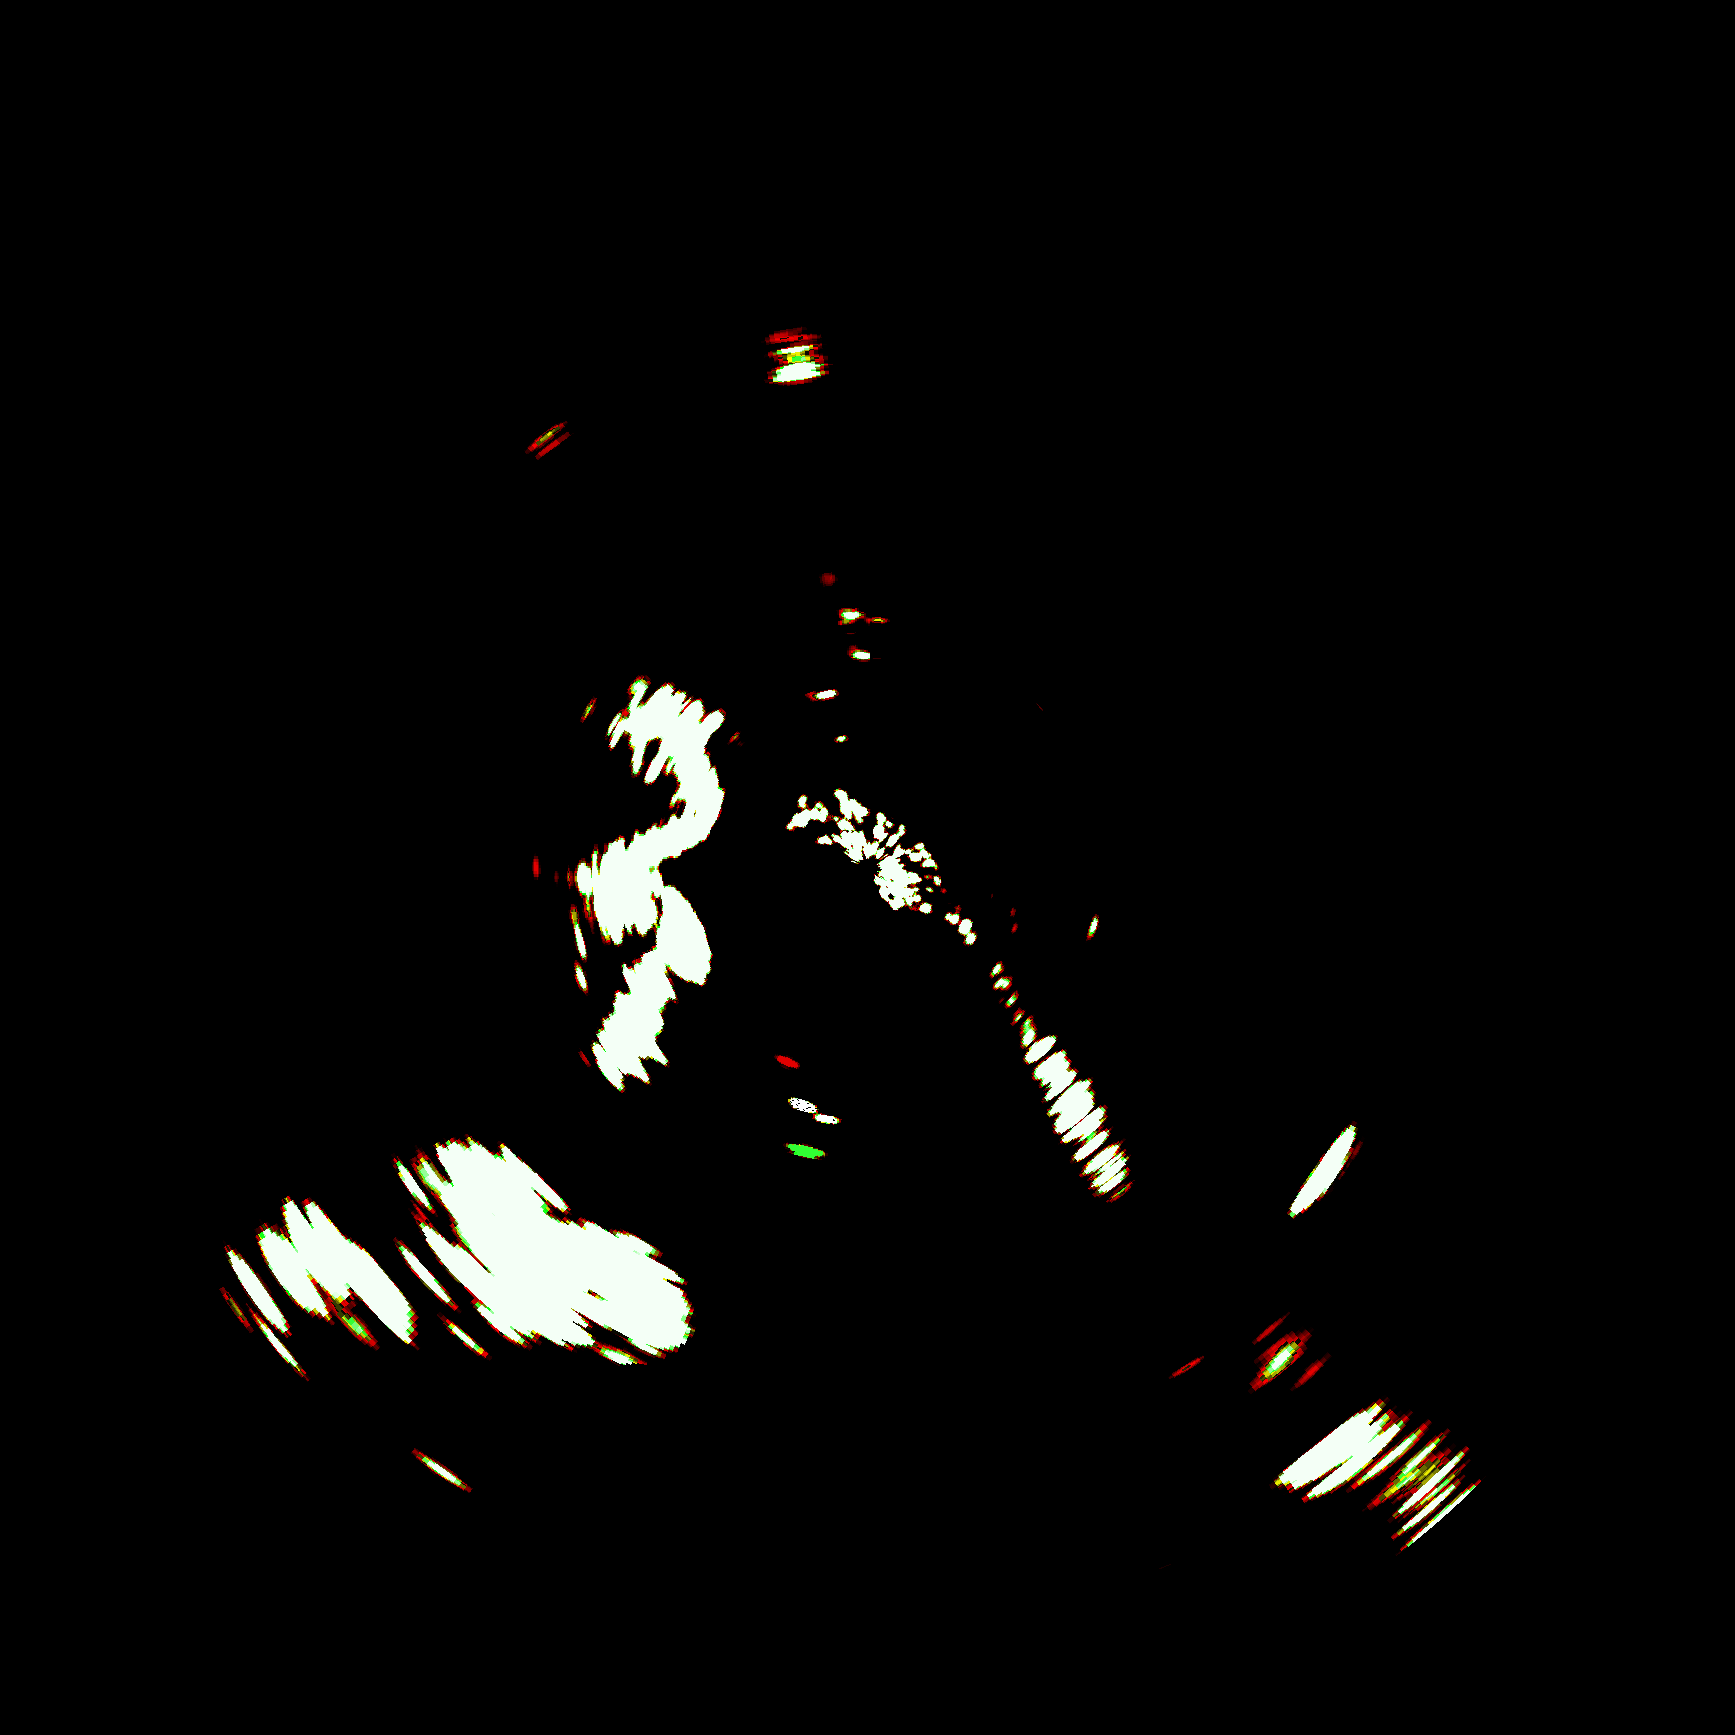
\includegraphics[width=\linewidth]{intensity_sine.png}
    \caption{Sinusoidal}
\end{subcaptionblock}
\hfill
\begin{subcaptionblock}{0.24\columnwidth}
    \centering
    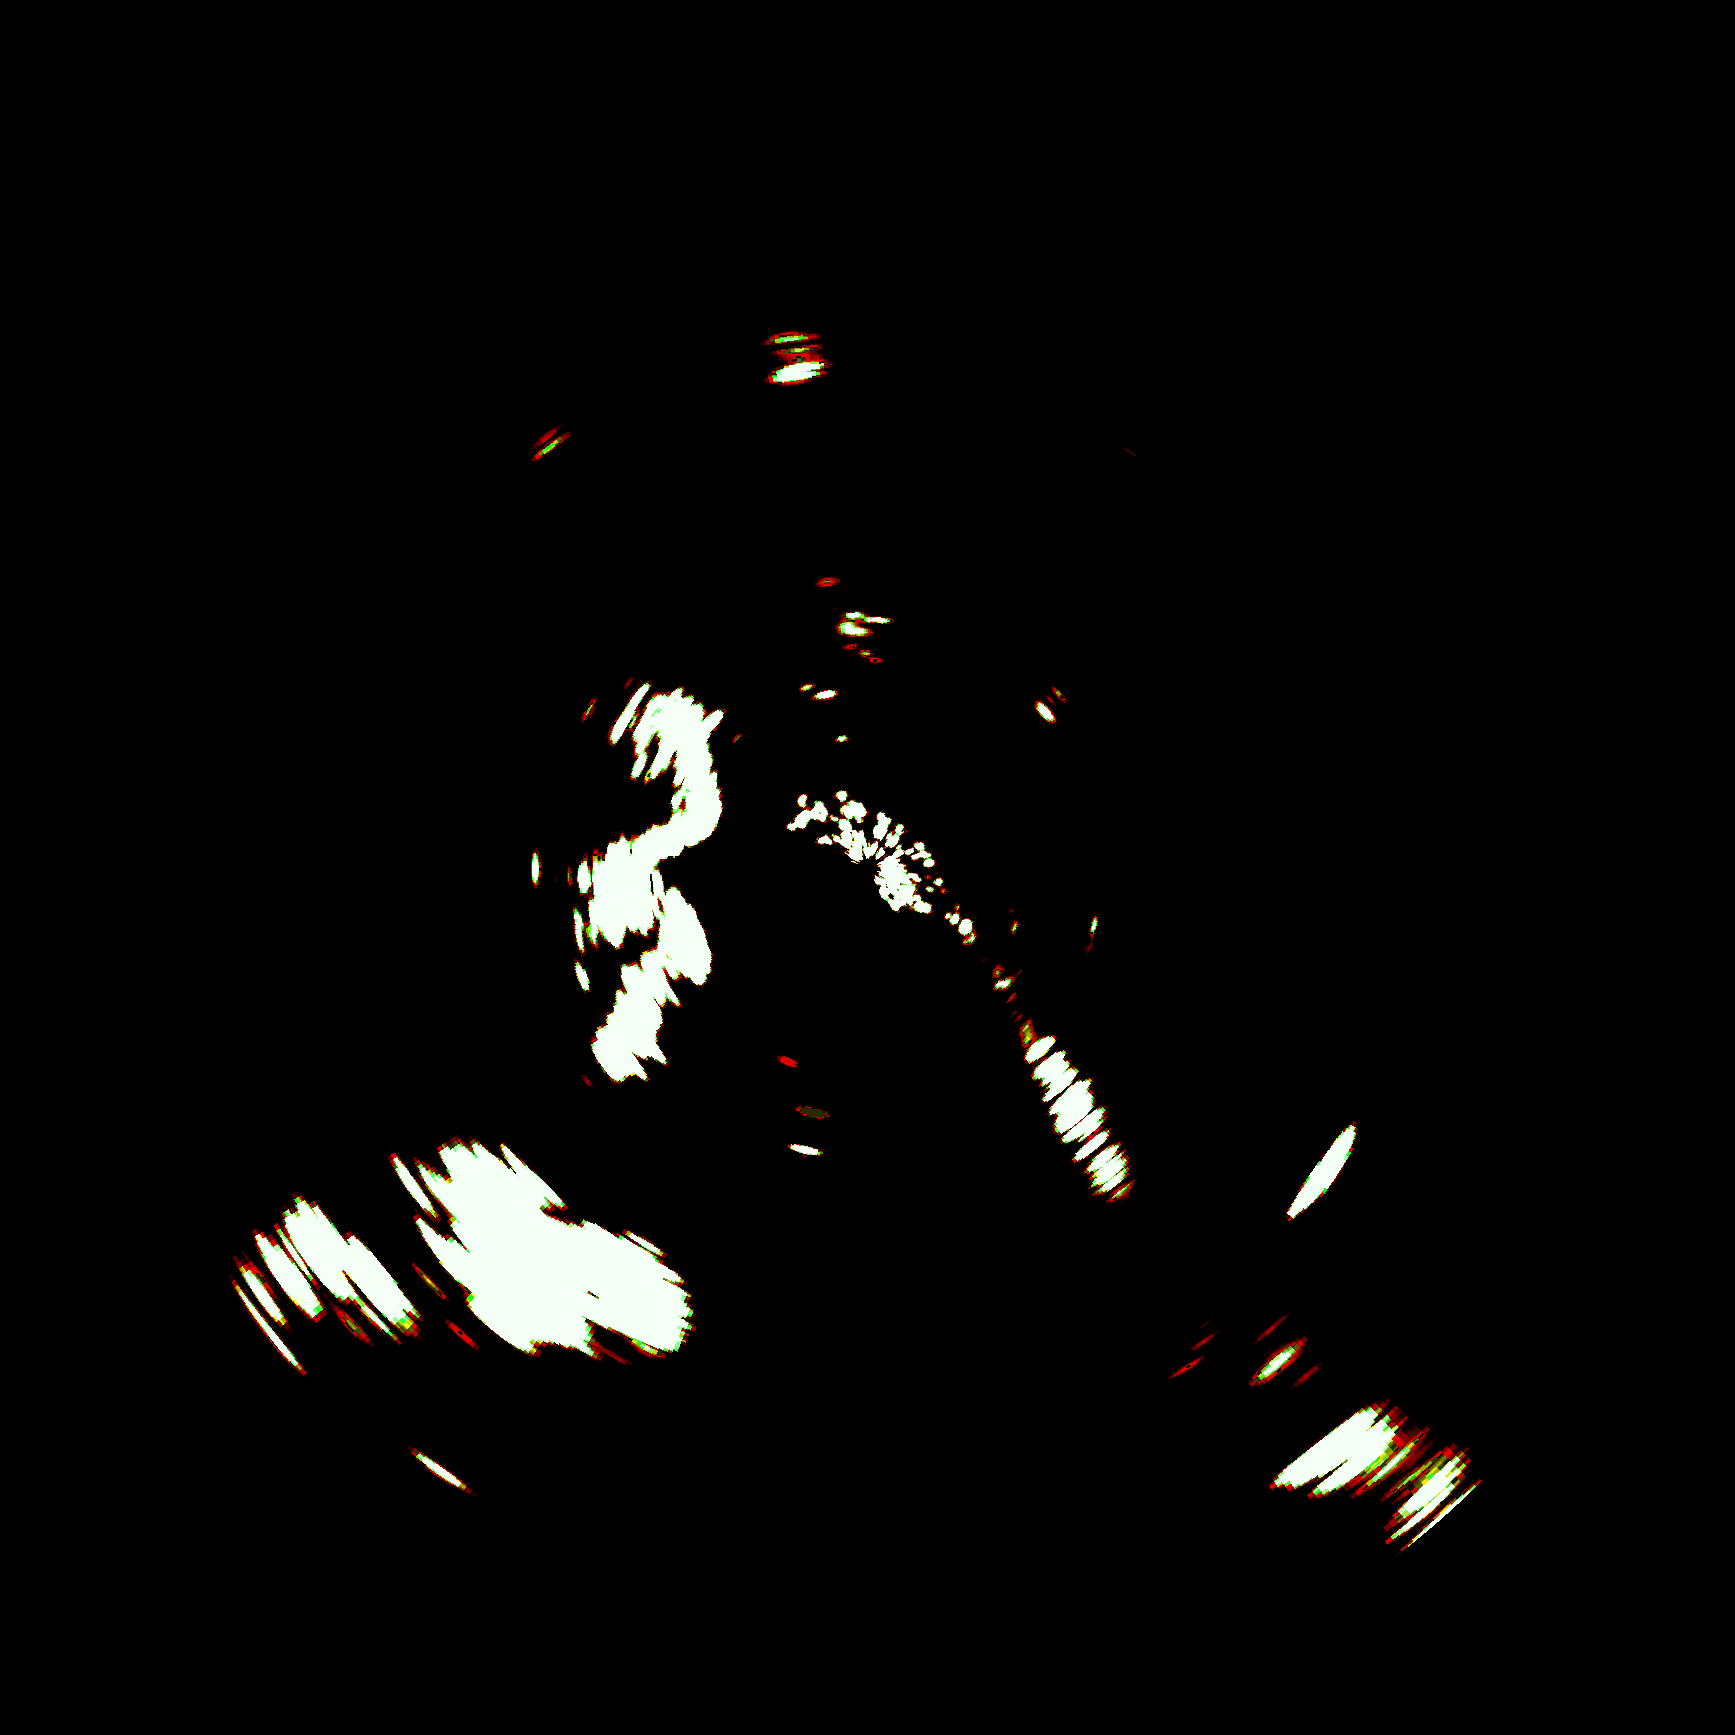
\includegraphics[width=\linewidth]{intensity_custom.png}
    \caption{Custom}
\end{subcaptionblock}
\caption{Intensity profile types. Each profile modulates the echo strength of a composited object over time, enabling simulation of fading, approach/departure, and arbitrary intensity patterns.}
\label{fig:intensity_profiles}
\end{figure}

% ============================================================================
%  SECTION 7: IMPLEMENTATION
% ============================================================================
\section{Implementation Details}\label{sec:implementation}

Table~\ref{tab:implementation} summarizes the software stack and computational performance for each tier.

\begin{table}[htb]
\centering
\caption{Implementation summary by tier.}
\label{tab:implementation}
\begin{tabular}{@{}lllll@{}}
\toprule
\textbf{Tier} & \textbf{Language} & \textbf{Key Libraries} & \textbf{Parallelism} & \textbf{Time/Frame} \\
\midrule
1 & Python & NumPy, SciPy, PyVista & Vectorized & Minutes \\
2 & Python & NumPy, SciPy & Vectorized & Seconds \\
3 & Python + Rust & Pillow, FFmpeg & Per-stage & Sub-second \\
\bottomrule
\end{tabular}
\end{table}

\subsection{Tier 1 Implementation}
The Tier~1 engine is implemented in Python with NumPy-vectorized array operations for the core computational loops. The M\"{o}ller-Trumbore ray-triangle intersection test operates on batched rays ($\sim$100{,}000 per azimuth step) against the full scene mesh. SciPy provides the FFT engine for pulse compression and the signal processing utilities for matched filtering. PyVista is used for 3D visualization and mesh manipulation during scene construction. Scene configurations are specified in YAML files, enabling reproducible simulation runs without code modification.

\subsection{Tier 2 Implementation}
Tier~2 leverages SciPy's special functions (modified Bessel functions for K-distribution sampling, gamma distributions for texture generation) and NumPy's random number generators with configurable seeds for reproducibility. The entire $720 \times 868$ polar grid is populated in a single vectorized pass per frame. Spatial correlation is applied via convolution, and the multipath propagation factor is computed analytically for each range bin.

\subsection{Tier 3 Implementation}
The extraction tools (annotator, scene extractor, land extractor) are implemented in Rust for performance-critical I/O operations on large CSV files (868 range bins per azimuth line, 720 lines per frame). The synthesis pipeline is implemented in Python, with each of the six stages independently configurable. Scene descriptions are specified in YAML, including object counts, motion models, intensity profiles, and output format selections.

\subsection{Configuration System}
All three tiers consume YAML configuration files that specify radar parameters, environment conditions, target properties, and output formats. A representative configuration for Tier~2 includes fields for simulation seed, radar RF parameters (frequency, power, antenna height, gain, beamwidth), environment conditions (sea state, wind speed, rain rate, ducting), target distributions (count, range, RCS, Swerling case), and output format selections (polar CSV, Cartesian PNG, YOLO labels, echo trails, video).

% ============================================================================
%  SECTION 8: RESULTS AND VALIDATION
% ============================================================================
\section{Results and Validation}\label{sec:results}

\subsection{Tier 1: Corner Reflector and Pulse Compression}
The Tier~1 pipeline was validated using a trihedral corner reflector with side length $a = 76.2$~mm (3~inches). The analytical RCS for a trihedral reflector at normal incidence is
\begin{equation}\label{eq:corner_rcs}
\sigma_{\mathrm{tri}} = \frac{12\pi a^4}{\lambda^2}.
\end{equation}
At $\lambda = 31.8$~mm, this yields $\sigma = 0.082$~m$^2$ ($-10.9$~dBsm). The PO simulation produced a value consistent with the analytical prediction, as shown in Fig.~\ref{fig:corner_reflector}.

Pulse compression was validated by measuring the compression gain and sidelobe levels. The matched filter achieves a theoretical compression gain of $10\log_{10}(BT) = 10\log_{10}(500) = 27.0$~dB. The measured 3-dB mainlobe width after compression corresponds to a range resolution of approximately $c/(2B) = 3$~m. With Taylor windowing, the first sidelobe is suppressed to approximately $-35$~dB relative to the mainlobe peak, at the cost of a modest 15\% mainlobe broadening.

\subsection{Tier 1: PPI Output Quality}
The full Tier~1 pipeline produces plan-position indicator (PPI) images that capture the essential phenomenology of a real X-band marine radar, including range-dependent clutter fall-off, shadow regions behind terrain, and distinct target returns. Figure~\ref{fig:harbor_ppi} shows a harbor scene with coastline returns, and Figure~\ref{fig:combined_ppi} shows a combined simulation with multiple targets.

\begin{figure}[htb]
\centering
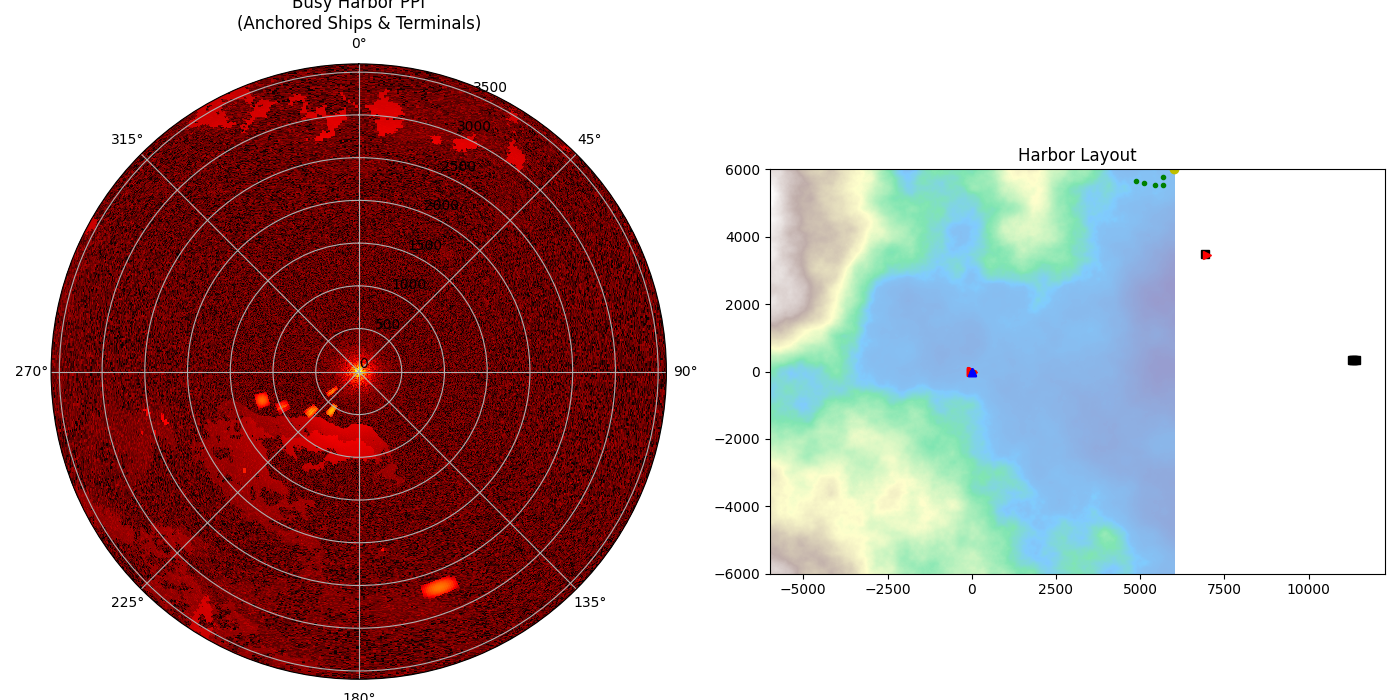
\includegraphics[width=0.9\columnwidth]{harbor_demo.png}
\caption{Tier~1 PPI output for a harbor scene. Coastline returns, pier structures, and moored vessels are visible with realistic range-dependent intensity.}
\label{fig:harbor_ppi}
\end{figure}

\begin{figure}[htb]
\centering
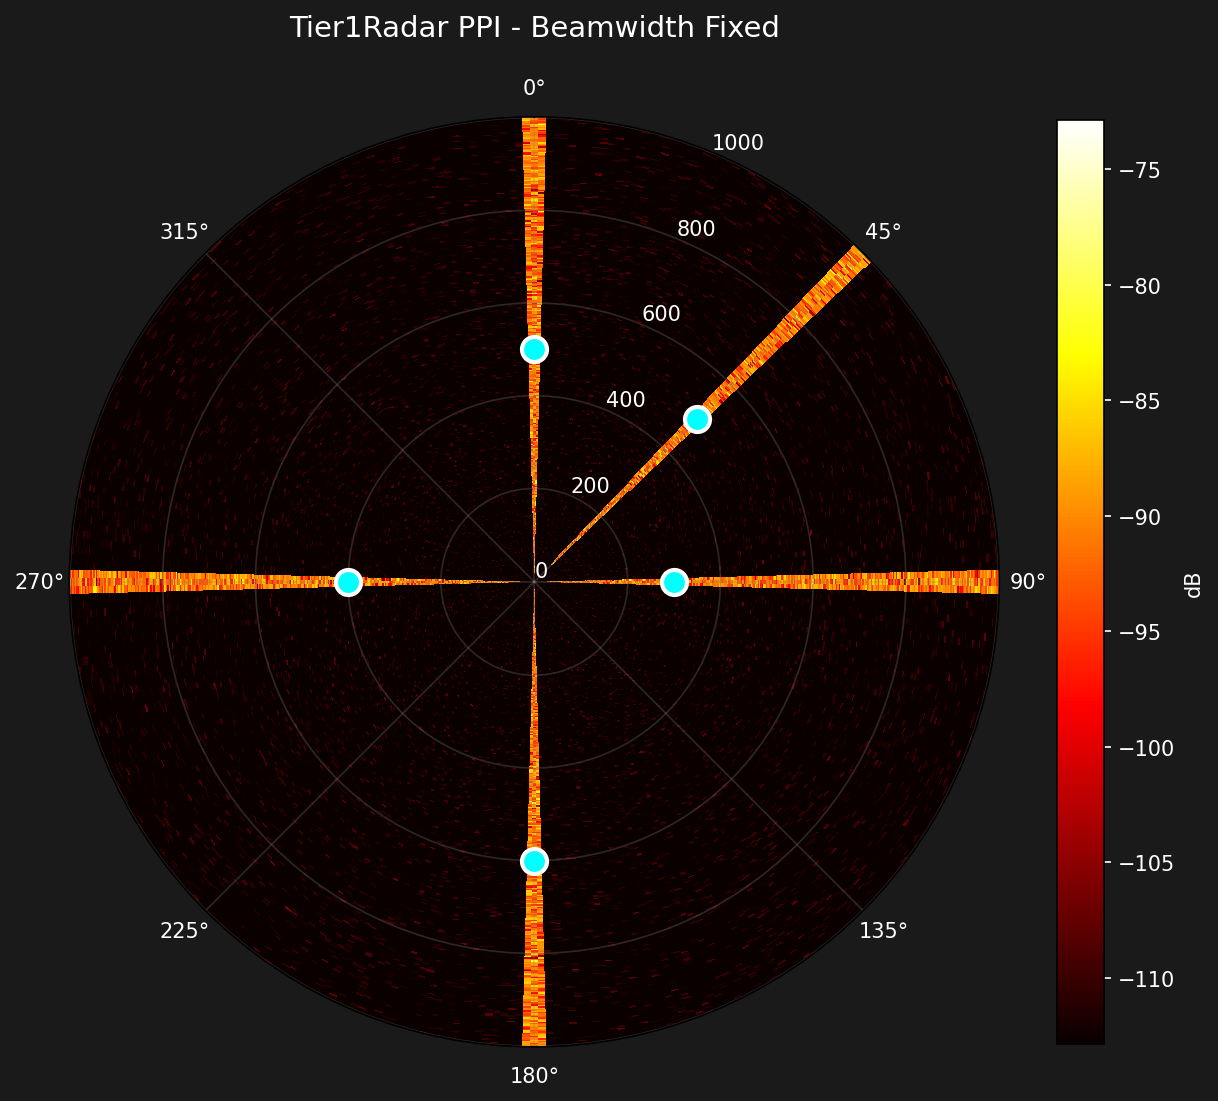
\includegraphics[width=0.9\columnwidth]{demo_ppi.png}
\caption{Tier~1 combined-simulation PPI output with terrain, sea surface, and multiple targets at varying ranges.}
\label{fig:combined_ppi}
\end{figure}

\subsection{Tier 2: Clutter Statistics}
The K-distribution clutter generator was validated by comparing the empirical histogram of $10^5$ generated samples against the theoretical PDF of Eq.~\eqref{eq:kdist} for representative shape parameters. The generated samples match the theoretical distribution across the full dynamic range, including the heavy-tail behavior at low shape parameters ($\nu < 1$) characteristic of high sea states. Figure~\ref{fig:kdist_validation} shows this comparison for sea state~4 ($\nu = 2.0$).

\begin{figure}[htb]
\centering
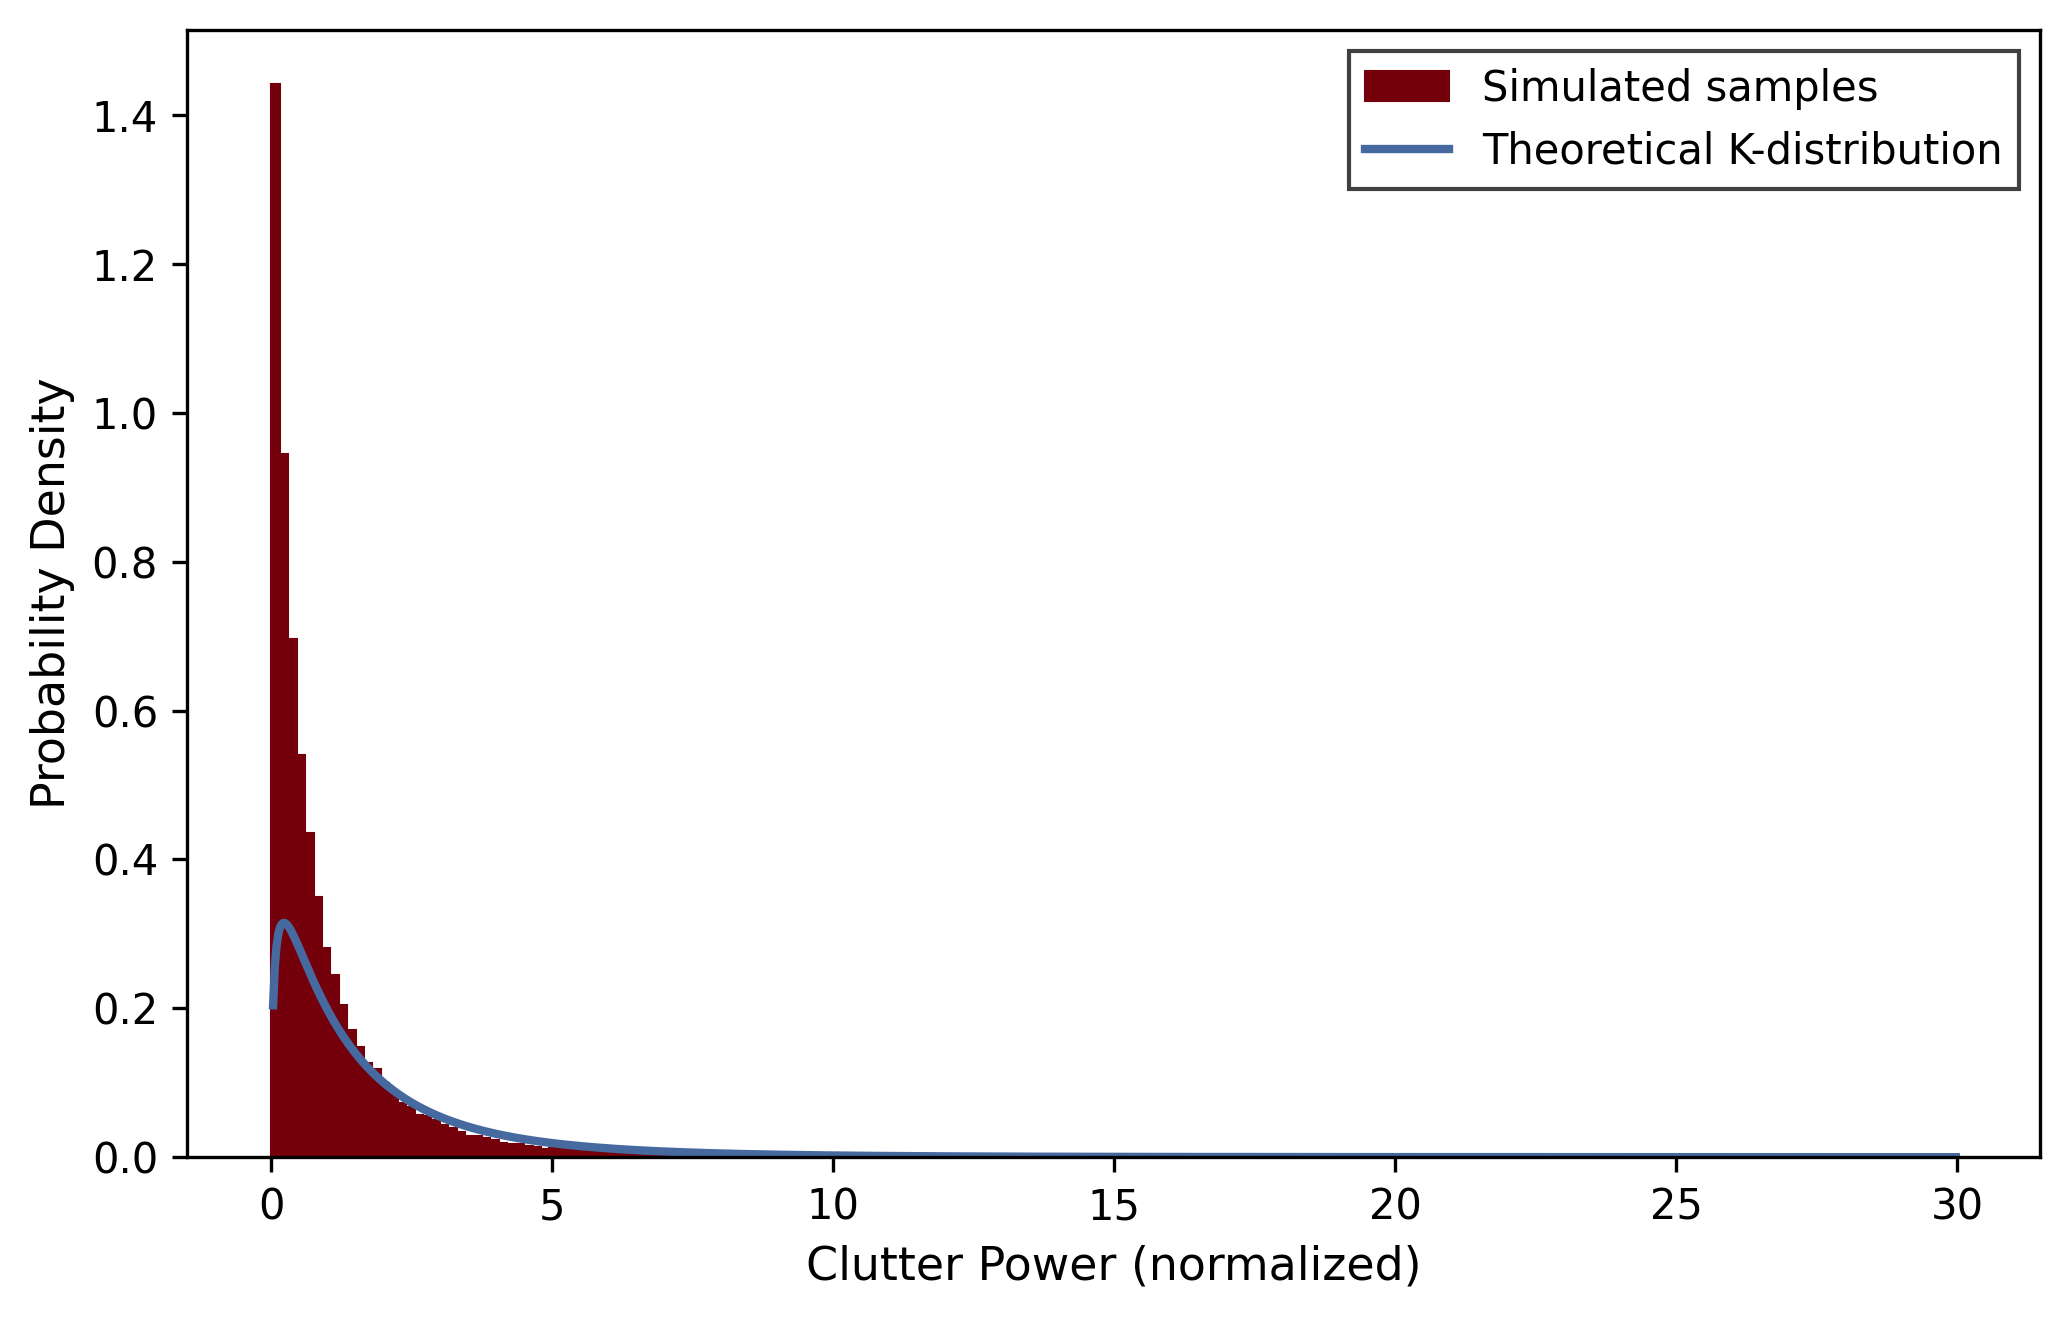
\includegraphics[width=0.9\columnwidth]{kdist_validation.png}
\caption{K-distribution clutter validation: empirical histogram of $10^5$ generated samples vs.\ theoretical PDF for sea state~4 ($\nu = 2.0$, $\mu = 5\times10^{-10}$).}
\label{fig:kdist_validation}
\end{figure}

\subsection{Tier 2: Swerling Model Comparison}
Figure~\ref{fig:swerling_pdfs} compares the theoretical PDFs for all five Swerling cases. Cases~1--2 (exponential) produce more frequent low-RCS realizations than cases~3--4 (chi-squared, 4 DOF), which are more concentrated around the mean. Case~0 is the non-fluctuating reference.

\begin{figure}[htb]
\centering
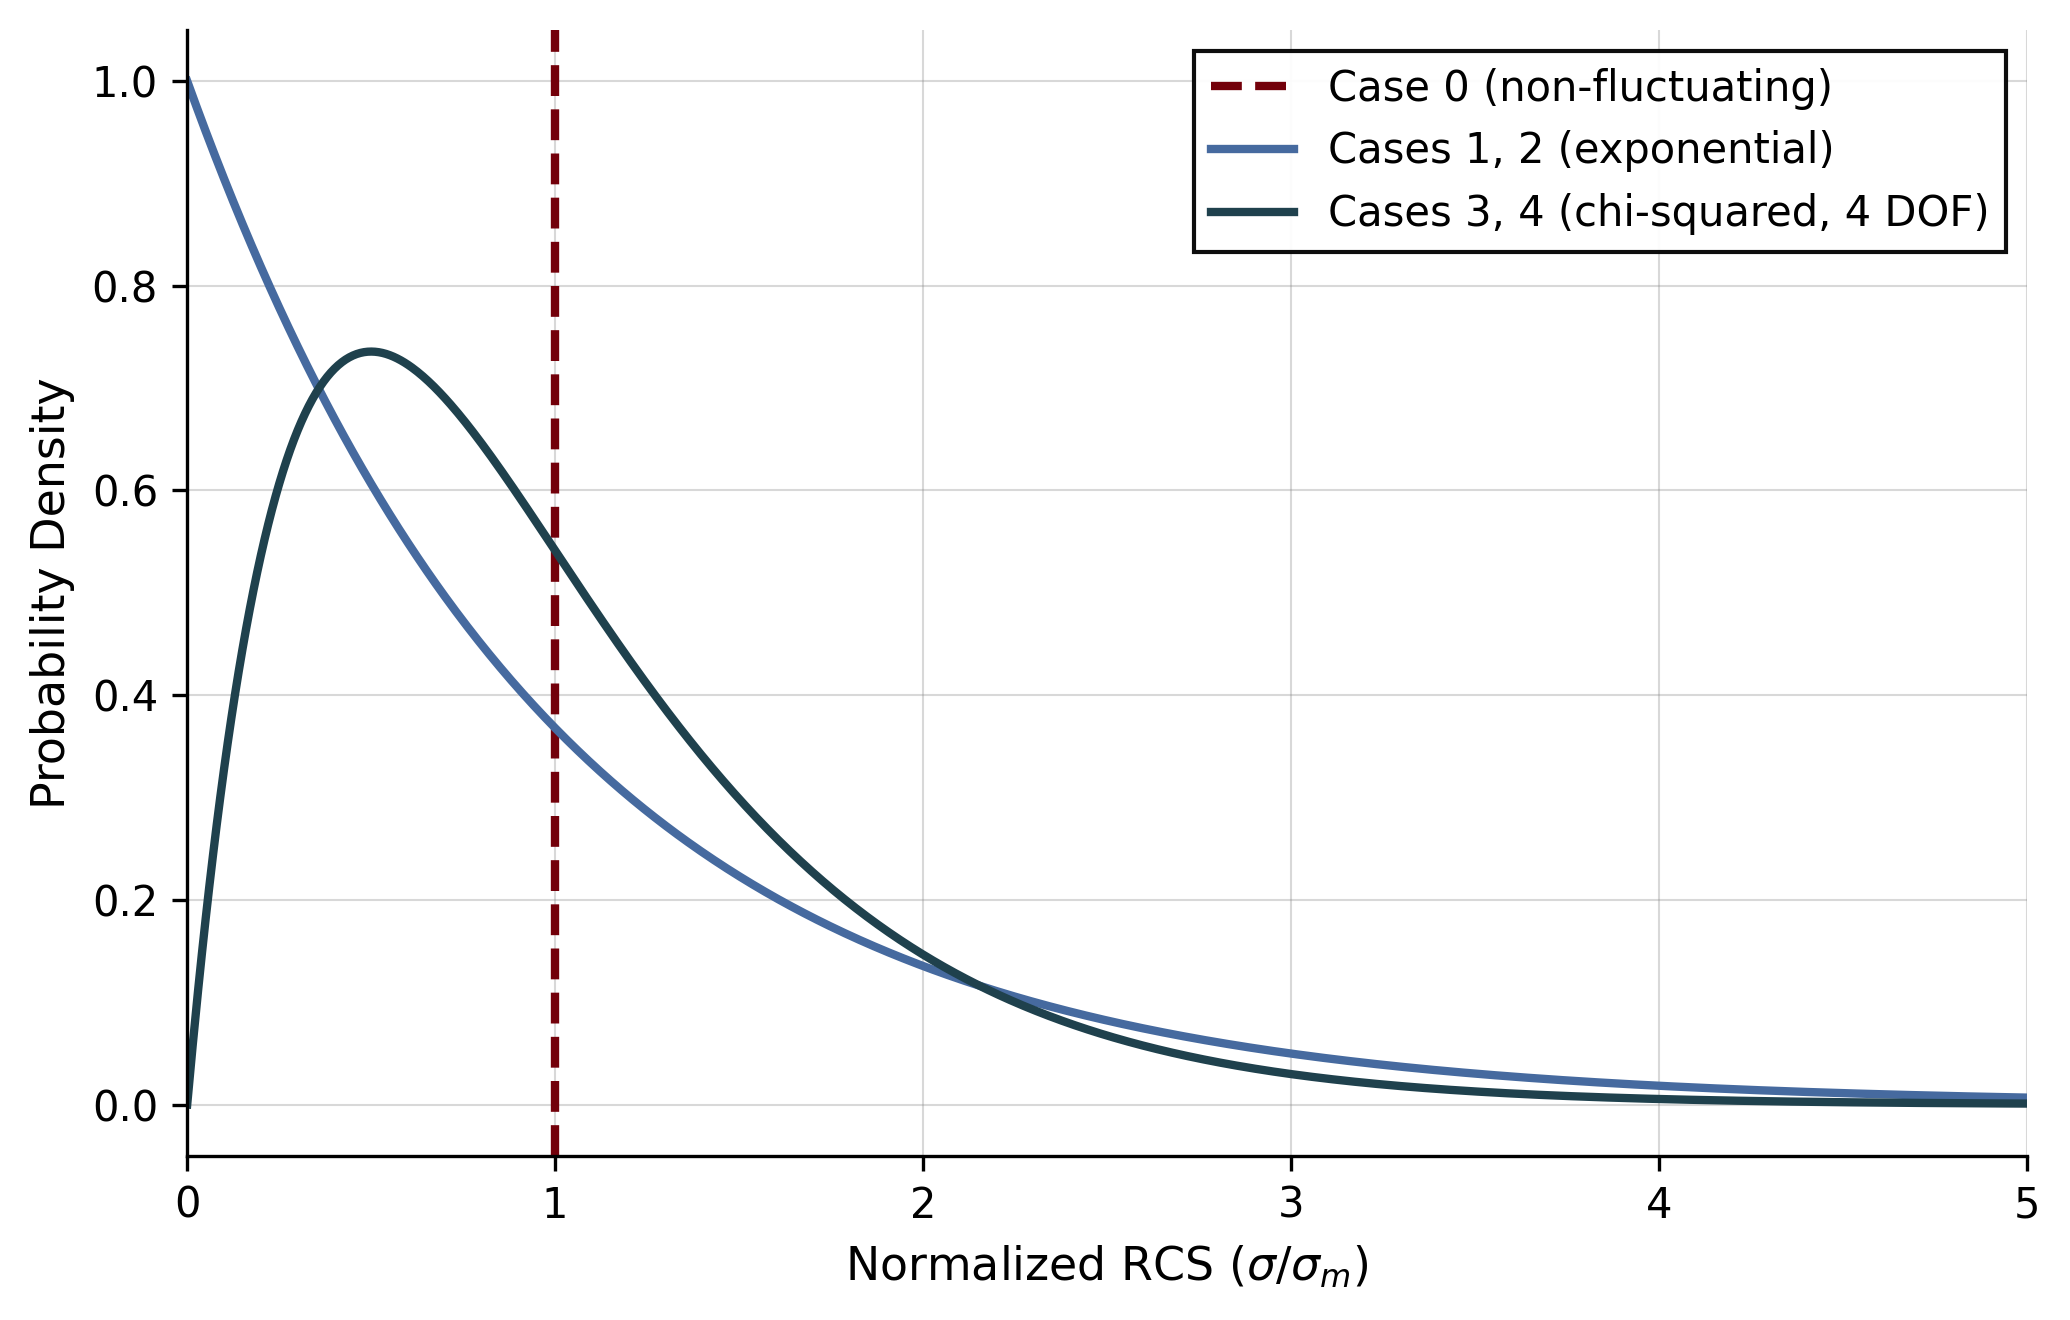
\includegraphics[width=0.9\columnwidth]{swerling_pdfs.png}
\caption{Swerling RCS fluctuation PDFs for all five cases with mean RCS $\sigma_m = 1$. Cases~1--2 follow an exponential distribution; cases~3--4 follow a chi-squared distribution with 4 degrees of freedom.}
\label{fig:swerling_pdfs}
\end{figure}

\subsection{Tier 2: Multipath Propagation Factor}
Figure~\ref{fig:multipath_factor} shows the two-ray propagation factor $F^4$ as a function of range for representative antenna and target heights. The characteristic lobing pattern, with deep nulls at ranges where the direct and reflected paths cancel and enhancement peaks where they add constructively, is evident.

\begin{figure}[htb]
\centering
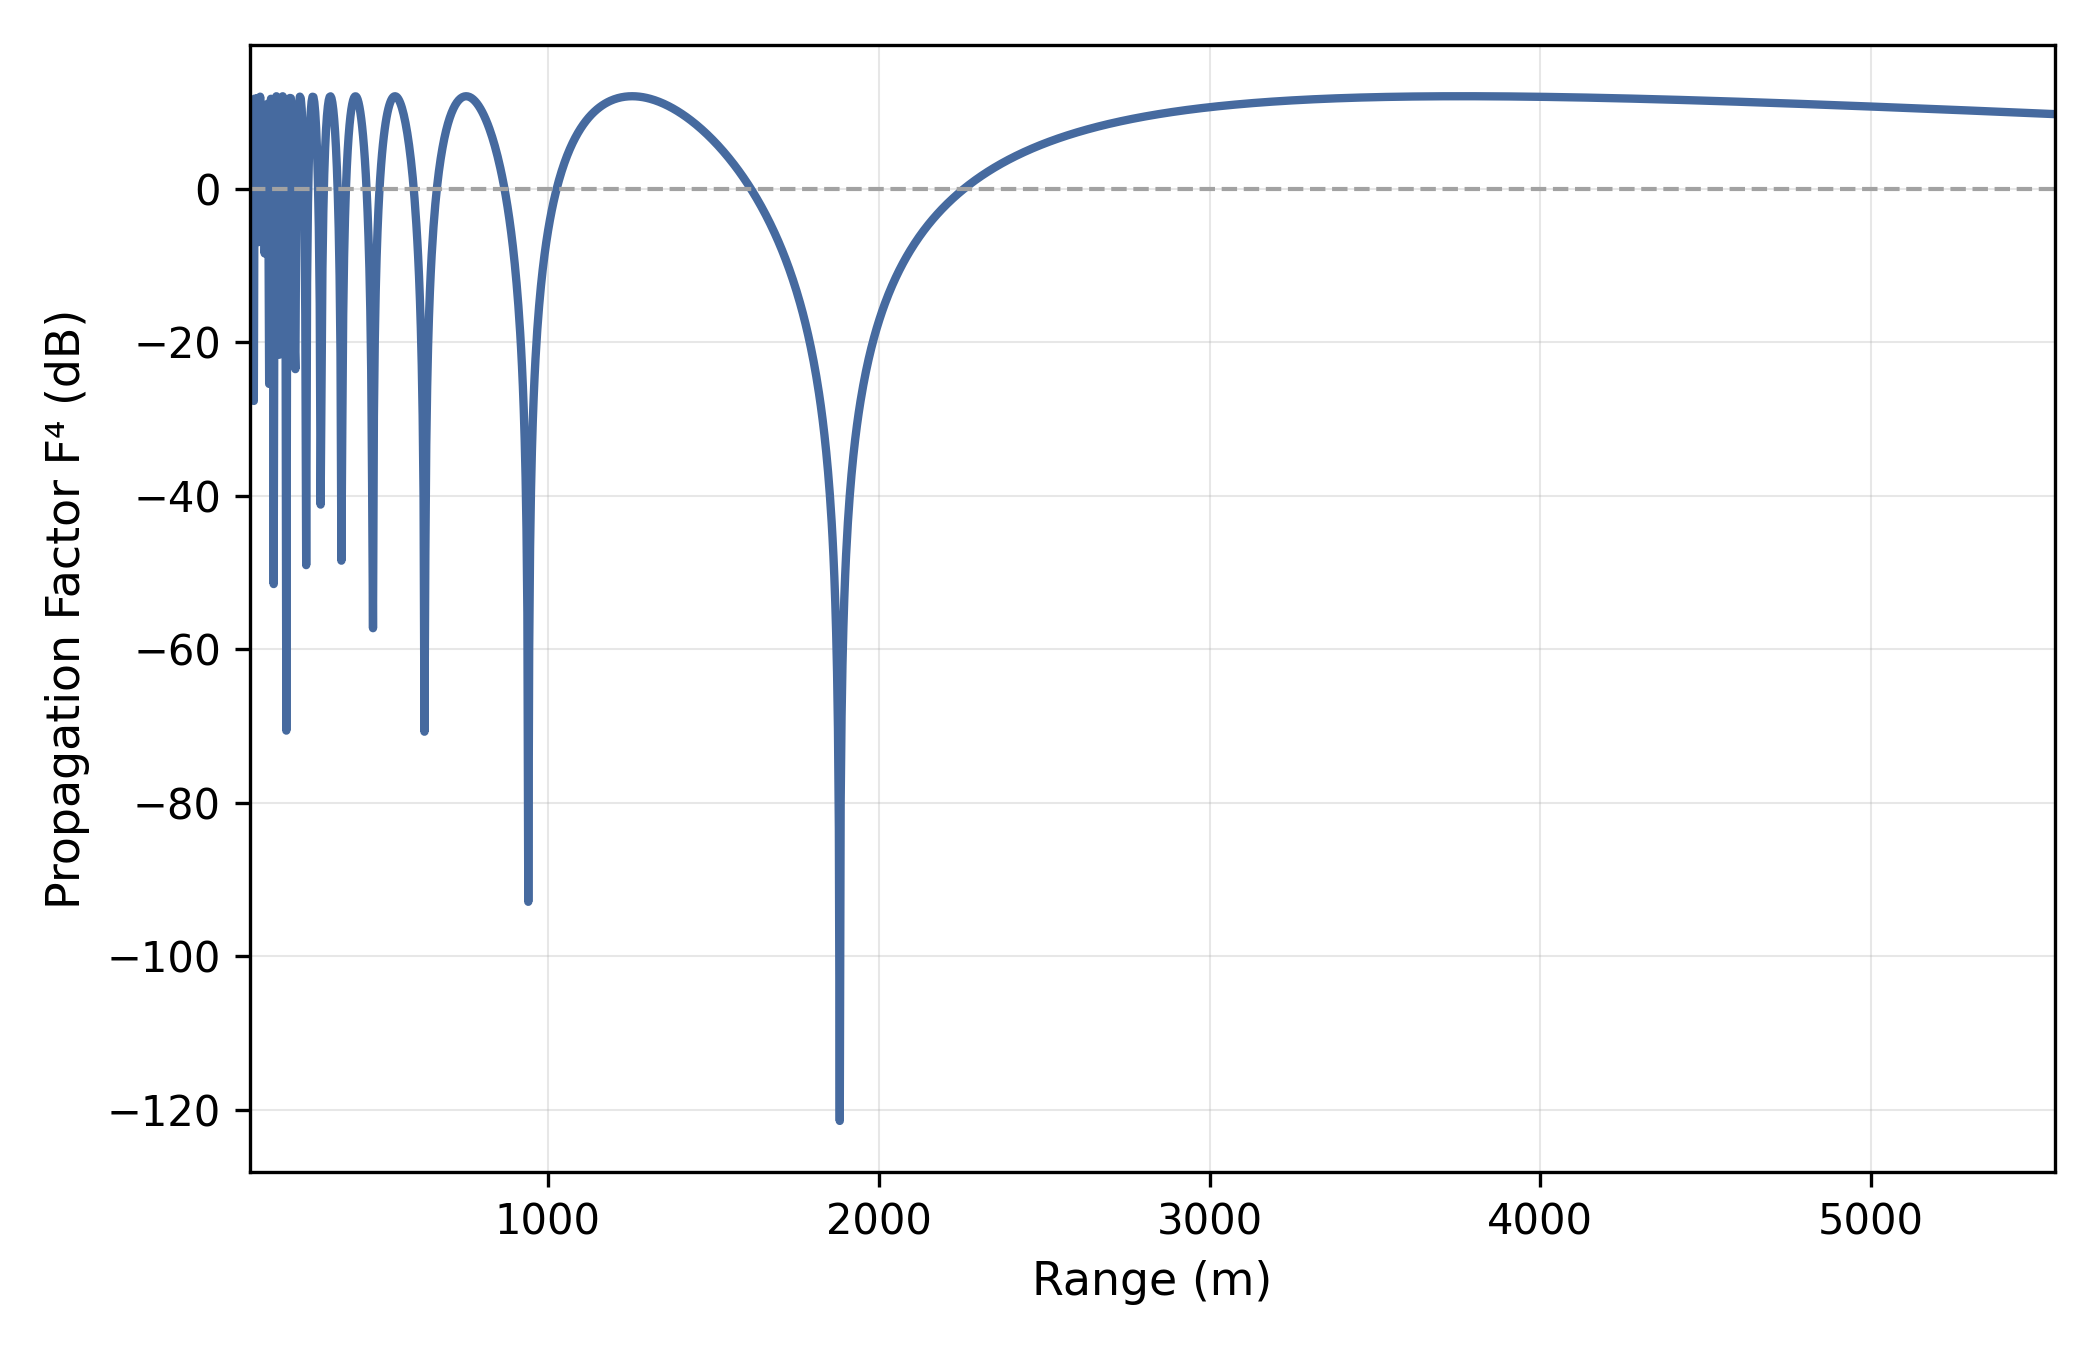
\includegraphics[width=0.9\columnwidth]{multipath_f4.png}
\caption{Two-way multipath propagation factor $F^4$ vs.\ range for $h_{\mathrm{ant}} = 10$~m and $h_{\mathrm{tgt}} = 3$~m over seawater at 9.41~GHz.}
\label{fig:multipath_factor}
\end{figure}

\subsection{Tier 3: Dataset Generation}
Table~\ref{tab:dataset_summary} summarizes a representative dataset generated using the Tier~3 compositor.

\begin{table}[htb]
\centering
\caption{Tier~3 dataset generation summary.}
\label{tab:dataset_summary}
\begin{tabular}{@{}lr@{}}
\toprule
\textbf{Property} & \textbf{Value} \\
\midrule
Background frames available & 164 \\
Extracted object signatures & 1{,}847 \\
Generated training sequence & 1{,}000 frames \\
Generated evaluation sequence & 500 frames \\
Objects per frame & 5--20 \\
Object classes & vessel, buoy \\
Label formats & Polar + Cartesian YOLO \\
Output resolution & $720 \times 868$ (polar) \\
\bottomrule
\end{tabular}
\end{table}

\subsection{Cross-Tier Comparison}
Figure~\ref{fig:cross_tier} provides a visual comparison of PPI outputs from all three tiers for qualitatively similar maritime scenes. Tier~1 shows the most detailed scattering phenomenology; Tier~2 captures the statistical clutter and target characteristics with less spatial detail; Tier~3 produces the most visually realistic output by leveraging real recorded data.

\begin{figure}[htb]
\centering
\begin{subcaptionblock}{0.32\columnwidth}
    \centering
    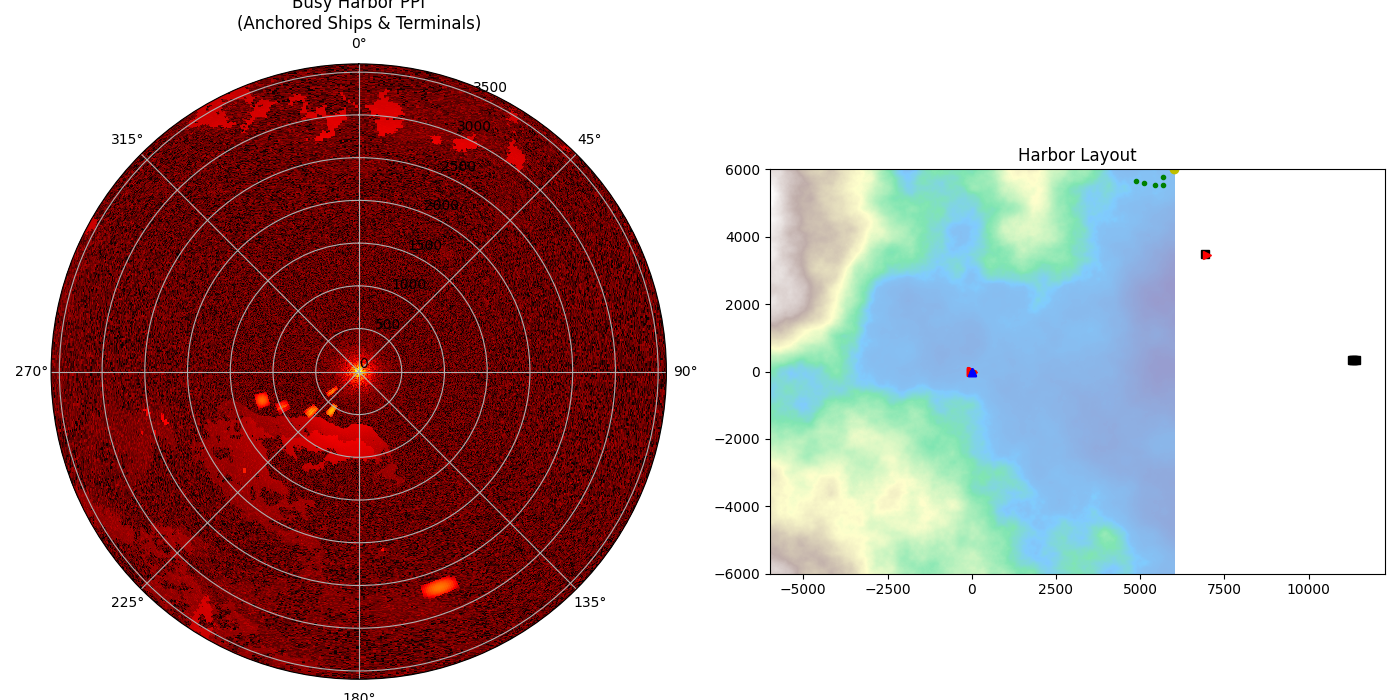
\includegraphics[width=\linewidth]{harbor_demo.png}
    \caption{Tier 1}
\end{subcaptionblock}
\hfill
\begin{subcaptionblock}{0.32\columnwidth}
    \centering
    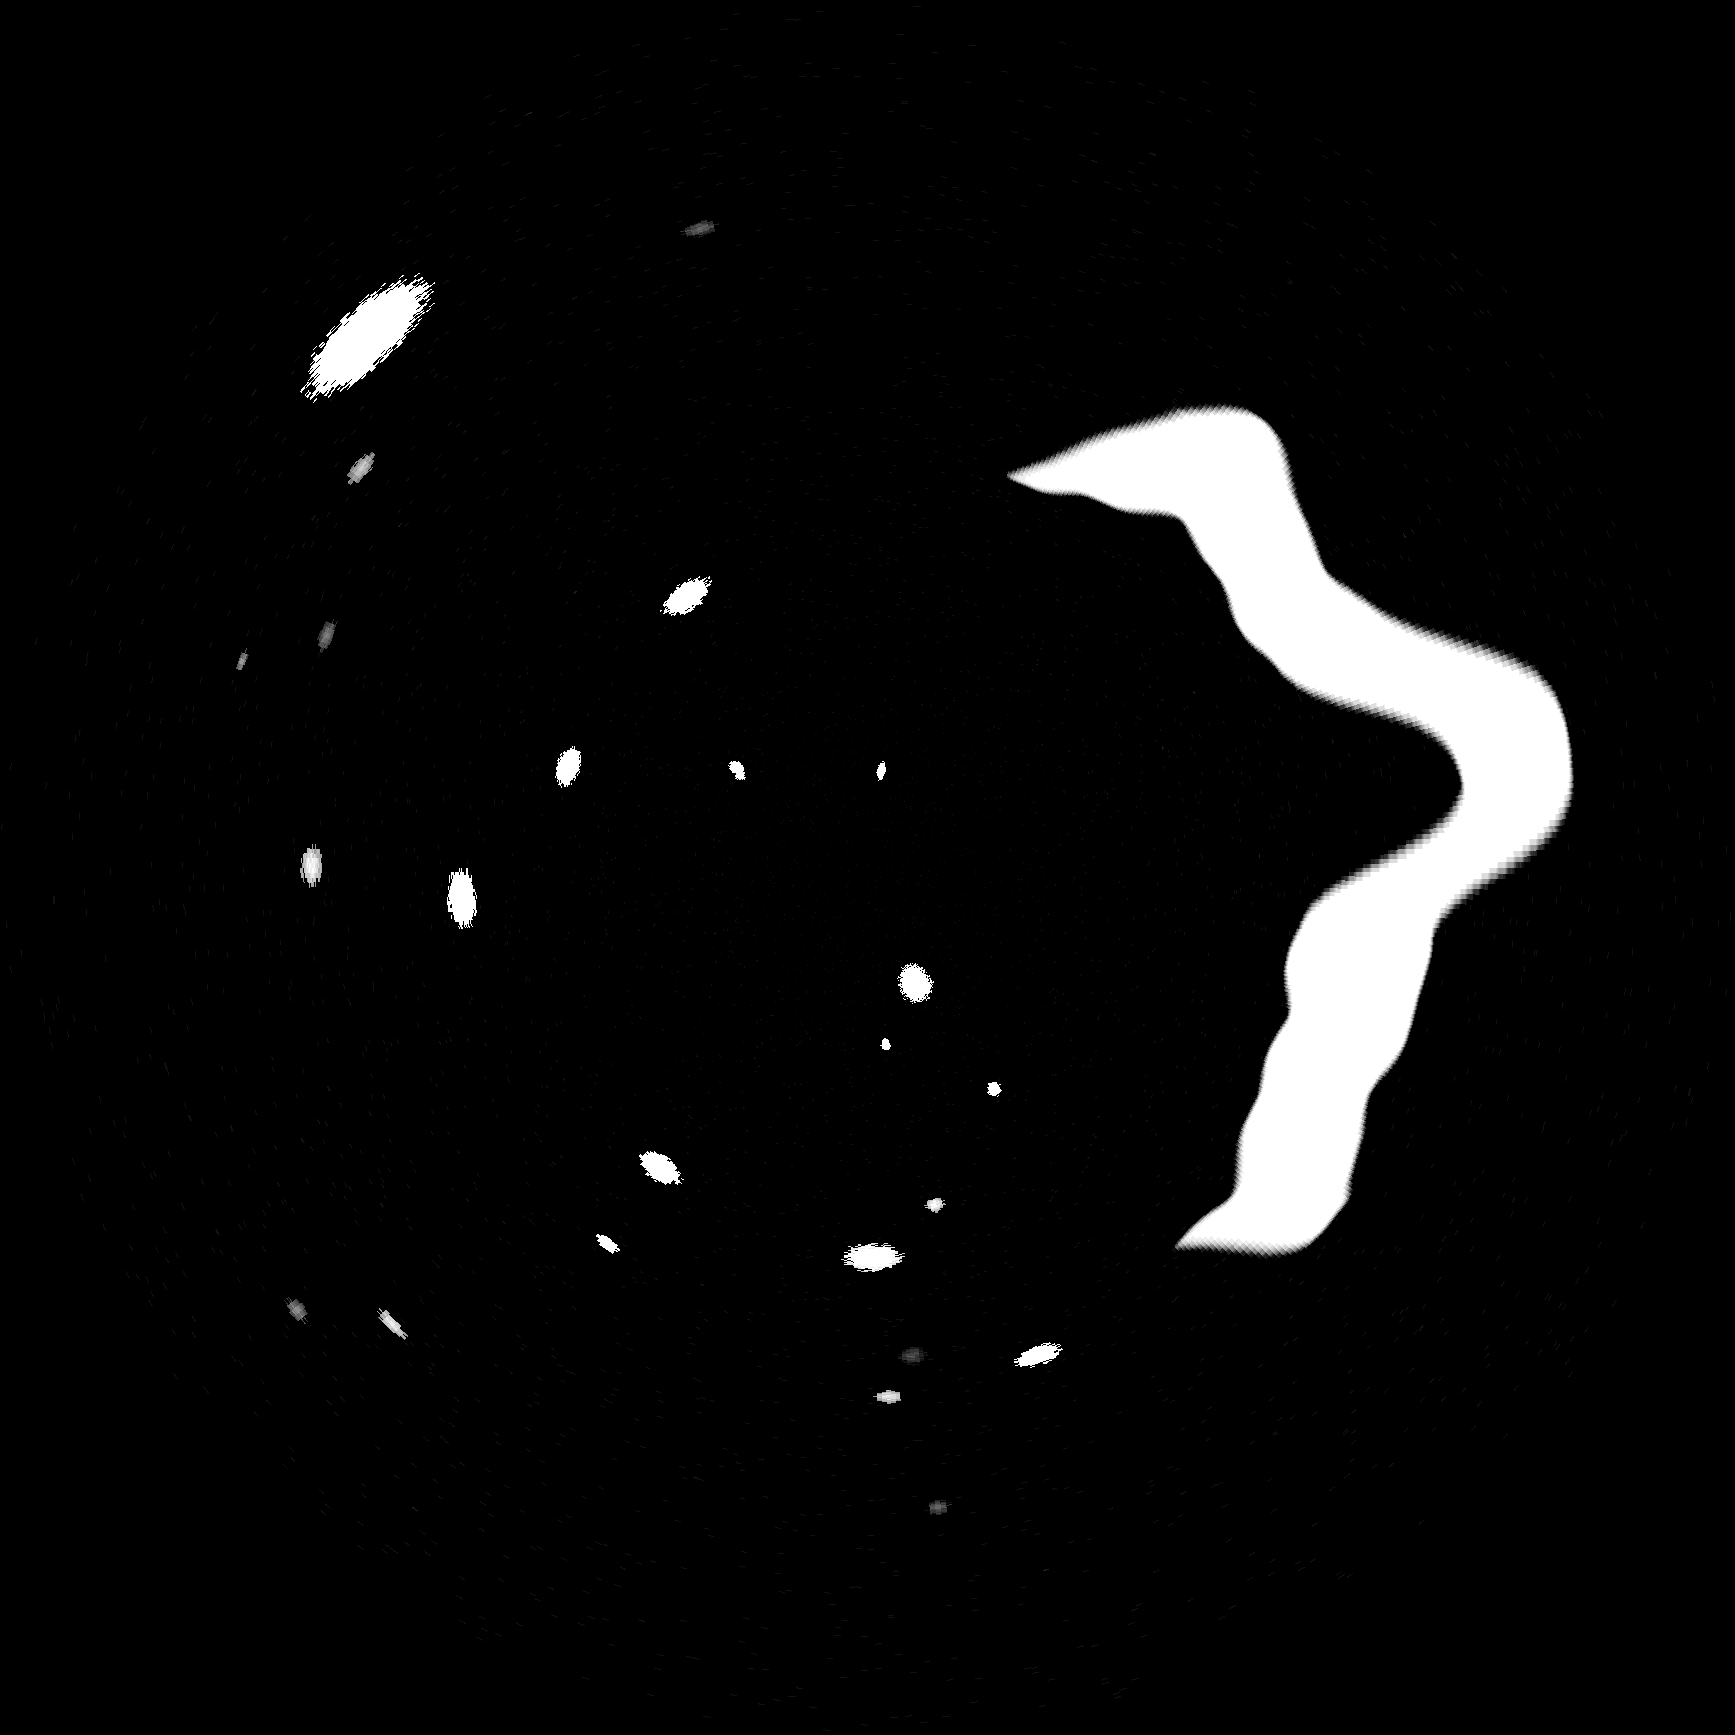
\includegraphics[width=\linewidth]{land_and_targets.png}
    \caption{Tier 2}
\end{subcaptionblock}
\hfill
\begin{subcaptionblock}{0.32\columnwidth}
    \centering
    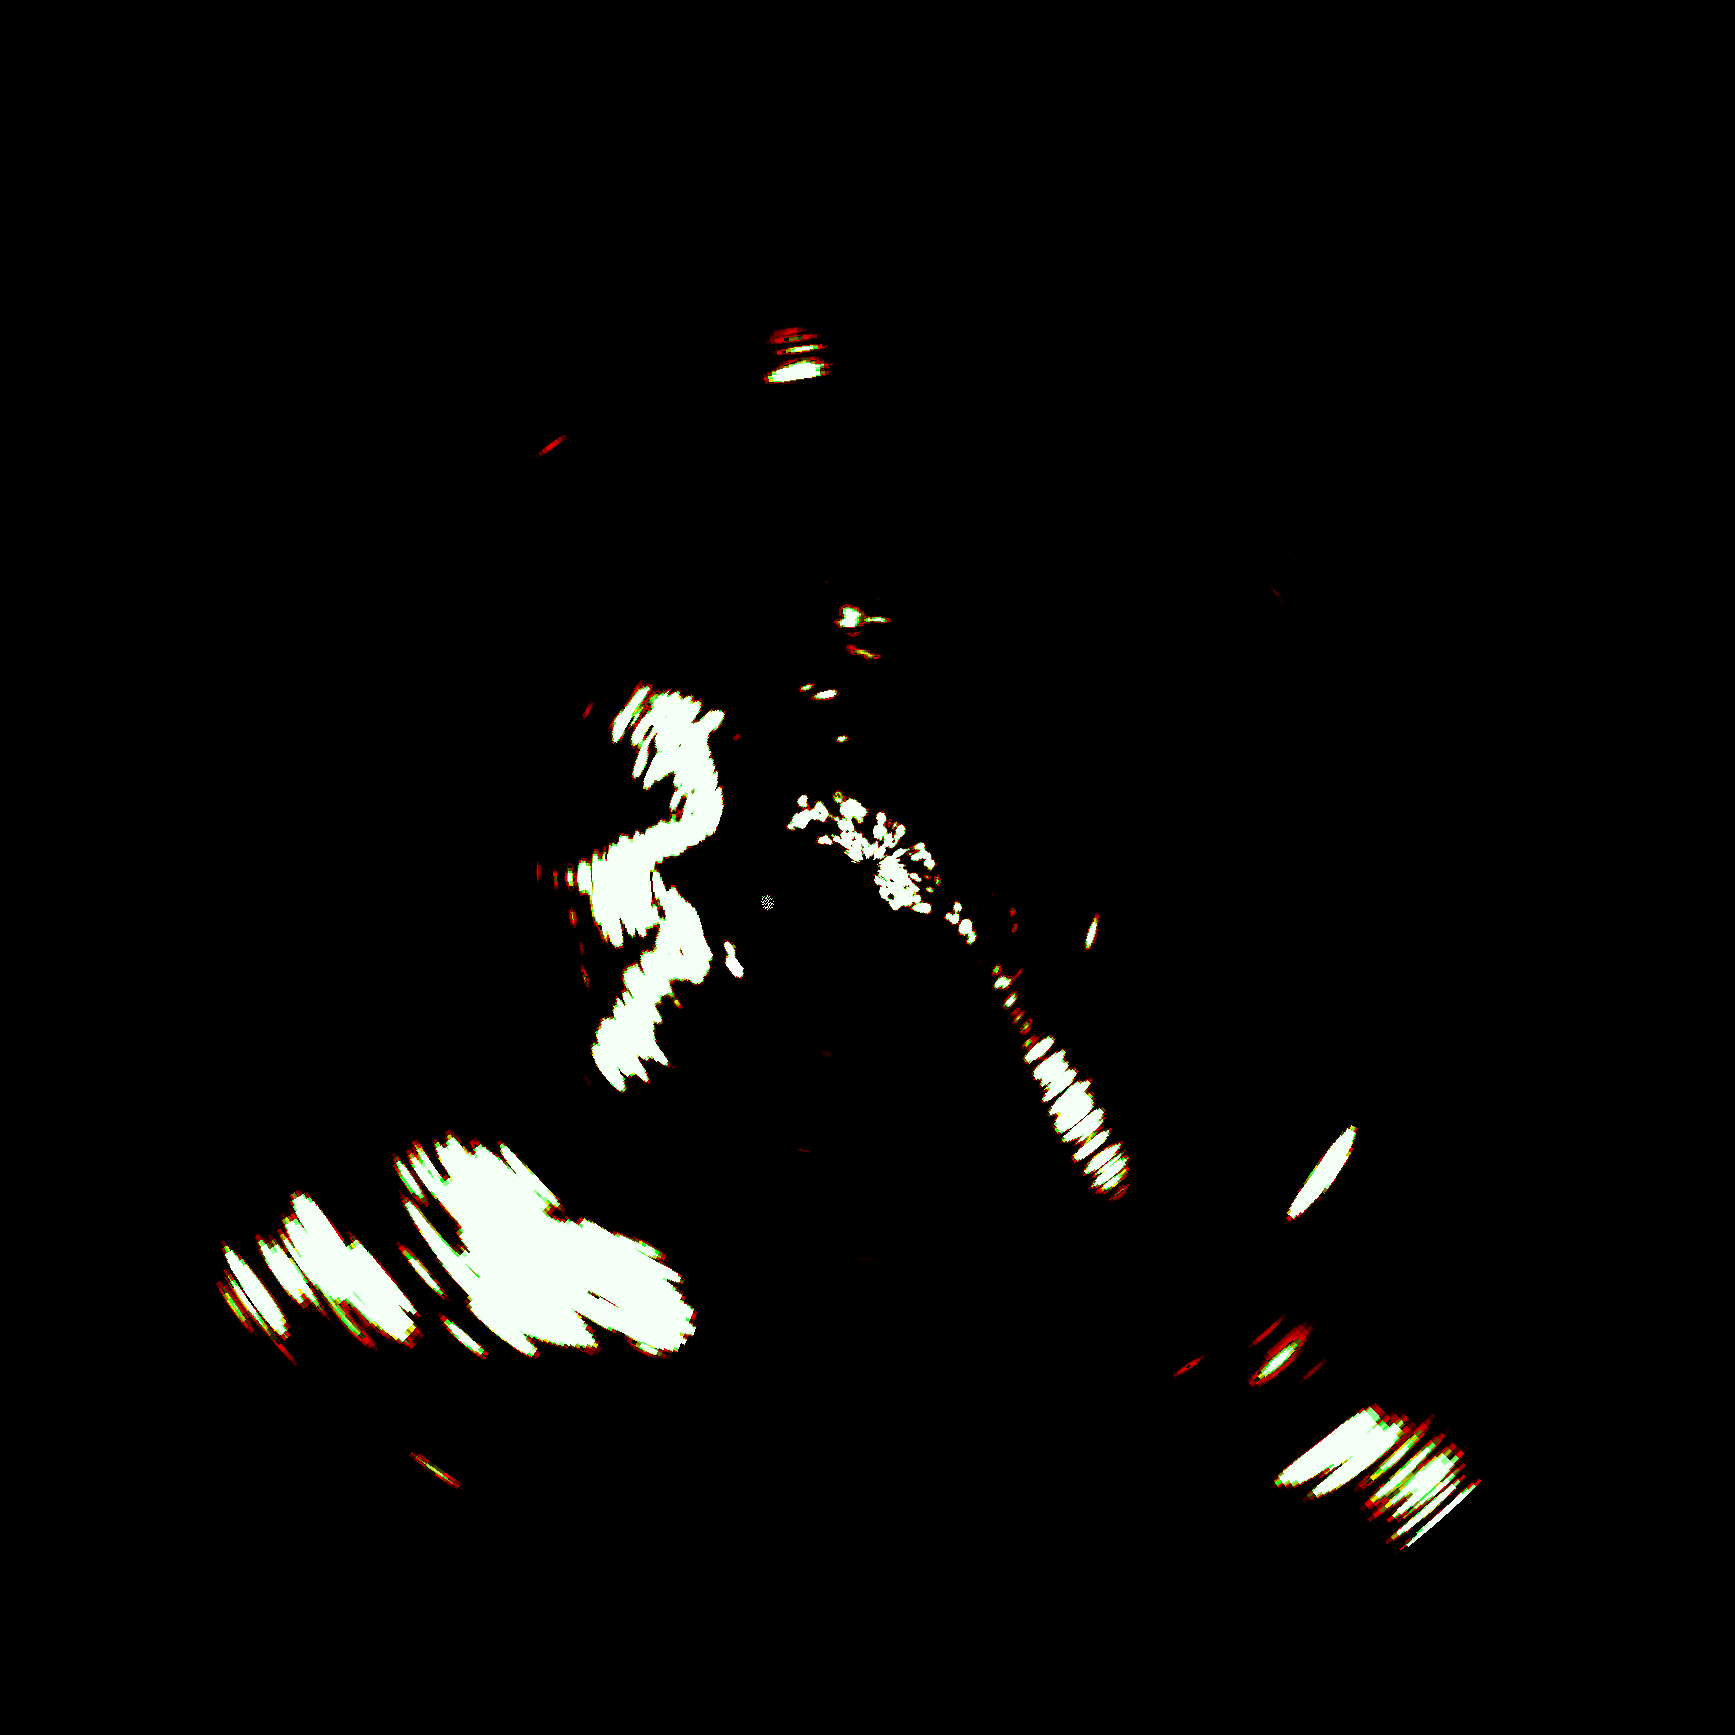
\includegraphics[width=\linewidth]{grayscale_frame.png}
    \caption{Tier 3}
\end{subcaptionblock}
\caption{Cross-tier visual comparison of PPI outputs. (a)~Tier~1 harbor scene with ray-traced EM scattering. (b)~Tier~2 analytical scene with K-distribution clutter and Swerling targets. (c)~Tier~3 composited scene from real recorded data.}
\label{fig:cross_tier}
\end{figure}

% ============================================================================
%  SECTION 9: DISCUSSION
% ============================================================================
\section{Discussion: The Model-Reality Gap}\label{sec:discussion}

Each tier of the framework makes simplifying assumptions that introduce a gap between simulated and real radar data. An honest assessment of these limitations is essential for appropriate use of the generated data.

\textbf{Tier~1} provides the most physically grounded simulation, but its computational cost (minutes per frame) limits the volume of training data that can be generated. Additionally, the PO approximation breaks down at very low grazing angles ($\psi < 2^\circ$) where shadowing and diffraction from the sea surface become dominant, and the SBR bounce model does not capture diffuse scattering from rough surfaces. The current implementation uses CPU-vectorized ray tracing rather than GPU acceleration, further limiting throughput.

\textbf{Tier~2} generates data rapidly, but the statistical clutter models assume spatial stationarity within a given range ring and do not capture the spatial coherence of real sea clutter patterns. Range-dependent shadowing by wave crests, which produces the characteristic ``speckle structure'' in real high-sea-state returns, is absent. The Swerling target models assume independent draws from a prescribed distribution without modeling aspect-angle dependence or the detailed scattering mechanisms that produce RCS fluctuations.

\textbf{Tier~3} produces the most visually realistic output because it operates on real recorded data, but it is limited by the finite size of the extracted object library (1{,}847 signatures from current recordings). Objects are composited without range- or aspect-dependent intensity correction, meaning an object signature extracted at one range is pasted at another range without the $1/R^4$ correction that physics would dictate. Additionally, the echo-trail model is a simple exponential decay rather than a calibrated persistence model matching the Furuno display hardware.

The multi-fidelity architecture mitigates these individual limitations by enabling cross-tier validation: Tier~1 can validate that Tier~2's statistical assumptions produce reasonable aggregate behavior, and Tier~3 provides a reality check against actual sensor data. A detector trained on Tier~2 data can be evaluated on Tier~3 composites to estimate the domain gap before deployment on real recordings.

% ============================================================================
%  SECTION 10: CONCLUSION
% ============================================================================
\section{Conclusion and Future Work}\label{sec:conclusion}

This paper presented a multi-fidelity simulation framework for X-band marine radar comprising three computational tiers that span from first-principles electromagnetic ray tracing to data-driven compositing. The framework addresses a critical gap in the development of radar-based maritime perception systems: the scarcity of diverse, labeled training data.

The three tiers serve complementary roles in the algorithm development cycle. Tier~1's SBR-PO-PTD ray tracing provides physically rigorous validation data at modest throughput. Tier~2's analytical K-distribution clutter and Swerling target models generate statistically representative data at high volume. Tier~3's compositor produces the most visually realistic data by blending real object signatures into recorded radar backgrounds. All three tiers share a common sensor model, output format, and configuration system, enabling seamless cross-tier workflows.

Validation results demonstrate that Tier~1 reproduces analytical corner-reflector cross sections and generates visually plausible PPI imagery, that Tier~2's clutter statistics match the theoretical K-distribution, and that Tier~3's compositor produces labeled datasets suitable for training YOLO-family detectors.

Future work will pursue several directions:
\begin{itemize}
    \item \textbf{GPU ray tracing}: Porting the Tier~1 SBR engine to GPU (e.g., NVIDIA OptiX) to reduce per-frame time from minutes to seconds, enabling physics-based data at Tier~2 throughput levels.
    \item \textbf{NeRF-based scenes}: Replacing triangulated mesh representations with neural radiance fields for more compact and differentiable scene descriptions.
    \item \textbf{Weather coupling}: Integrating atmospheric propagation models (ducting, rain attenuation) across all tiers for consistent environmental fidelity.
    \item \textbf{Library expansion}: Growing the Tier~3 object library through active deployment of the Furuno system in diverse maritime environments.
    \item \textbf{Formal sim-to-real transfer studies}: Quantifying detection and tracking performance degradation when algorithms trained on each tier's synthetic data are deployed on real recordings.
    \item \textbf{Tracker integration}: Coupling the framework with the companion ST-DBSCAN-based maritime object tracker to enable end-to-end perception pipeline evaluation.
\end{itemize}

\section*{Acknowledgments}

\bibliography{references}

\end{document}
